\documentclass[11pt]{report} % For LaTeX2e


%%%%%%%%%%%%%%%%%%%%%%%%%%%%%%%%%%%%%%%%%%%%%%%%%%%%%%%%%%%%%%%%
%% Recommended (but not required) packages
%%%%%%%%%%%%%%%%%%%%%%%%%%%%%%%%%%%%%%%%%%%%%%%%%%%%%%%%%%%%%%%%
\usepackage{amssymb}            % Defines common symbols like \mathbb R
\usepackage{mathtools}          % Extends amsmath, providing common math tools
\usepackage{mathrsfs}           % Enables \mathscr, which can work in cases that \mathcal does not
%\mathtoolsset{showonlyrefs}     % Only number equations that are referenced (optional)
\usepackage{graphicx}           % For including images
\usepackage{subcaption}         % Allows for the use of subfigures and subcaptions
\usepackage[space]{grffile}     % For spaces in image names
\usepackage{url}                % For displaying urls
\usepackage{amsmath}
\usepackage[urlcolor=blue]{hyperref}
\usepackage[parfill]{parskip}   % no indentation between paragraphs
\usepackage{xcolor}             % for the colors
\usepackage{makecell}           % for multirow in tables

\usepackage{algorithm}
\usepackage{algpseudocode}



\DeclareMathOperator{\E}{\mathbb{E}} %for expectation symbol

%%%%%%%%%%%%%%%%%%%%%%%%%%%%%%%%%%%%%%%%%%%%%%%%%%%%%%%%%%%%%%%%
%% Bibliography
%%%%%%%%%%%%%%%%%%%%%%%%%%%%%%%%%%%%%%%%%%%%%%%%%%%%%%%%%%%%%%%%
\usepackage{natbib}
\bibliographystyle{abbrvnat}
\setcitestyle{authoryear,open={(},close={)}} %Citation-related commands




%%%%%%%%%%%%%%%%%%%%%%%%%%%%%%%%%%%%%%%%%%%%%%%%%%%%%%%%%%%%%%%%
%% Begin document, create title and abstract
%%%%%%%%%%%%%%%%%%%%%%%%%%%%%%%%%%%%%%%%%%%%%%%%%%%%%%%%%%%%%%%%
\begin{document}

\begin{titlepage}
\begin{figure}[!htb]
    \centering
    
\includegraphics[keepaspectratio=true,scale=0.5]{images/Frontespizio/cherubinFrontespizio-eps-converted-to}
\end{figure}

\begin{center}
    \LARGE{UNIVERSITY OF PISA}
    \vspace{5mm}
    \\ \large{Department of Computer Science}
    \vspace{5mm}
    \\ \LARGE{Master's Degree in Computer Science}
    \\ \LARGE{Curriculum: Artificial Intelligence}
\end{center}

%adaptively combining
%abstract piccolissimo rl, dinamicamente adattare, lifelong learning, agents

\vspace{7mm}
\begin{center}
    {\LARGE{\bf Adaptively combining skill embeddings for Reinforcement Learning agents' state representation\\ \vspace{5mm}
    }}
    
    % Se il titolo è abbastanza corto da stare su una riga, si può usare
    
    % {\LARGE{\bf Un fantastico titolo per la mia tesi!}}
\end{center}
\vspace{15mm}

\begin{minipage}[t]{0.47\textwidth}
	{\large{Relatore:}{\normalsize\vspace{3mm}
	\bf\\ \large{Prof: Nome Cognome} \normalsize\vspace{3mm}\bf \\ \large{Prof: Nome Cognome}}}
\end{minipage}
\hfill
\begin{minipage}[t]{0.47\textwidth}\raggedleft
	{\large{Candidato:}{\normalsize\vspace{3mm} \bf\\ \large{Nome Cognome}}}
\end{minipage}

\vspace{10mm}
\hrulefill
\\\centering{\large{ACADEMIC YEAR 2023/2024}}

\end{titlepage}
\begin{abstract}

TODO - EXTEND

%Reinforcement Learning consists on maximizing the cumulative reward obtained by an agent interacting with the environment.
%Standard approaches learn an end-to-end mapping from observations to action spaces which define the agent's behavior.
% On the other hand, Foundational Models learns different representations of the world which can be used by agents to accelerate the learning process.
% In this thesis we studied how to combine these representations to create an enhanced state representation.
% Specifically we propose a technique called Weight Sharing Attention (WSA) which combines embeddings of different Foundational Models, and we compare different combination modes.
%We tested our approach on different Atari games, and we analyzed the issue of out of distribution data and how to mitigate it.
%We showed that, without fine-tuning of hyperparameters, WSA obtains comparable performance with state-of-the-art methods.
%This method is effective and could allow life-long learning agents to adapt to different scenarios over time.

%via agent's interaction with a specific environment. Usually, the go-to approach to tackle this problem is to learn from scratch an end-to-end mapping between the observation and action spaces to define agents' behaviors.
%On the other hand, Foundational Models (FMs) can share insightful representations of the world ready to be leveraged by agents. Different FMs learn disparate latent embeddings, also coming from different modalities. How to effectively combine these representations is still an open and understudied question.
%In this work, we propose Weight Sharing Attention (WSA) to combine embeddings of different FMs to shape an enriched state representation. We compare several combination modes showing that, without fine-tuning of hyperparameters, WSA obtains comparable performance with state-of-the-art methods on different Atari games. Furthermore, we demonstrate and analyse one of the principal challenges and limitations of this approach: the issue of out of distribution data.



%In this work, we present a technique for deep reinforcement learning that, through the use of different state representations, is able to combine different features in order to create an enhanced feature rapresentation.
%Instead of directly learning a policy from raw input, the agent uses pre-trained foundational models which are capable of extracting features of various forms.

\end{abstract}


\tableofcontents

% Rimuovere se non si vuole la tabella delle figure
%\listoffigures

%! Author = giaco
%! Date = 16/05/2024

\chapter{Introduction}
\label{sec:introduction}
Reinforcement Learning \citep{sutton1998introduction} is one of the paradigms of Machine Learning (ML). It consists of having an agent learn the optimal behavior in an environment that can change over time to maximize the cumulative reward that it obtains as a consequence of its actions.
In particular, RL mimics how we, as humans, learn.
It formulates the learning process as a sequence of interactions with the environment and uses a trial-and-error approach to process data.
Agents learn to solve a specific task based on their experiences with the world, they learn from the feedback of each action and discover the best way to achieve their goal.

Over the past decades, RL algorithms have increasingly improved, achieving amazing results in many tasks and being adopted in new fields.
For example, RL can be applied in many real-world scenarios, some of them are applications like recommendation systems where RL agents can customize suggestions to individual users based on their interactions, or for financial predictions where RL algorithms can optimize long-term returns by considering transaction costs and adapting to market shifts. 
Finally, it can be used in industry automation to teach robots to act more efficiently than humans or for self-driving cars and many other applications.

%To name a few important works that are noteworthy throughout the history of RL, \citet{watkins1992q} introduced \textbf{Q-Learning}, which is an RL algorithm to learn the value of an action in a particular state and has become one of the most well-known and widely used RL algorithms.
%\citep{sutton1999policy} instead, introduced policy gradient methods that are very useful, especially in scenarios involving continuous action spaces.

Some recent achievements in RL that are related to the topics that will be developed in this thesis are
the works of \citet{mnih2013playing, mnih2015human}, which started to explore the use of deep neural networks in games, specifically using the Arcade Learning Environment (ALE) \citep{bellemare2013atari}.
As a result of these works, although based on problems that may seem as basic as those in video games, new development perspectives have been created and an increasing interest has turned toward Deep Reinforcement Learning (DRL).
In fact, DRL has produced substantial advancements in various research fields and applications, such as games as already mentioned, beating all Atari games at super-human performance with a single algorithm \citep{agent57} or defeating pro players in games like GO, StarCraft II and DOTA \citep{alphago, starcraft, dota}, but also in robotics \citep{rlrob, bousmalis2023robocat} and lastly toward general agents for 3D environments including different data modalities \citep{sima2024}.

Discussing some of the problems highlighted in this thesis concerning the current algorithms in the literature, in a typical RL setting, agents receive as input the raw representation of the state, without any additional information on the elements that characterize it.
Learning, which comprises creating a map from input to action space, i.e. creating a policy,  for an RL agent consists of training a model from scratch every time to solve one specific task and, therefore, requires a lot of interaction with the environment to perform well, much more than the number of actions a human would need.
End-to-end solutions for the learning process implicitly hide a significant effort related to understanding how to process the input representations in the best possible way.
While one of the promises of deep learning algorithms is to automatically construct well-tuned representations, the same might not emerge from the training of deep RL agents. 
This is because agents learn how to solve the task while indirectly learning how to process and extract useful information from the input features. 
While this approach has been the solution for several works, it adds a layer of complexity to RL algorithms eventually requiring significant computational resources.

Several works analyze the differences between the learning process of humans and RL agents, highlighting how prior knowledge can influence the learning curve \citep{lake2017building, dubey2018investigating}.
Agents, in the same way as humans, can define the learning pattern by incrementally improving their abilities.
Learning for humans, however, consists of acquiring new skills and incrementally improving those already known, leveraging prior knowledge, and adapting strategies based on experience.
In new environments with few interactions, humans can make use of their prior abilities to accomplish basic tasks like distinguishing new elements or reading guidelines.
Humans can understand the effects of their actions and this allows them to focus mostly on learning a good policy, rather than also learning how to interpret the environment. 
The idea behind this thesis is, therefore, to provide RL agents with abilities, just like humans, and aims to study a way to encode skills in such a way to incorporate prior knowledge into an RL agent.
In this way, we can focus on how RL agents can exploit prior knowledge provided their abilities and focus the learning process on the actual policy.

In the development of this thesis, we will then try to answer two questions:
\begin{itemize}
    \item How can we represent skills for an RL agent?
    \item Once skills are defined, how can we encode them and combine information coming from different skills or choose which one to use?
\end{itemize}

To answer the first question, Foundation Models (FMs) present themselves as good candidates.
FMs refer to large-scale, pre-trained models that serve as a base for various downstream tasks.
Examples of FMs, can be \citet{brown2020language, devlin2018bert, he2016deep}
They are trained on extensive datasets in a self-supervised fashion, enabling them to learn rich and generalizable representations that can be fine-tuned or adapted for specific applications. 
These representations can be leveraged in RL to accelerate the learning process and improve performance on complex tasks. Using FMs' knowledge, RL agents can achieve higher efficiency and effectiveness, even in environments with sparse rewards or limited data. 
As for the latter question, instead, this thesis aims to study how different FM embeddings can be combined in several ways to compute a rich and informative representation of the environment. 


In short, we will use relatively small models, but all the work can be scaled without additional effort, and we propose, among the other ways of combining information, Weight Sharing Attention (WSA) as a combination module to incorporate different encodings coming from several FMs.
We executed experiments across three different Atari games that are \textit{Pong}, \textit{MsPacman}, and \textit{Breakout} and we studied the behavior of 7 different combination modules.
WSA achieves comparable performance with end-to-end solutions, while also adding scalability and explainability to RL agents.
We show that without any fine-tuning of hyperparameters, our methodology can achieve competitive results with established RL end-to-end solutions. Moreover, we prove and address the problem of out-of-distribution data, which presents itself as one of the main challenges for these approaches. 


The thesis is organized in this way: Ch.\ref{sec:background} will introduce and explain all the techniques that are adopted in this work. Ch. \ref{ch:related_work} provides information about related works and current state-of-the-art. Ch. \ref{sec:method} shows information about our approach. Ch. \ref{ch:experiments} provides the experiments that we conducted to test our method. Ch. \ref{sec:results} shows the results and finally Ch. \ref{sec:conclusions} provides the conclusions of the work and discusses possible future extensions.


%! Author = giaco
%! Date = 16/05/2024

\chapter{Background}
\label{sec:background}
In this chapter, we provide a brief overview of the main concepts that are necessary to understand the work presented in this thesis.
First of all, we start by introducing the concept of Machine Learning (ML) and Deep Learning (DL) in~\ref{sec:machine_learning}.
Then, in~\ref{sec:rl} we will talk in depth about one specific kind of learning, i.e.\ Reinforcement Learning, which is instead the main focus of this work, and we will talk also about Deep Reinforcement Learning (DRL).

\section{Machine Learning}
\label{sec:machine_learning}
%inserire immagine AI-ML-DL
% prendi immagini da qui https://www.geeksforgeeks.org/types-of-machine-learning/

Machine Learning, Fig. \ref{fig:ml_hierarchy}, is the branch of Artificial Intelligence that focuses on developing models and algorithms that let computers learn from data and improve from previous experience without being explicitly programmed for every task.
In simple words, ML teaches the systems to think and understand like humans by learning from the data.
ML finds application in many fields, including natural language processing, computer vision, speech recognition, email filtering, medicine, and many more

There are several types of ML family of algorithms, each with its own characteristics and applications.
Some of the main types are Supervised Learning, Unsupervised Learning, Self-Supervised Learning, and finally Reinforcement Learning, Fig.\ref{fig:ml_types}
A subset of ML is Deep Learning, which focuses on training neural networks with many layers.

We will talk about the different kinds of learning algorithms and DL in the following subsection, while since RL is the focus of this work we will dedicate a proper section.





\begin{figure}[ht]
    \begin{subfigure}[b]{0.45\textwidth}
        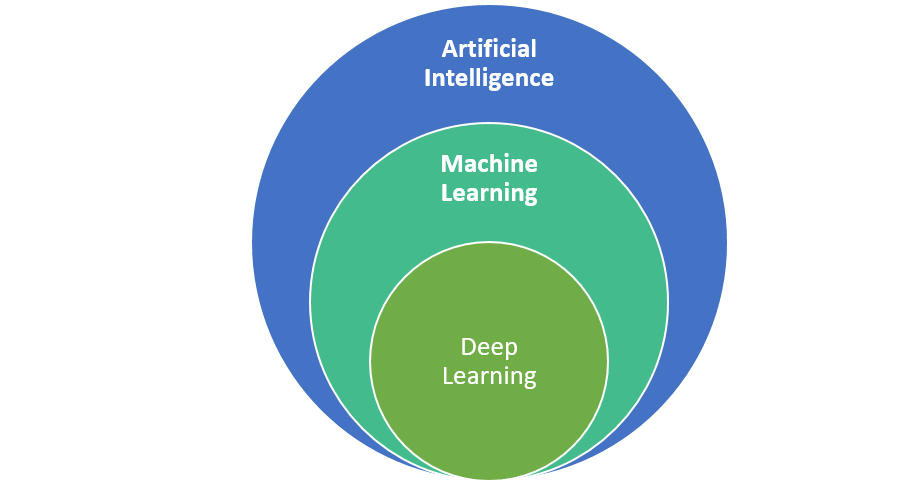
\includegraphics[width=\textwidth]{images/background/ai_ml_dl}
        \caption{\texttt{Artificial Intelligence hierarchy.}}
        \label{fig:ml_hierarchy}
    \end{subfigure}
    \hfill
    \begin{subfigure}[b]{0.45\textwidth}
        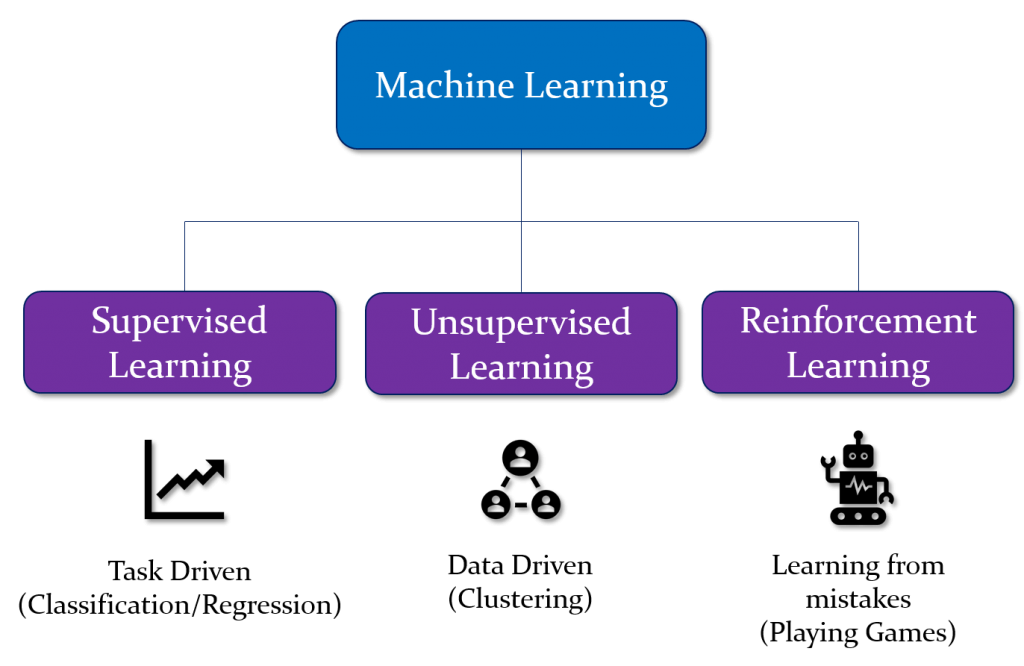
\includegraphics[width=\textwidth]{images/background/ML_Types}
        \caption{\texttt{Some Families of ML algorithms.}}
        \label{fig:ml_types}
    \end{subfigure}
    \hfill
    
\end{figure}








\subsubsection{Supervised Learning}
\label{subsubsec:supervised_ml}
%insert citation of examples of supervised learning?
Supervised Learning is a type of ML where the model is trained on a labeled dataset.
In this context, \textit{labeled} means that each training example is paired with an output label.
The goal of supervised learning is to learn a mapping from inputs to outputs that can be used to predict the output for new, unseen inputs.


There are two main categories of supervised learning that are:
\begin{itemize}
    \item Classification - The goal is to predict a discrete label.
    For example, classifying emails as spam or not spam, or recognizing handwritten digits.
    Classification algorithms learn to map the input features to one of the predefined classes.

    \item Regression - The goal is to predict a continuous value.
    For example, predicting the price of a house given its features, or the temperature for a given day.
    Regression algorithms learn to map the input features to a continuous numerical value.

\end{itemize}

%advantages and disadvantages
Supervised Learning models can have high accuracy as they are trained on labeled data. Also, they can be used as pre-trained models, which saves time and resources when developing new models from scratch.
They have some limitations though, in fact, sometimes they need a huge amount of data to perform well and they may struggle with unseen or unexpected patterns that are not present in the training data. Finally, they can be time-consuming when in the presence of a huge amount of data in the training set.

\subsubsection{Unsupervised Learning}
\label{subsubsec:unsupervised_ml}
Unsupervised learning is a type of ML technique in which an algorithm discovers patterns and relationships using unlabeled data.
Unlike supervised learning, unsupervised learning doesn’t involve providing the algorithm with labeled target outputs.
The primary goal of Unsupervised learning is often to discover hidden patterns, similarities, or clusters within the data, which can then be used for various purposes, such as data exploration, visualization, dimensionality reduction, and more.


The main categories of unsupervised learning are:
\begin{itemize}
    \item Clustering - This is the process of grouping data points into clusters based on their similarities.

    \item Association Rule learning - It is a method used for finding relationships between variables in a large database. A typical example of the Association Rule is the Market Basket Analysis which determines the set of items that occur together like people who buy a specific item also tend to purchase another item.

\end{itemize}


%advantages and disadvantages
Unsupervised Learning helps discover hidden patterns and relationships when labels for data are not available.
Without using labels though, it may be difficult to predict the quality of the model's output.





\subsubsection{Self-Supervised Machine Learning}
\label{sec:semisupervised_ml}
Self-supervised learning is a type of ML technique that falls in between supervised and unsupervised learning.
When in presence of a large amount of unlabeled data, self-supervised learning can be used to learn useful representations of the data.
In fact, it consists of pre-training a model using unlabelled data and generating data labels automatically. Then in the second phase, the algorithm uses the high-confidence data labels among those generated to train the model again in subsequent iterations, like the supervised learning method. The only difference is that the data labels used as ground truth in every iteration are changed.

Self-supervised learning is a powerful technique that can be used to learn useful representations of the data, and it can be used as a pre-training step for supervised learning tasks.
Self-supervised learning models were used in the development of this thesis as we will see in section INSERT.



\subsubsection{Deep Learning}
\label{sec:dl}
Deep Learning is a subfield of ML that, in the last years, has gained a lot of attention and has been successful in many fields.
It can be used in supervised, unsupervised, and self-supervised learning tasks, and it focuses on training neural networks with many layers, where each layer is responsible for extracting features from the input data at different levels of abstraction.

Specifically, a Neural Network (NN) is an Artificial Intelligence method that is inspired by the way the human brain works.
Every NN, consists of layers of interconnected nodes, which are called neurons.
A neuron is a computational unit that takes multiple inputs, multiplies them by weights, and sums them up, and applies an activation function to produce an output.
Activation functions are used to decide whether a neuron should be activated or not based on the weighted sum of the inputs.
They can be linear or non-linear functions, and they introduce non-linearity in the model, which allows the model to learn more complex patterns in the data rather than linear ones.
Examples of non-linear activation functions are the sigmoid, the ReLU, and the tanh function.

In specific, the computation of a neuron can be expressed as:

\begin{equation}
    y = f(\sum_{i=1}^{n} w_i x_i + b)\label{eq:neuron}
\end{equation}

Where $y$ is the output of the neuron, $f$ is the activation function, $w_i$ are the weights, $x_i$ are the inputs, and $b$ is the bias term.
Fig. \ref{fig:single_neuron} shows a picture of a single neuron.
It is possible to see a NN as a composition of multiple neurons, where the output of one neuron is the input of the next one.
We define Multilayer Perceptron (MLP) as a sequential model that is composed of multiple layers of neurons.
We have an input layer, which is responsible for receiving the input data, one or more hidden layers, that are responsible for processing the data in a way that encodes the information in a latent space, and finally an output layer, which is responsible for producing the output information.
In specific, we talk about feed-forward neural networks, when the information flows from the input layer to the output layer without any feedback connections, and we talk about fully-connected neural networks when each neuron in a layer is connected to every neuron in the next layer.
The mathematical representation of a feed-forward neural network is expressed in Eq. \ref{eq:nn}, while Fig. \ref{fig:nn} shows a picture of a feed-forward neural network.

\begin{equation}
    \hat{y} = f_n(f_{n-1}(\dots f_1(\sum_{i=1}^{n} w_i x_i + b_1) + b_{n-1}) + b_n)\label{eq:nn}
\end{equation}


The process of learning the weights relies on the backpropagation algorithm that consists of two main steps: forward pass and backward pass.

Suppose we are in a supervised learning setting, and we dispose to a dataset of input-output pairs $(x, y)$, where $x$ is the input data, and $y$ is the output data that we refer to as ground-truth.
In the forward pass, the input data is passed through the network, and the output \textit{\hat{y}} is computed.
Then, considering the output of the network, the error is computed using a loss function which is a distance metric and measures the difference between the predicted output and the true output.
A typical loss function is the Mean Squared Error (MSE) which is defined as:

\begin{equation}
    MSE = \frac{1}{n} \sum_{i=1}^{n} (y_i - \hat{y}_i)^2
\end{equation}

The backward pass consists of propagating the error back through the network, from output layer to the input one, and it is responsible for updating the weights to minimize the error between the predicted output and the ground-truth.
Weights are updated using the gradient descent algorithm, which is an optimization method that iteratively updates the weights in the direction of the steepest descent of the loss function.
In neural networks, backpropagation is implemented using the chain rule (of calculus) to compute the gradients of the loss function with respect to the weights.
Chain rule allowed to decompose the computation of the gradient of the loss function with respect to the weights into simpler computations, making the computation of the gradients more efficient and allowing the training of deep neural networks.
%insert figure



In the literature, multi-layered neural networks are referred to as Deep Neural Networks (DNNs), and the process of training them is called Deep Learning (DL).
One of the most successful architectures in deep learning is the Convolutional Neural Network (CNN), which is widely used in computer vision tasks.
CNNs are composed of:
\begin{itemize}
    \item convolutional layers, which applies a set of kernels to the input data to extract features.
    Each kernel extracts a different feature, and the output of a convolutional layer is a set of feature maps.
    \item activation functions, which introduce non-linearity in the model.
    \item pooling layers, which reduce the dimensionality of the data by reducing the size of feature maps.
    A typical example of pooling is the max-pooling, which takes the maximum value in a window of the feature map.
    \item fully connected layers, which takes as input the extracted features and makes the predictions.
\end{itemize}

Fig. \ref{fig:cnn} shows a picture of a CNN architecture.

%talk about feed forward nn vs cnn?

\section{Reinforcement Learning}
\label{sec:rl}

\subsection{Introduction}
% inserire reward hypothesis?
Reinforcement Learning is a paradigm of ML works in a way that mimics the trial-and-error learning process that humans use to achieve their goals.
The principle elements that comprise RL are the agent, the environment, and the reward signal.
The agent is the learner that interacts with the environment and RL focuses on training agents to make sequences of decisions in the environment to maximize a scalar reward signal.
In particular, in RL, there is no supervision.
The only feedback that the agent receives is the reward signal that indicates how well it is doing and should be informative enough to let the agent learn the optimal behavior.
Fig. \ref{fig:rl} shows a picture of the RL paradigm.

Environments can be fully observable when the agent has access to the complete state of the environment, or partially observable when the agent has access only to a partial observation of the environment.
Specifically, in the presence of fully observable environments, we formalize the RL problem as a Markov Decision Process (MDP), which is a tuple $(S, A, P, R, \gamma)$, where:
\begin{itemize}
    \item $S$ is the set of states that the agent can be in.
    \item $A$ is the set of actions that the agent can take.
    \item $P$ is the transition probability function, which defines the probability of transitioning from one state to another given an action.
    \item $R$ is the reward function, which defines the reward that the agent receives when transitioning from one state to another.
    \item $\gamma$ is the discount factor, which determines the importance of future rewards.
    If it is close to 0, the agent will consider only immediate rewards, while if it is close to 1, the agent will consider future rewards.
\end{itemize}

It is possible to define the return of an agent in an MDP as the sum of discounted reward from a specific timestep t.
In particular:
\begin{equation} \label{eq:return}
    G_t = R_{t+1} + \gamma R_{t+2} + \gamma^2 R_{t+3} + \dots = \sum_{k=0}^{\infty} \gamma^k R_{t+k+1}
\end{equation}

The principal components of an RL agent are three and in order are: the policy $\pi$, the value function $v$, and the model $m$.
The policy defines the behavior of the agent, and it is a mapping from states to actions.
Policy can be deterministic if it maps states to a single action, or stochastic if it maps states to a distribution over actions.
The policy can be represented as a table, a function, or a neural network and in the context of MDPs, the policy is defined as $\pi(a|s) = P(a|s)$, which is the probability of taking action $a$ in state $s$.


The value function estimates the expected return that the agent can achieve starting from a given state and following a given policy $\pi$.
It is used to evaluate how good a state is, and it is defined as:
\begin{equation} \label{eq:value_function}
    v_{\pi}(s) = \E_{\pi}[R_{t+1} + \gamma R_{t+2} + \gamma^2 R_{t+3} + \dots | S_t = s] = \E_{\pi}[G_t | S_t = s]
\end{equation}
This is also called the \textbf{state-value function}.
It exists an equivalent function that estimates the expected return that the agent can achieve starting from a given state, taking a specific action, and then following a given policy $\pi$.
This is called the \textbf{action-value function}, and it is defined in Eq. \ref{eq:action_value_function}.
Value functions too can be represented as tables, functions, or neural networks.

\begin{equation} \label{eq:action_value_function}
    q_{\pi}(s, a) = \E_{\pi}[R_{t+1} + \gamma R_{t+2} + \gamma^2 R_{t+3} + \dots | S_t = s, A_t = a] = \E_{\pi}[G_t | S_t = s, A_t = a]
\end{equation}


The model is used to predict what the environment will do next, so it is a representation of the environment and predicts the next state given current state and action, $P_{s, s'}^a = P(S_{t+1} = s' | S_t = s, A_t = a)$ and predicts the next reward given the current state and action, $R_s^a = \E[R_{t+1} | S_t = s, A_t = a]$.

The concept of learning in RL is based on the \textbf{Bellman Equations}, which form the basis for many RL algorithms and are divided into two main categories: the Bellman Expectation Equations and the Bellman Optimality Equations.
To estimates the goodness of a state, we can use the \textbf{Bellman Expectation Equations} for the state-value function and the action-value function, which provides a recursive relationship between the value of a state and the value of the next state.

Bellman Equation for state-value function is defined in Eq. \ref{eq:bellman_state_value} where the expected return is decomposed into the immediate reward and the discounted value of the next state, and then we marginalize over the actions to obtain the expected value of the state in terms of the action-value function.

\begin{equation} \label{eq:bellman_state_value}
    v_{\pi}(s) = \E_{\pi}[R_{t+1} + \gamma v_{\pi}(S_{t+1}) | S_t = s] = \sum_{a} \pi(a|s)q_{\pi}(s, a)
\end{equation}

Similarly, the Bellman Equation for the action-value function is defined in Eq. \ref{eq:bellman_action_value}, where the expected return is decomposed into the immediate reward and the discounted value of the next state-action pair, and then we marginalize over the next states to obtain the expected value of the action in terms of the state-value function.

\begin{equation} \label{eq:bellman_action_value}
    q_{\pi}(s, a) = \E_{\pi}[R_{t+1} + \gamma q_{\pi}(S_{t+1}, A_{t+1}) | S_t = s, A_t = a] = R_s^a + \gamma \sum_{s'} P_{s, s'}^a v_{\pi}(s')
\end{equation}

Now we notice that the Bellman Equation for the state-value function defined in Eq. \ref{eq:bellman_state_value} can be rewritten substituting the action-value function in it, obtaining:

\begin{equation}
    v_{\pi}(s) = \sum_{a} \pi(a|s)(R_s^a + \gamma \sum_{s'} P_{s, s'}^a v_{\pi}(s'))
\end{equation}

Similarly, the Bellman Equation for the action-value function defined in Eq. \ref{eq:bellman_action_value} can be rewritten substituting the state-value function in it, obtaining:

\begin{equation}
    q_{\pi}(s, a) = R_s^a + \gamma \sum_{s'} P_{s, s'}^a \sum_{a'} \pi(a'|s')q_{\pi}(s', a')
\end{equation}



A policy $\pi$ is defined to be better than or equal to a policy $\pi'$ if its expected return is greater than or equal to that of $\pi'$ for all states.
%In other words pi >= pi'  and only if v_pi(s) >= v_pi'(s) for all s.
There is always at least one policy that is better than or equal to all other policies.
This is an \textit{optimal policy}.
There may be more than one optimal policies, but we denote all the optimal policies by $\pi^*$.
For finding the optimal policy $\pi^*$, we can use the \textbf{Bellman Optimality Equations} both for the state-value function and the action-value function.
Supposing that we have the optimal action-value function $q_*(s, a)$, we can obtain the optimal policy by maximizing over it, i.e.\ choosing the action that maximizes the action-value function in a given state:
\begin{equation}
    \label{eq:optimal_policy}
    \pi^*(a|s) = \begin{cases}
        1 & \text{if } a = \arg\max_{a} q_*(s, a) \\
        0 & \text{otherwise}
    \end{cases}
\end{equation}


So we can define the Bellman Optimality Equation to find the optimal state-value function as follows:
\begin{equation} \label{eq:optimal_state_value}
    v_*(s) = \max_{a} q_*(s, a) = \max_{a} R_{t+1}^a + \gamma \sum_{s'} P_{s, s'}^a v_*(s')
\end{equation}

And the Bellman Optimality Equation to find the optimal action-value function as follows:
\begin{equation} \label{eq:optimal_action_value}
    q_*(s, a) = R_s^a + \gamma \sum_{s'} P_{s, s'}^a v_*(s') = R_s^a + \gamma \sum_{s'} P_{s, s'}^a \max_{a'} q_*(s', a')
\end{equation}

Solving the Bellman Equations means finding the optimal policy, there exist several iterative algorithms to solve them.
In the following sections, we will explore briefly model-based and model-free RL algorithms, we will talk about how to approximate the value functions and the policy using neural networks.
We will also talk about some of the most famous RL algorithms, including Q-learning, Deep Q-Learning and Proximal Policy Optimization.


\subsection{Model Based Reinforcement Learning}\label{subsec:model-based-reinforcement-learning}
% model based -> value iteration, policy iteration
Model-based RL is more like planning, agents builds a model of the environment and then uses it to plan its actions.
Model-based RL algorithms are based on the Bellman Equations and include algorithms like Policy Iteration and Value Iteration.

Policy Iteration is an iterative algorithm that computes the optimal policy by iteratively applying the Bellman Expectation Equation.
It alternates between policy evaluation, which computes the value function for a given policy using the Bellman Expectation Equation, and policy improvement, which computes the optimal policy given the value function acting greedily i.e.\ choosing the action that maximizes the action-value function in a given state.
It is guaranteed to converge to the optimal policy, but it is computationally expensive.

Value Iteration instead is an iterative algorithm that computes the optimal value function by iteratively applying the Bellman Optimality Equation.
At each iteration, it computes the value function for all states and actions, and it is guaranteed to converge to the optimal value function.

Both Policy Iteration and Value Iteration uses dynamic programming approaches to solve the Bellman Equations.

\subsection{Model Free}
\labedl{subsec:model-free-reinforcement-learning}
In the model-free approach, a model of the environment is not needed.
Agents learn the optimal policy without explicitly learning the dynamics of the environment so there is no knowledge of the transition probabilities and the reward function.
Agents learn by interacting with the environment and observing the rewards.
Model-free RL algorithms can be used for two tasks: prediction and control.
Prediction is the task of estimating the value function of an unknown MDP, while control is the task of finding the optimal policy.
We will explore now the control problem, and we will talk about an approach to solve it, i.e.\ Q-learning.


Model-free control RL algorithms can be divided into two main categories: on-policy and off-policy algorithms.
On-policy means that the agent learns the policy $\pi$ while following the current policy, so it learns from experience sampled from $\pi$ .
Off-policy means that the agent learns the policy $\pi$ while following a different policy $\mu$.
This is very helpful in the context of \textit{learning from imitation} or reusing experiences.

In the context of Off-policy learning, a well-known algorithm is Q-learning.
Q-learning learns the optimal action-value function by iteratively applying the Bellman Optimality Equation.
Since a model of the environment is not known, it is not possible to compute the expected value of the next state, so Q-learning uses the concept of Temporal Difference (TD) learning, which consists of updating the action-value function by taking the difference between the current estimate and the target estimate.
This is called \textit{TD error}.
The target, in this case, is defined as the immediate reward plus the maximum action-value function of the next state.
This is because we act greedily, so we choose the action that maximizes the action-value function in the next state.

In Eq. \ref{eq:q_learning} we show the Q-learning update rule where the TD error is multiplied by the learning rate $\alpha$ and added to the current estimate.

\begin{equation} \label{eq:q_learning}
    Q(S_t, A_t) \leftarrow Q(S_t, A_t) + \alpha [R_{t+1} + \gamma Q(S_{t+1}, a) - Q(S_t, A_t)]
\end{equation}

We report also the pseudocode of the Q-learning algorithm in Algorithm \ref{alg:q_learning}.


\begin{algorithm}
\caption{Q-Learning Algorithm}\label{alg:q_learning}
\begin{algorithmic}
\State Initialize $Q(s, a)$,  $\forall s \in S, a \in A$ arbitrarily and $Q(\text{terminal state}, \cdot) = 0$
\For{each episode}
    \State Initialize $S$
    \For{each step of the episode}
        \State Choose $A$ from $S$ using policy derived from $Q$
        \State Take action $A$, observe $R$, $S'$
        \State $Q(S, A) \leftarrow Q(S, A) + \alpha [R + \gamma \max_{a'} Q(S', a') - Q(S, A)]$
        \State $S \leftarrow S'$
    \EndFor
\State Until S is terminal
\EndFor




\end{algorithmic}
\end{algorithm}



\section{Deep Reinforcement Learning}
\label{sec:drl}
Till now we have seen how to solve the RL problem using tabular methods, i.e.\ the value function scores and the policy are represented as tables.
These methods are intractable when the state space is large or continuous.
In this section we will talk about how value functions and policies can be predicted using neural networks as universal function approximators.
The combination of deep learning and reinforcement learning is called Deep Reinforcement Learning (DRL).
DRL has been successful in many tasks, including playing video games, controlling robots, and optimizing complex systems.
Both prediction and control problems can be approximated.
We will make distinctions between value function approximation and policy function approximation, and we will talk about policy gradient methods, providing an overview of two of the most famous DRL algorithms, i.e.\ Deep Q-Network (DQN) and Proximal Policy Optimization (PPO).


\subsection{Value Function Approximation}\label{subsec:value-function-approximation}
In the context of DRL, the value function can be approximated using different types of approaches, including linear function approximation, decision tree and in particular neural networks.

The goal is to find a parameter vector \textbf{w} that minimizes the MSE between the predicted value function $\hat{v}(s,\textbf{w})$ and the true value function $v_\pi(s)$.
This can be done using the gradient descent algorithm, and can be done in a batch or online way.
The convergence though is not guaranteed for all algorithms and depends on the choice of the value function approximator (linear or non-linear).

Regarding batch methods, a well-known algorithm is the Deep Q-Learning.
It is based on the Q-learning algorithm, but it uses neural networks to approximate the action-value function
Also, it uses the concept of experience replay and $\epsilon$-greedy policy.
Going in order, actions are chosen using a $\epsilon$-greedy policy, which means that with probability $\epsilon$ the agent chooses a random action, and with probability 1-$\epsilon$ the agent acts greedily and chooses the action that maximizes the action-value function.

The experience replay instead, consists of storing the agent's experiences in a replay buffer, which we call \textit{D}.
The buffer will contain the agent's transitions, which are tuples of $(s, a, r, s')$, where $s$ is the initial state, $a$ is the action taken, $r$ is the reward received, and $s'$ is the next state.
To update the action-value function, the agent samples a batch of transitions from the replay buffer, this transitions represent the ground truth, and are used to compute the TD error. %(q learning targets)

The neural network involved in the DQN algorithm are two, the online network and the target network.
The online network is used to predict the action-value function, while the target network is used to compute the target action-value function.

The loss function is defined in Eq. \ref{eq:dqn_loss} and it is the MSE between the predicted action-value function and the target action-value function.
In the formula, $D$ is the replay buffer, $\textbf{w}$ are the weights of the neural network, and in specific $\textbf{w}^-)$ are the weights of the target network, which are updated less frequently than the weights of the online network.


\begin{equation} \label{eq:dqn_loss}
    L(\textbf{w}) = \E_{(s, a, r, s') \sim D_i} [(r + \gamma \max_{a'} Q(s', a', \textbf{w}^-) - Q(s, a, \textbf{w}))^2]
\end{equation}




\subsection{Policy Function Approximation and Policy Gradients}\label{subsec:policy_function_approximation_and_policy_gradients}
As we have seen, the value function can be approximated using neural networks, but also the policy can be approximated using neural networks.
The goal is, given a policy $\pi(a|s, \textbf{w})$, to find the parameter vector $\textbf{w}$ that maximizes the expected return.
First of all, in Eq. \ref{eq:obj_function} we define the objective function that we want to maximize, where $\pi_w$ is the policy parameterized by $\textbf{w}$, and $S_O$ is the initial state.

\begin{equation} \label{eq:obj_function}
    J(\textbf{w}) = \E_{\pi_w}[\sum_{t=0}^{\infty} \gamma^t R_t | S_0 = s]
\end{equation}

According to the policy gradient theorem, the gradient of the objective function can be expressed as the expected value of the gradient of the log-probability of the action multiplied by the return.
So we can write the policy gradient as in Eq. \ref{eq:policy_gradient}.
In the formula, $\nabla_{\textbf{w}} \log \pi(a|s, \textbf{w})$ is the score function.

\begin{equation} \label{eq:policy_gradient}
    \nabla_{\textbf{w}} J(\textbf{w}) = \E_{\pi_w}[\nabla_{\textbf{w}} \log \pi(a|s, \textbf{w}) Q^{\pi}(s, a, \textbf{w})]
\end{equation}


We still need to define how to compute the score function.
Softmax Policy or Gaussian Policy are two common choices.

Policy Gradient methods are effective, but they can be unstable.
In fact, they need a high amount of samples to converge, and they can suffer from high variance.
In this context, Natural Policy Gradients tries to solve this issue.
For a parameterized policy $\pi(a|s, \textbf{w})$, we have a distribution over actions.
Small changes in the policy parameters can lead to large changes in the policy distribution and so in choosing actions.
The changes need to be controlled, so we need to regulate the gradient of the policy.
One algorithm that uses Natural Policy Gradients is Proximal Policy Optimization (PPO).
PPO works by ...





%! Author = giaco
%! Date = 16/05/2024

\chapter{Related Works}
\label{ch:related_work}
In this chapter, we provide an overview of the most relevant works in the field of RL and FM which are related to the topics of this thesis\@.
We start by explaining in Sec. \ref{sec:fm} what is a Foundational Model, then we move to the works focusing on the FMs which has been recently proposed to improve the performance of RL agents in Sec. \ref{sec:fm_rl}.
Then, in Sec. \ref{sec:fm_rl_combination} we discuss the most recent works that combine multiple models in the context of RL\@.

\section{Foundational Models}\label{sec:fm}

%FMs refer to large-scale, pre-trained models that serve as a base for various downstream tasks.
%Examples of FMs, can be \citet{brown2020language, devlin2018bert, he2016deep}
%They are trained on extensive datasets in a self-supervised fashion, enabling them to learn rich and generalizable representations that can be fine-tuned or adapted for specific applications.


A FM is a large DL model, generally self-supervised, that is trained on massive datasets to learn hidden patterns and extract a general representation from the data.
Over the last years, rather than training a model from scratch, researchers all over the world have been using these pre-trained models to extract features from the input data.
They then adjust the model to a wide range of tasks and domains using fine-tuning.
FMs are beneficial in many applications, especially when the amount of labeled data is limited.
Their strength lies in the fact that they are very adaptable to a wide range of disparate tasks with a high degree of accuracy.
However, developing a FM from scratch is computationally expensive and requires a large amount of data to be trained and money to be spent on computational resources.
For example, a FM can be trained on a large corpus of text data to learn the language structure and then be fine-tuned on a smaller dataset to perform a specific task like sentiment analysis, text classification, etc.
The same can be done with images, where a FM can be trained on a large dataset of images to learn their structure, and then be fine-tuned on a smaller dataset to perform a specific task like object detection.

Recent works have revolutionized the field of natural language processing (NLP) by introducing large language models (LLMs) like GPT-3~\citep{brown2020language}, BERT~\citep{devlin2018bert}, and Minerva~\citep{minerva}.
Also, in the field of computer vision, models like Stable Diffusion~\citep{rombach2022high} or DALL-E~\citep{ramesh2021zero} have changed the way images are processed and generated.
Regarding the field of timeseries forecasting instead models like TimeGPT~\citep{liao2024timegpt} have been recently proposed.



\section{Foundational Models in Reinforcement Learning agents}\label{sec:fm_rl}
The idea of improving RL agents' feature representation by providing information already processed by other models is not new.
Most of the works apply a single model that pre-processes the input data and then learns the actual policy.
In specific, some work focused on feature representation that can be detached from the learning process by having a module that is able to extract relevant information.
Some examples can be the work of \citet{shah2021rrl}that uses a pre-trained ResNet for representation learning, or the work of \citet{yuan2022pre}that uses a pre-trained encoder to extract features from the input data.

Several approaches exploit FMs to learn from collected data a general representation by applying different self-supervised methodologies, which can also be fine-tuned during the learning of the policy.
These include works like \citet{anand2019unsupervised}who proposed a method to learn state representations on Atari games.
\citet{kulkarni2019unsupervised, montalvo2023exploiting, goel2018unsupervised,xiao2022masked, wu2021self} instead, proposed computer vision models that are able to detect moving objects or segment the images in order to simplify the learning process of the agent.
Some works enhance the state representation by using human-labeled data for eye-tracking~\citep{zhang2020atari} to improve the performance of the agent, like the work of~\citet{thammineni2023selective}.
Others pre-train models on frame prediction tasks then use it on RL agents~\citep{finn2016unsupervised}


In order to be effective, these representations should be as general as possible without having any bias with respect to the task the agent should solve.
Other works try to overcome this problem by presenting methodologies to build representations that are reward free - meaning they are unbiased with respect to the task~\citep{stooke2021decoupling} - or by adding auxiliaries objectives to help shape the latent representation~\citep{lan2023bootstrapped}.

Recently, LLMs have been used to improve the performance of RL agents too.
For example, in~\citet{wang2023voyager}, skills are formalized as pieces of code and automatically generated.
LLMs can be used in multiple ways like in~\citet{yu2023language}to produce a reward function, or in~\citet{lifshitz2024steve}where the state representation is enhanced by combining it with embeddings from a LLM\@.
Finally, in~\citet{brohan2023rt} a vision-language model is used to improve the performance of the agent.




\section{Combining multiple models}\label{sec:fm_rl_combination}
There is almost non-existing literature about works that try to apply more than one model at the same time to enhance the representation.
Different works define the skills an agent should have as policies and then try to combine them.
An example is the work of~\citet{sahni2017learning} where the skills are trained separately using a reward function only relevant to the skill.

How to combine multiple latent features in a single representation is still an open problem.
Some works already proposed attention mechanisms to improve the performance of RL agents, but instead of enhancing the state representation with additional information, they use it to try to make the agent focus only on certain features of the state such as~\citet{bramlage2022generalized, blakeman2022selective}.

Other works use a \textit{mixture of experts} approach to combine different embeddings.
For example, in the context of multi-task learning \citet{sodhani2021multi} proposed a method where a mixture of encoders extracts different features from the input data.
Then they use an attention mechanism considering the embedding coming from a LLM which receive in input the metadata of different tasks as context to produce the final representation.
While~\citet{obando2024mixtures} proposed a method that uses a mixture of experts to extract features from the encoded state of the environment and then combine them to produce the final representation.
All of these works are focused on combining different embeddings, but they do not consider the case where the embeddings come from different pre-trained models, like FMs, which extract information from different domains i.e.\ images, text, video, etc.

To the best of our knowledge, ~\citet{sima2024} is the first work that provides the agent with multiple instances of FMs.
They showcase that combining pre-trained models and trained-from-scratch components leads to better-performing agents.
Unfortunately, due to the large scale of their work, there is no particular attention towards how FMs' representations are combined.

In the context of lifelong learning agents, an effective and scalable solution to combine FMs encoding is needed in such a way that abilities can be added to the agent without the need to retrain the whole model.
To this purpose, in this work, we propose Weight Sharing Attention (WSA) as a combination mechanism to merge pre-trained encodings.
Agents learn how to perform a task composing different enriched elements instead of having to learn the state space from scratch.

%! Author = giaco
%! Date = 16/05/2024

\chapter{Method}
\label{ch:method}
As already highlighted in Ch.~\ref{ch:introduction} and Ch.~\ref{ch:related_work}
a typical RL setting consists of an agent that receives as input the state of the environment and has to learn a policy to solve a specific task.
Most of the training time is spent trying to get a useful representation of the state, which is then used to learn the policy.
The focus of this work is to simplify as much as possible the representation learning of current RL algorithms leveraging prior knowledge and letting the agent focus on learning the actual policy to solve the task.
Many previous works already, mentioned in Sec. \ref{sec:fm_rl}, share the idea of leveraging FMs to enhance the state representation facilitating the transfer of world knowledge and simplifying the RL training process.
Almost none of them have tried to combine multiple models at the same time.
Our methodology is designed to use multiple models at the same time, instead of just one, to enhance the efficiency and effectiveness of RL agents by leveraging a set of pre-trained models tailored to the current task.

Our work poses two main questions, how to represent skills for an RL agent and how to combine them.
To answer the first question, FMs present themselves as good candidates, as they provide a general representation of the environment.
These representations can be leveraged in RL to speed up the learning process and improve performance on complex tasks.
Using FMs' knowledge, RL agents can achieve higher efficiency and effectiveness, even in environments with sparse rewards or limited data.
First, our work proposes a set of basic abilities like humans have.
RL agents are equipped with these FMs, which serve as the prior knowledge needed to generate diverse representations of the environment.
While agents interact with the environment, the current observation is collected and processed through each pre-trained model.
This process produces multiple perspectives or views of the world, each distinctively represented according to the particular model used.
%These features embody various aspects of the environment, providing the agent with a comprehensive and enhanced understanding of the current state.

As for the latter question, instead, this thesis aims to study how different FM embeddings can be combined in several ways to compute a rich and informative representation of the environment.
We focus on how to effectively combine their latent representations to improve agents' performance.
The challenge lies in integrating these possible divergent views into a single and enriched representation.
In order to achieve this, we employ a specialized combination module, that synthesizes the information from the various models into a single latent representation.
The intuition is that the enriched representation provides a comprehensive understanding of the current state of the environment, derived from the collective insights of the pre-trained models.
By using FMs, our approach significantly alleviates the RL agent's need to learn the environmental representation from scratch, allowing it to focus more on refining the action-mapping process.
This not only speeds up the learning process but also enhances overall performance by providing a well-structured and informative representation.

The architecture of our agents is divided into two main components, and it is shown in Fig.~\ref{fig:main}
The first part takes care of processing the current observation into multiple latent representations and then combines them into a single enriched representation.
We refer to this part as the \textit{Feature Extractor} module.
The second part is the \textit{Policy Learning} network, where the unified representation is fed into a small fully-connected neural network whose responsibility is to map the latent encoding to actions.


\begin{figure}[ht]
    \begin{center}
        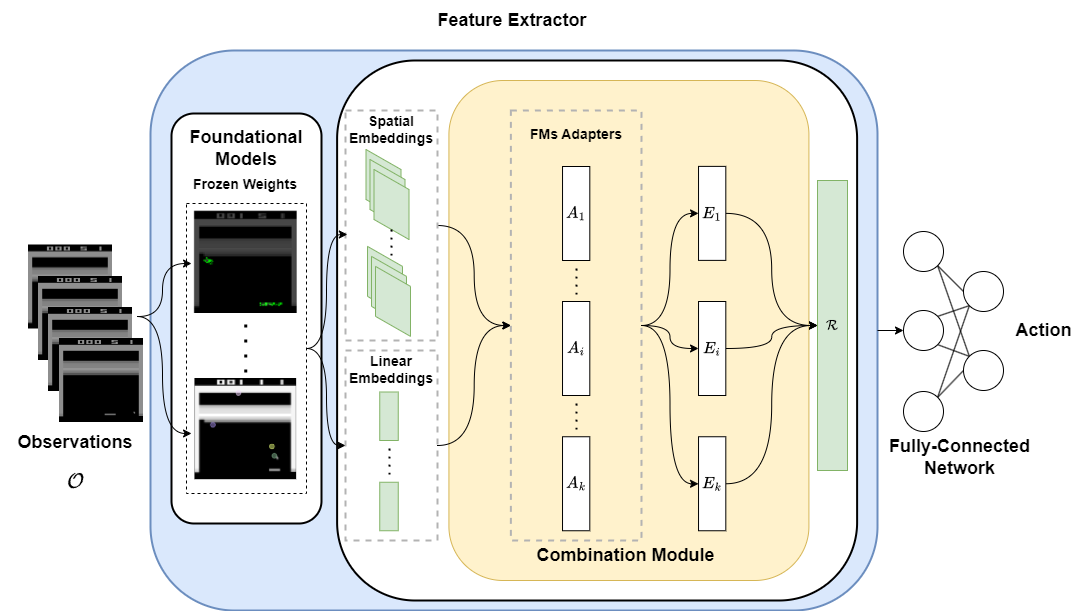
\includegraphics[width=1\textwidth]{images/main_architecture_new}
    \end{center}
    \caption{Figure shows a general representation of the agent's architecture, depicting information flow from observations to actions.
    Last \texttt{4} frames of the game are stacked together to form the observations.
    The Feature Extractor module is responsible for processing the current observation, extracting meaningful representations and combining them.
    It is equipped with a set of pre-trained models and a combination module.
    In general, combination modules are composed by a set of adapters $\mathcal{A}$ which learn a representation of the FM output and eventually resize it a fixed size.
    They produce a set of embeddings $E$ which are then combined in different ways to produce the final representation $\mathcal{R}$.
    The Policy Learning network is the second part of the agent's architecture used to map the current state $\mathcal{R}$ to an action.}
    \label{fig:main}
\end{figure}


In the following sections, we will describe in detail our methodology, and how we map information from observations to actions.
In particular, Sec.~\ref{sec:feature_extractor}, will describe how we designed the Feature Extractor module focusing on various combination techniques to merge the representations extracted by the FMs.
While Sec.~\ref{sec:policy_learning}, we will provide some information about the Policy Learning network.




% prova ad integrare se serve
%Besides our proposed methodology, we tested and compared the performance of several combination modules. All solutions act as interchangable modules inside the \texttt{Feature Extractor}, i.e. only need to replace the \textcolor{orange}{yellow} component in Figure \ref{fig:main_architecture}. Their output is a linear representation that is provided as input to the \texttt{Fully-Connected Network}. We report a rundown across all solutions:
%\begin{itemize}
%    \item \texttt{Linear} (LIN): pre-trained models' representations are linearized and concatenated.
%    \item \texttt{Fixed Linear} (FIX): embeddings are linearized to a predefined size, possibly using adapters to scale the information.
%    \item \texttt{Convolutional} (CNN): FMs' outputs are concatenated along the channel dimension. They are processed by a predefined number of convolutional layers and the resulting information is flattened to linear.
%    \item \texttt{Mixed} (MIX): this is a combination of the previous methods. Data coming from different spaces are dealt separately and then combined.
%    \item \texttt{Reservoir} (RES): inspired by \citet{gallicchio2017}, this approach leverages reservoir layers to combine models' representations.
%    \item \texttt{Dot Product Attention} (DPA): similarly to \texttt{Fixed Linear} the representations are reduced to a specific size - key and value. Via \texttt{scaled dot product attention} \citep{vaswani2017attention} we compute the final weighted representation using as query vector the representation obtained from the State Encoder.
%\end{itemize}




\section{Feature Extractor} \label{sec:feature_extractor}
The Feature Extractor module is the first part of our agent, it is responsible for processing the current observation and extracting a meaningful representation of the environment in a compact latent space.
It is composed itself of two main parts, the first part is a set of pre-trained models, while the second part of the module is the combination module, which is the core of the Feature Extractor.
%a sentence to refer the subsections

\subsection{Foundational Models}\label{subsec:foundational-models}
Agents receive as input the last four frames of the game, which are stacked together to form the observations.
Starting from the observations, the first step of our methodology is to gather information from the environment at different levels of abstraction.
We equipped our agents with a set of $k$ pre-trained models $\Psi = \{\psi_1, \psi_2, \ldots, \psi_k\}$, capable of represent the current observation $\mathcal{O}$ under different perspectives.
Meaning that the models are pre-trained on different tasks.
During the training of RL agents, their weights are frozen in order to preserve the knowledge acquired during the pre-training phase and speed up the learning process.
In particular, we will have a set of $k$ embeddings $E^{FM}$ in output from the FMs, $E^{FM}_i = \psi_i(\mathcal{O})$.
The models operate both in the spatial field, so they output an embedding consisting of a set of feature maps, and in the linear field, so they output a one-dimensional vector.
This is the initial step of our methodology.
We will talk more in detail about the FMs selected in Sec. \ref{sec:exp_setup}.

\subsection{Combination Modules}\label{subsec:combination-modules}
Continuing with the Feature Extractor module, the next step is to combine the representations extracted by the FMs.
Combining different FMs encoding is a challenging task, as each model provides a different view of the environment.
The goal is to merge these perspectives into a single enriched representation that captures the most relevant information.
To achieve this, we developed several combination modules, each with its own strengths and weaknesses.
All solutions act as interchangeable components, and we tested and compared their performance.
All combination modules have in common a first \textit{preprocessing step}, consisting of a set of adapters $\mathcal{A}^{s}$, called \textit{Spatial Adapters}, which are used for embeddings $E^{FM}_i$ that operate in the spatial field.
This set of adapters is implemented as two convolutional layers followed by a ReLU activation function.
This is done to resize the latent representation of the FMs to a fixed size, ensuring compatibility among different models.
While the FMs that operate in the linear field are left as they are.

We will present one by one all the combination techniques that we have developed to merge the representations extracted by the FMs, with a particular emphasis on the Weight Sharing Attention module, which is the component that we propose as a solution to the problem of combining different FMs in an effective way, and we think that it deserves more relevance.
Their output is a linear representation that is provided as input to the \textit{Fully-Connected Network}.

\subsubsection{Weight Sharing Attention}\label{subsubsec:wsa}
With a view to lifelong learning agents, the aim is therefore to equip the agent with prior skills that can be changed or improved over time to adapt to new unseen tasks.
To this end, a model capable of re-adapting to new abilities with little or no effort is needed.
To facilitate the integration of different pre-trained models, we propose WSA\@.
The WSA module leverages the concept of \textbf{weight sharing}, as seen for the first time in CNNs~\citep{fukushima1980neocognitron}, and \textbf{attention}~\citep{vaswani2017attention} principles to efficiently merge outputs from diverse FMs.
In specific, WSA dynamically adjusts the weights assigned to each pre-trained model based on the current context, emphasizing the most relevant models for the current state.

This module, depicted in Fig. \ref{fig:wsa_main_architecture}, is designed in this way.
It receives as input the representation extracted by the FMs, on which it applies the preprocessing step described before.
Then, spatial embeddings are flattened to obtain a one-dimensional vector.
WSA module is equipped with another set of adapter, called \textit{Linear Adapters} $\mathcal{A}^{l}$, where each adapter $\mathcal{A}^{l}_i$ is a small neural network consisting of a single linear layer followed by a non-linearity layer, in this case, a ReLU activation function.
The adapters are used to learn a representation of FMs output and also to resize the different linear latent representations of the state to a fixed size.
This guarantees consistency between various models.
As a result of this operation, we obtain an embedding for each FM representation, called $E^{l}_i$.
All the embeddings have the same dimension, and it is possible to combine them in a meaningful way.


\begin{figure}[ht]
    \begin{center}
        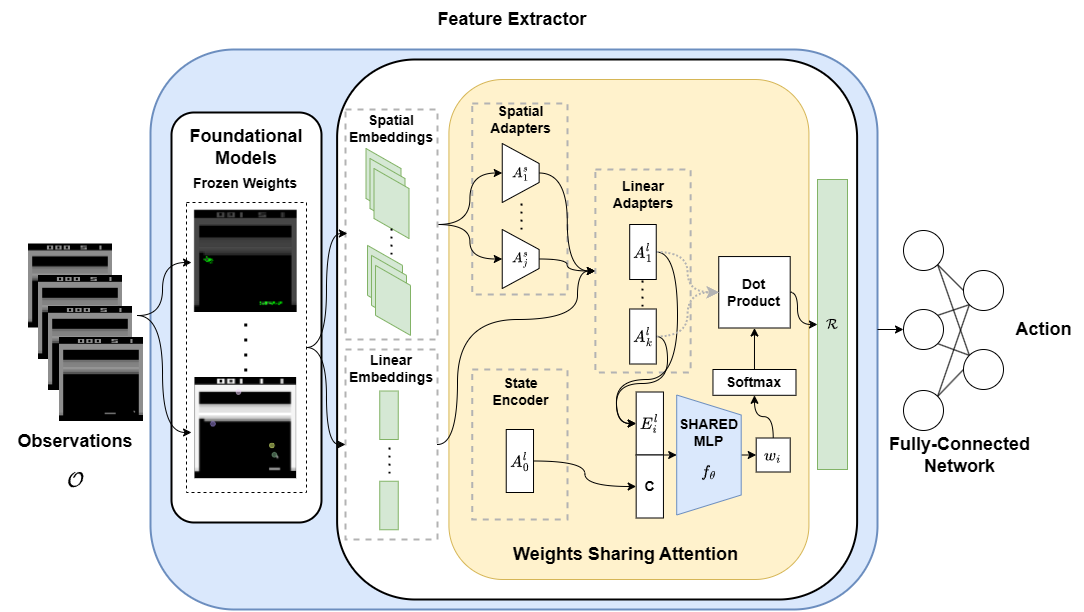
\includegraphics[width=1\textwidth]{images/wsa_main_architecture}
    \end{center}
    \caption{In Figure, we show in specific all the information course from game frames to agent actions specifying the architecture of the WSA module. The last four frames are stacked together and passed as input to the FMs and their spatial adapters $\mathcal{A}^{s}_1, \dots \mathcal{A}^{s}_j$ first, and then to the linear adapters $\mathcal{A}^{l}_1, \dots \mathcal{A}^{l}_k$ to obtain an embedding of the current state $E^l_i$. A State Encoder $\mathcal{E}$ and its adapter $\mathcal{A}^l_0$ compute an encoding of the state, that will be used as context $\mathcal{C}$. A shared MLP layer takes as input the context $\mathcal{C}$ and the representation of the $i^{th}$ FM, $E^l_i$, and produces the weight $w_i$ for that specific view of the state. The final enriched representation $\mathcal{R}$ is obtained from the weighted summation between each weight $w_i$ and its respective embedding $E^l_i$. $\mathcal{R}$ is given as input to agents' \textit{Fully-Connected Network}.}
    \label{fig:wsa_main_architecture}
\end{figure}


Among the provided FMs, one is used as \textbf{State Encoder} $\mathcal{E}$ to compute a representation of the current state, which serves as \textit{context} $\mathcal{C}$ for the attention mechanism.
The State Encoder produces a spatial encoding of the current observation which is flattened to obtain a linear embedding.
A linear adapter $\mathcal{A}^{l}_0$, of the same shape of the other linear adapters, is used to resize the latent representation to a fixed size, and this will be the context $\mathcal{C}$.

To compute the attention weights, we use a shared MLP $f_\theta$ that takes as input the context $\mathcal{C}$ concatenated with the single embedding $E^{l}_i$ of each FM\@.
This MLP outputs the model-specific weight $w_i$ to determine the contribution of each model in the final representation.
Weights are stacked together and passed through a softmax function to ensure that they sum to one.
It is important to note that this MLP is shared across all models, ensuring uniform weight computation.
By dynamically adjusting weights based on the current context, WSA emphasizes the most relevant models for any given situation, resulting in a more accurate and adaptable representation.
The final representation $\mathcal{R}$ is computed using the weights for all pre-trained models and computing a weighted sum of their embeddings.
The output obtained is so a combination of the various perspectives, provided by the pre-trained models, into a single enriched latent representation.
This final linear representation is used for action mapping, enhancing the performance and learning efficiency of RL agents by integrating the strengths of multiple FMs.
The weights of the adapters are optimized during training.

Two additional features are guaranteed by the design approach.
WSA adds \textbf{explainability} to the model, where with explainability we mean the ability to understand the decision-making process of the agent.
In fact, by examining the weights assigned to different pre-trained models, we can gain insights into which models are most influential in a given context.
Additionally, WSA is \textbf{scalable} and \textbf{adaptable} to any number of pre-trained models.
Its shared component can handle any number of models, we can easily add or remove FMs from the set without the need to retrain the whole agent, making it a flexible solution for dynamically evolving agents.
Algorithm~\ref{alg:wsa} reports the pseudocode for the actual implementation.

\begin{algorithm}[ht]
    \caption{Weight Sharing Attention}\label{alg:wsa}
    \texttt{In \textcolor{blue}{blue} we highlight the components that are updated during training.}\\
    \begin{algorithmic}[1]
        \Require Current observation $\mathcal{O}$, List of FMs $\Psi$, State Encoder $\mathcal{E}$
        \State $\mathcal{C} = \textcolor{blue}{\mathcal{A}_0}(\mathcal{E}(\mathcal{O}))$ \Comment{Compute current context representation}
        \For {FM $\psi$ in $\Psi$}
            \State $x = \psi_i(\mathcal{O})$ \Comment{Forward pass using current state}
            \State $E_i = \textcolor{blue}{\mathcal{A}_i}(x)$ \Comment{Use the adapters to compute the resized embedding}
            \State $w_i = \textcolor{blue}{f_\theta}(\mathcal{C}, E_i)$ \Comment{Compute the weight for current model using shared component}
        \EndFor
        \State $\mathcal{R} = \sum_{i=0}^{|\Psi|} w_i * E_i$ \Comment{Final representation: weights $W$, embeddings $E$ $\rightarrow$ $W \cdot E$}
    \end{algorithmic}
\end{algorithm}





\subsubsection{Linear Combination Modules}\label{subsubsec:linear_combination}
Linear combination modules are the simplest way to merge the representations extracted by the FMs.
Considering the set of $k$ pre-trained models, each of them can output an embedding in the spatial field or a one-dimensional vector.
We apply the spatial adapters to the embeddings that operate in the spatial field, and we leave the linear embeddings as they are.
Then, we flatten the spatial embeddings to obtain a linear encoding.
The embeddings of each model are then concatenated to create a large feature vector.
This constitutes the final representation of the environment $\mathcal{R}$.
We refer to this module as \textit{LIN} for short.

Building such a large vector can be helpful since the information from different models are not compressed, and the final representation is rich and informative.
One problem though with this combination module is that the FMs may have very different dimensionality.
An embedding might be huge compared to the others, leading to a situation where one model becomes more important than the others just because its dimension is larger.
So, we developed another combination module, which we refer to as \textit{FIX}, where first we obtain a linear representation as in the previous module for each model.
Then, we map the representation of each model into an embedding of fixed dimensions using $k$ linear adapters $\mathcal{A}^{l}$ of the same size.
Each adapter is a neural network constituted of a linear layer is followed by a ReLU activation function.
The new embeddings $E^{l}$ are then concatenated as before to compute the representation $\mathcal{R}$ and used as input for the rest of the network.
In Fig.~\ref{fig:lin_combination} we show the architecture of the two linear combination modules.


\begin{figure}[ht]
    \centering
    \begin{subfigure}[b]{0.49\textwidth}
        \centering
        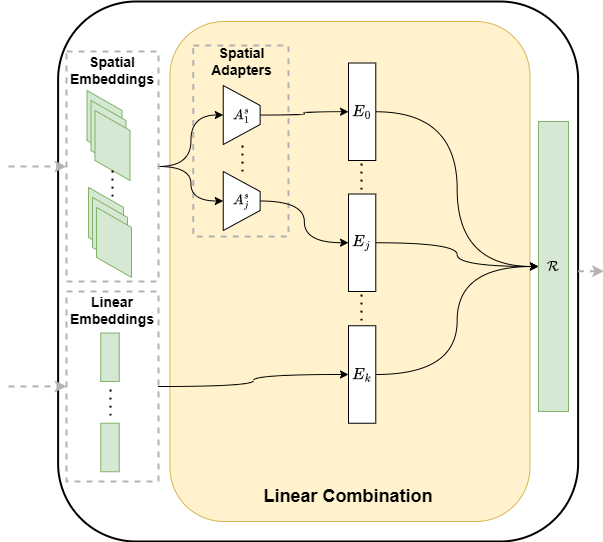
\includegraphics[width=\textwidth]{images/lin}
        \caption{\texttt{LIN}}
        \label{fig:lin}
    \end{subfigure}
    \hfill
    \begin{subfigure}[b]{0.49\textwidth}
        \centering
        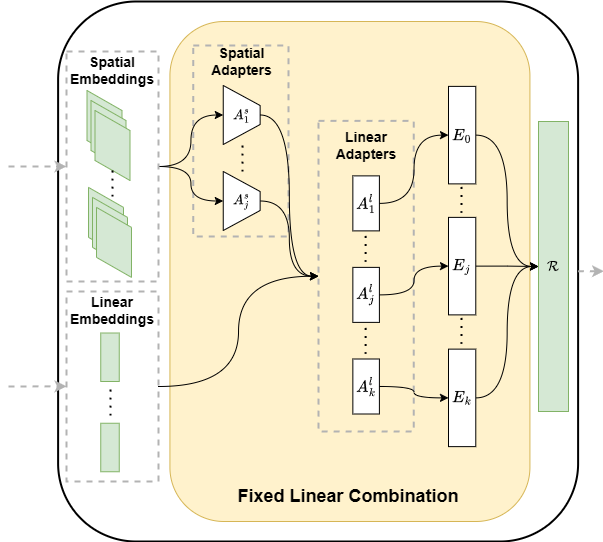
\includegraphics[width=\textwidth]{images/fix}
        \caption{\texttt{FIX}}
        \label{fig:fix_lin}
    \end{subfigure}

    \caption{In Figure we show the architecture of the Linear Combination Module (LIN) and the Fixed Linear Combination Module (FIX). In LIN, the embeddings of each model are first flattened to one-dimensional vectors, then concatenated to create a large feature vector. In FIX, the embeddings are also mapped into encodings of fixed dimensions using $k$ different linear layers with the same size and then concatenated}
    \label{fig:lin_combination}
\end{figure}




\subsubsection{Convolutional Combination Modules}
\label{subsubsec:convolutional_combination}
In this combination module, we exploit the fact that FMs operate in the spatial field.
In fact, flatting the feature maps and concatenating them as in the linear combination modules may not be the best choice, as the spatial information is lost.
To overcome this issue, after applying the usual preprocessing step consisting of the spatial adapters, we reshaped the one-dimensional embeddings into spatial ones, to match the dimensions of the other representations.
Then, the embeddings are \textbf{concatenated along the channel dimension} and passed to one or more convolutional layers $\mathcal{A}^c$ to extract features.
At this point, the output of the convolutional layer is flattened to constitute the final representation $\mathcal{R}$, and the embedding is passed to the rest of the network.
We refer to this combination module as \textit{CNN}.

This module is particularly useful when the FMs are designed to capture spatial information, as in the case of images, but there may be cases where the FMs are not designed to capture spatial information.
Assuming that the set of FMs is composed of models that operate in the spatial field and models that operate in the linear one, we can exploit these two types of models to create a more complex combination module.
As before, first we preprocess the output of the FMs using the spatial adapters.
Then, we concatenate the FMs embedding that operate in the spatial field along the channel dimension.
We then pass this embedding through a single convolutional layer to extract spatial features, followed by a ReLU activation function.
Finally, we flatten the output of the convolutional layer and concatenate it with the embeddings of the linear FMs to create the final representation $\mathcal{R}$.
We call this combination module \textit{MIX} as it is a mixture of the previous two modules.

Figure~\ref{fig:conv_combination} shows the architecture of the two convolutional combination modules.

\begin{figure}[ht]
    \centering
    \begin{subfigure}[b]{0.49\textwidth}
        \centering
        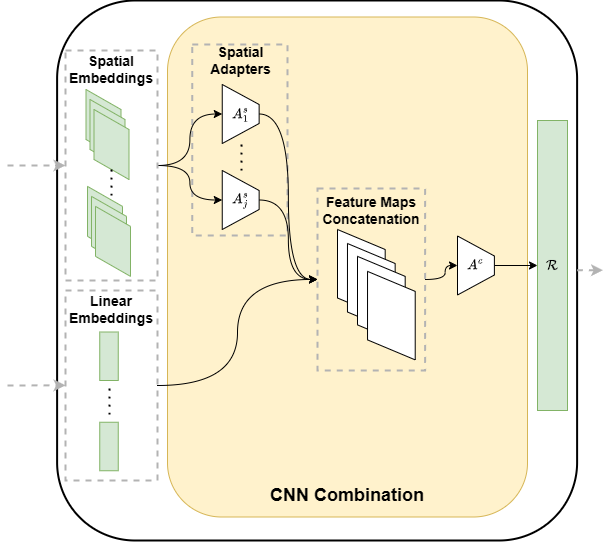
\includegraphics[width=\textwidth]{images/cnn}
        \caption{\texttt{CNN}}
        \label{fig:cnn}
    \end{subfigure}
    \hfill
    \begin{subfigure}[b]{0.49\textwidth}
        \centering
        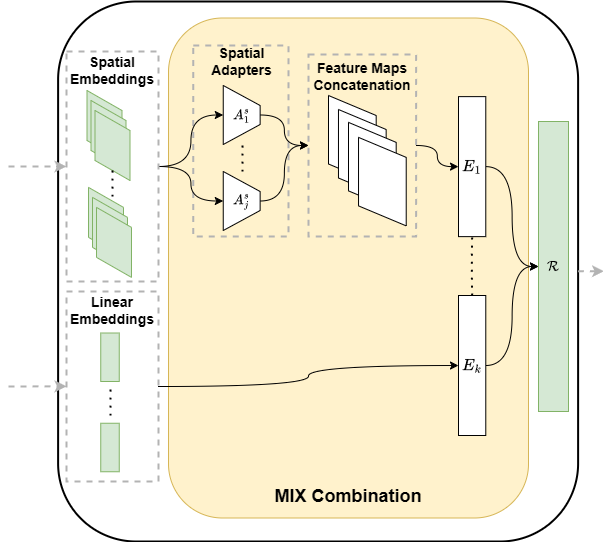
\includegraphics[width=\textwidth]{images/mix}
        \caption{\texttt{MIX}}
        \label{fig:mix}
    \end{subfigure}

    \caption{n Figure we show the architecture of the Convolutional Combination Module (CNN) and the Mixed Combination Module (MIX). In CNN, we first reshape all embedding such that can be concatened along the channel dimension. Then we use a CNN to extract feature and produce the representation $\mathcal{R}$. In MIX, first we concatenate the spatial embeddings together, then we flatten their representaion to a linear one and concatenate all the linear embeddings.}
    \label{fig:conv_combination}
\end{figure}

\subsubsection{Reservoir Combination Module}
\label{subsubsec:reservoir_combination}
Inspired by the work of \citet{gallicchio2017}, we decided to explore reservoir dynamics properties to map the input into a lower-dimension latent space using a non-linear transformation.
To develop this combination module, we created a \textit{reservoir} with fixed weights using a predefined number of neurons.
As input, for the reservoir we used the representation $\mathcal{R}$ built by the LIN combination module.
The output of the reservoir is a vector of the size of the number of neurons on it.
This is the new computed representation $\mathcal{R}$, which is used as input to the policy learning network, which can be viewed as the \textit{readout}.
We refer to this combination module as \textit{RES}.
Figure~\ref{fig:reservoir_combination} shows the architecture of the reservoir combination module.

\subsubsection{DotProduct Attention Combination Module}
\label{subsubsec:dpa}

We also explored the possibility of combining representations using different types of attention-like mechanisms conditioned on the configuration of the environment.
In this case, we used the \textit{scaled dot product attention}~\citep{vaswani2017attention}.
As for the WSA module, the pre-trained model representations are reduced to a vector of fixed size using the spatial and linear adapters.
These are then stacked together to form a tensor of shape $(k \times \text{vector\_size})$, where $k$ are the number of available FMs, and $vector\_size$ is the fixed dimension of each pre-trained model embedding.
This constitutes the \textbf{key} part and the \textbf{value} part of the attention module.
For the \textbf{query} part, we used the same procedure as for the WSA module to produce the context $\mathcal{C}$.
We used the State Encoder to encode the current state of the game in a latent space, and we used an adapter to obtain a vector of the same dimensions.
As the name of the module suggests, the attention module first computes the dot product of the query with the keys, divided by the square root of the dimension of the query, then it uses a softmax function to obtain the weights.
Finally, the output of the module is computed as the dot product of the weights with the values.
We call this combination module \textit{DPA} and in Fig.~\ref{fig:dpa_combination} we show the architecture of the module.


\begin{figure}[ht]
    \centering
    \begin{subfigure}[b]{0.49\textwidth}
        \centering
        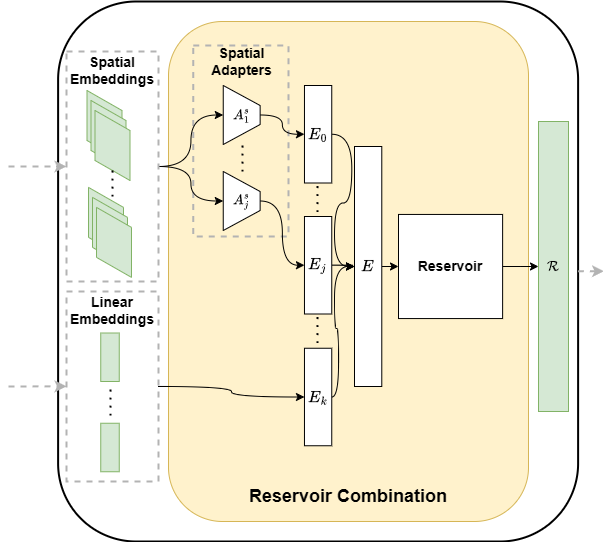
\includegraphics[width=\textwidth]{images/res}
        \caption{\texttt{RES}}
        \label{fig:reservoir_combination}
    \end{subfigure}
    \hfill
    \begin{subfigure}[b]{0.49\textwidth}
        \centering
        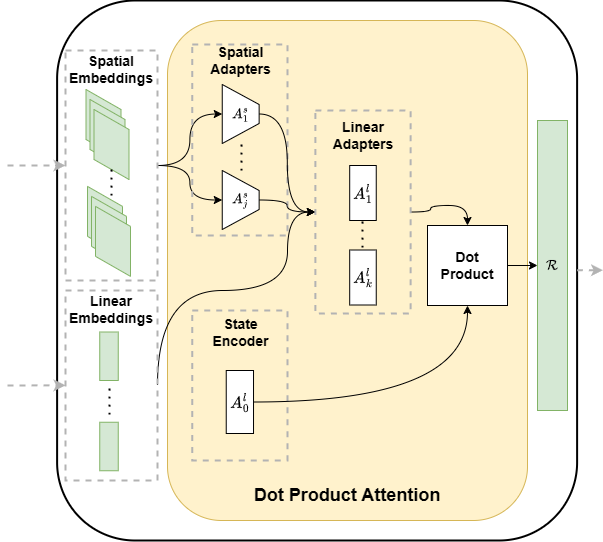
\includegraphics[width=\textwidth]{images/dpa}
        \caption{\texttt{DPA}}
        \label{fig:dpa}
    \end{subfigure}

    \caption{n Figure we show the architecture of the Reservoir Combination Module (RES) and the DotProduct Attention Combination Module (DPA). In RES, we use reservoir dynamics to encode information coming from different FMs. In DPA, the embeddings are mapped into an embedding of fixed dimensions using $k$ different linear layers with the same size and we use the State Encoder $\varepsilon$ as context $\mathcal{C}$, as for WSA.}
    \label{fig:dpa_combination}
\end{figure}



\section{Policy Learning}\label{sec:policy_learning}
This is the last part of the agent's architecture, where the enriched representation obtained from the Feature Extractor module is used to map the current state to an action.
It receives as input the augmented representation $\mathcal{R}$ as a one-dimensional vector.
$\mathcal{R}$ is assumed to contain all the relevant information, simplifying the learning process of the agent.
The Policy Learning network is a small fully-connected neural network that takes as input $\mathcal{R}$ and outputs the probability distribution over the possible actions or the value function.
The network generally is composed of just one layer with a small number of neurons.
Eventually, the size of this network can be increased to capture more complex dynamics and to improve the performance of the agent by increasing the number of layers and adding non-linearity functions between them.

%! Author = giaco
%! Date = 16/05/2024

\chapter{Experiments \& Results}
\label{ch:experiments_and_results}
In this chapter, we are going to provide information about how we implemented the various modules of our work, the experiments that we conducted to test our agents, and the results obtained.
We start by describing the experimental setup in Sec. \ref{sec:exp_setup}, talking about the libraries and tools used, the data collected, the training process, and the environments used to evaluate our agents.
We will present the experiments we performed one by one and for each one, we will show the results obtained.
We start from the initial experiments in Sec. \ref{sec:init_exp}, where we tested different combination modules to find the best-performing ones.
Then, in Sec. \ref{sec:top-3-performer}, we will consider only the best three performing modules for each game, and we will compare them with PPO\@.
In Sec. \ref{sec:breakout_study}, we will focus on the \textit{Breakout} game, which showed a different behavior compared to the other games.
We will analyze the reasons behind this behavior and propose some possible solutions to improve the performance of the agent in this game.
In Sec. \ref{sec:explainability}, we will provide an explanation of the Weight Sharing Attention mechanism and how it works.
Finally, in Sec. \ref{sec:dqn}, to prove that our approach is not dependent on the RL algorithm used, we will test the effectiveness of WSA  using \textbf{DQN}.

\section{Experimental Setup}\label{sec:exp_setup}
In order to interact and simulate Atari environments~\citep{bellemare2013atari} we used broadly the API provided by Gymnasium~\citep{towers_gymnasium_2023}, which has extensive support for Atari games and has been widely used in the RL community.
The training performance was tracked using \textit{Weights and Biases}~\citep{wandb}, which is a machine learning platform that provides tools for experiment tracking, model optimization, and more.
The platform allows to monitor the agents and store the results in a cloud-based database.

Our work uses \textit{Stable-Baselines3} (SB3)~\citep{stable-baselines3} as a framework for agent architecture and reliable implementations of RL algorithms in PyTorch.
SB3 implements the algorithms with a modular architecture, which allows to easily modify the agent's structure.
This is particularly useful for us, as we need to combine different representations in the agent's architecture.
In fact, SB3 provides a simple interface to decompose the agent's network into a \textit{Feature Extractor} and a \textit{Fully-Connected Network}, and this is the schema that we reported in our architecture as shown in Figure~\ref{fig:main}.
We used the \textit{Feature Extractor} to implement the different combination modules providing as output the composed latent representation.
The \textit{Fully-Connected Network} is kept as simple as possible, this is because most of the information should be provided by the FMs' representations.
It receives as input the FMs' combined linear encoding and subsequently maps it to actions (or values).

For our experiments, we mainly used PPO algorithm~\citep{schulman2017proximal} as it is one of the most widely used algorithms in the RL community.
We maintained the hyperparameters provided by \citet{rl-zoo3} for PPO.
We did not conduct any hyperparameter search this time, this to avoid adding complexity to the experiments and growing the time.
Instead, we only modify the model architecture.
Table~\ref{tab:ppo_hyperparams} shows the hyperparameters used for the PPO agent.

\begin{table}[htbp]
    \centering
        \begin{tabular}{ll}
            \multicolumn{1}{l}{\bf Hyperparameter}  &\multicolumn{1}{l}{\bf Value}
            \\ \hline \\
            N. Envs.       & 8 \\
            N. Stacks      & 4 \\
            N. Steps       & 128 \\
            N. Epochs      & 4 \\
            Batch Size     & 256 \\
            N. Timesteps   & 10.000.000 \\
            Learning Rate  & 2.5e-4 \\
            Clip Range     & 0.1 \\
            VF. Coef.      & 0.5 \\
            Ent. Coef.     & 0.01 \\
            Normalize      & True \\
        \end{tabular}
        \caption{PPO hyperparameters.} \label{tab:ppo_hyperparams}
\end{table}

To set the environment in order to be used by the agent, we used the \textit{Atari Preprocessing} wrapper provided by SB3, which preprocesses the frames by grayscaling them, resizing them to 84x84 pixels, and then stacking the last four frames to provide the agent with temporal information.
We also run multiple instances of the environment in parallel to speed up the training process, in particular, we used \texttt{8} parallel environments.
So, the agent receives as input a tensor of shape $8 \times 4 \times 84 \times 84$, where the first dimension represents the number of parallel environments, the second dimension represents the number of frames stacked together and the last two dimensions represent the size of the frame.
The experiments were conducted on a machine equipped with 4 Intel Xeon Gold 6140M CPUs for a total of 144 threads, 4 Nvidia Tesla V100 GPUs with 16GB of memory, and 1.2TB of RAM\@.
The experiments were conducted on a single GPU, eventually running multiple experiments in parallel.


\subsection{Environments}
\label{subsec:environments}
In this section, we provide a brief overview of the environments used to evaluate our agent.
We have chosen a set of Atari games that are widely used in the literature to evaluate their performance.
We focused on games that have a discrete action space and discrete observations.
In particular, we have selected games that require different skills to be solved, in order to test the effectiveness of our agent in a variety of tasks.
We will list the games used in the experiments, and we will provide a brief description of each one.
In Fig.~\ref{fig:environemnts} we provide an example of game frames for each one.
\subsubsection{Pong}
The game of Pong is a table tennis simulation.
This game is played by two players, each controlling a paddle that can move up and down along the left and right edges of the screen.
The paddles are used to hit a ball back and forth.
The right paddle is controlled by the RL agent, while the left paddle is controlled by the opponent.
Points for a player are accumulated when the opponent is unable to successfully return the ball, resulting in the ball passing beyond their paddle.
The objective of the game is to score as many points as possible preventing the opponent from doing the same.
The game ends when one of the players reaches the score of \texttt{21}.
From the viewpoint of the RL agent, the game is considered solved when it is able to consistently outperform the opponent.


\subsubsection{Breakout}
Breakout is a game where the dynamic is similar to Pong, but the objective is different.
In this case, the environment is constituted by a paddle that can move horizontally at the bottom of the screen, which hits a ball that bounces on the walls.
At the top of the screen, there is a wall of bricks, and the agent has to break them using the ball that bounces on the paddle.
The more bricks the agent breaks, the higher the score it gets.
When the agent breaks all the bricks the environment is reset and the agent can start a new game.
When the agent fails to intercept the ball, it loses one life, and when it loses all lives, it loses the game.
Again, the goal of the game is to score as many points as possible.


\subsubsection{Ms. Pacman}
This game is a maze game where the agent controls a character that moves through the environment and collects various objects.
The objects are represented by dots, fruits, or power pellets that are scattered throughout the maze.
The agent navigates the maze searching for dots, the more dots the agent collects, the higher the score it gets.
Various fruits and other bonus items appear in the maze at certain times.
Eating these items grants additional points.
The agent also has to avoid the ghosts that move through the maze, as they can kill the agent.
The only way to kill the ghosts is to eat power pellets that appear in the maze from time to time and give the agent the ability to eat the ghosts.
Eating ghosts also grants additional points.
The game ends when the agent loses all its lives, or when it collects all the dots in the maze. 
\begin{figure}[ht]
    \centering
    \begin{subfigure}[b]{0.30\textwidth}
        \centering
        \fbox{\rule[-.5cm]{0cm}{4cm} \rule[-.5cm]{4cm}{0cm}}
        %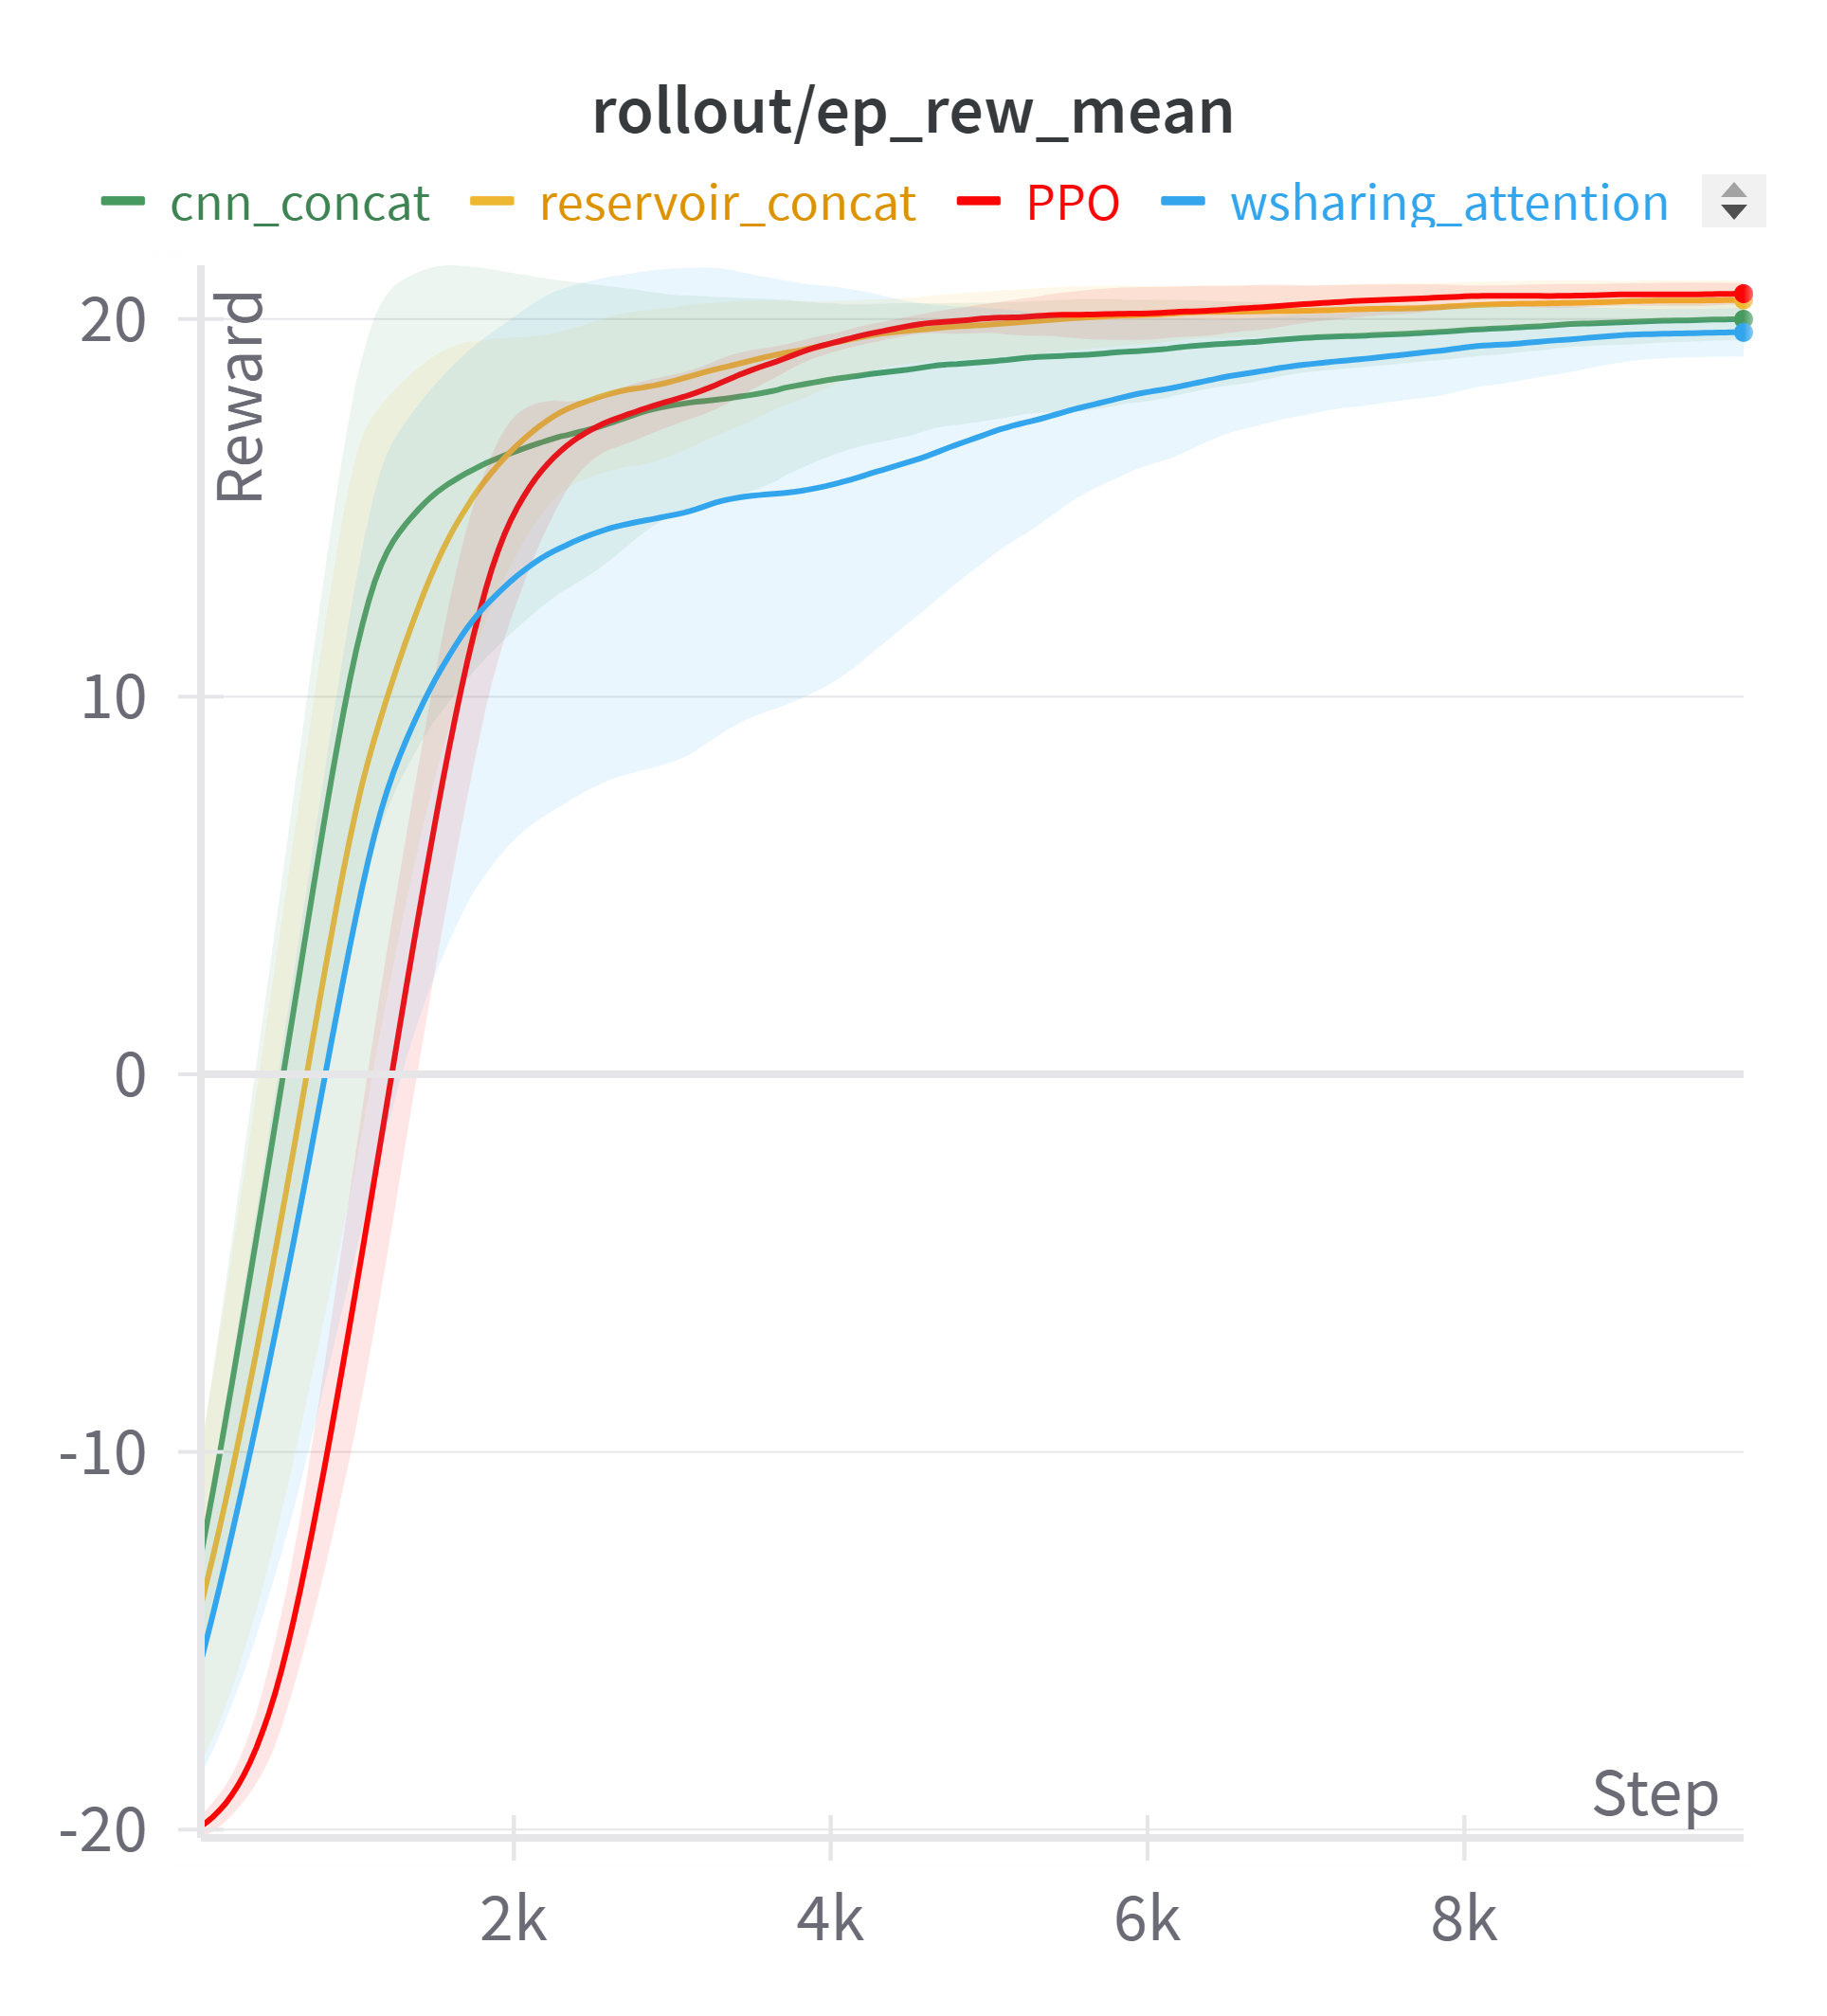
\includegraphics[width=\textwidth]{images/pong_train.png}
        \caption{\texttt{Pong}}
        \label{fig:pong_env}
    \end{subfigure}
    \hfill
    \begin{subfigure}[b]{0.30\textwidth}
        \centering
        \fbox{\rule[-.5cm]{0cm}{4cm} \rule[-.5cm]{4cm}{0cm}}
        %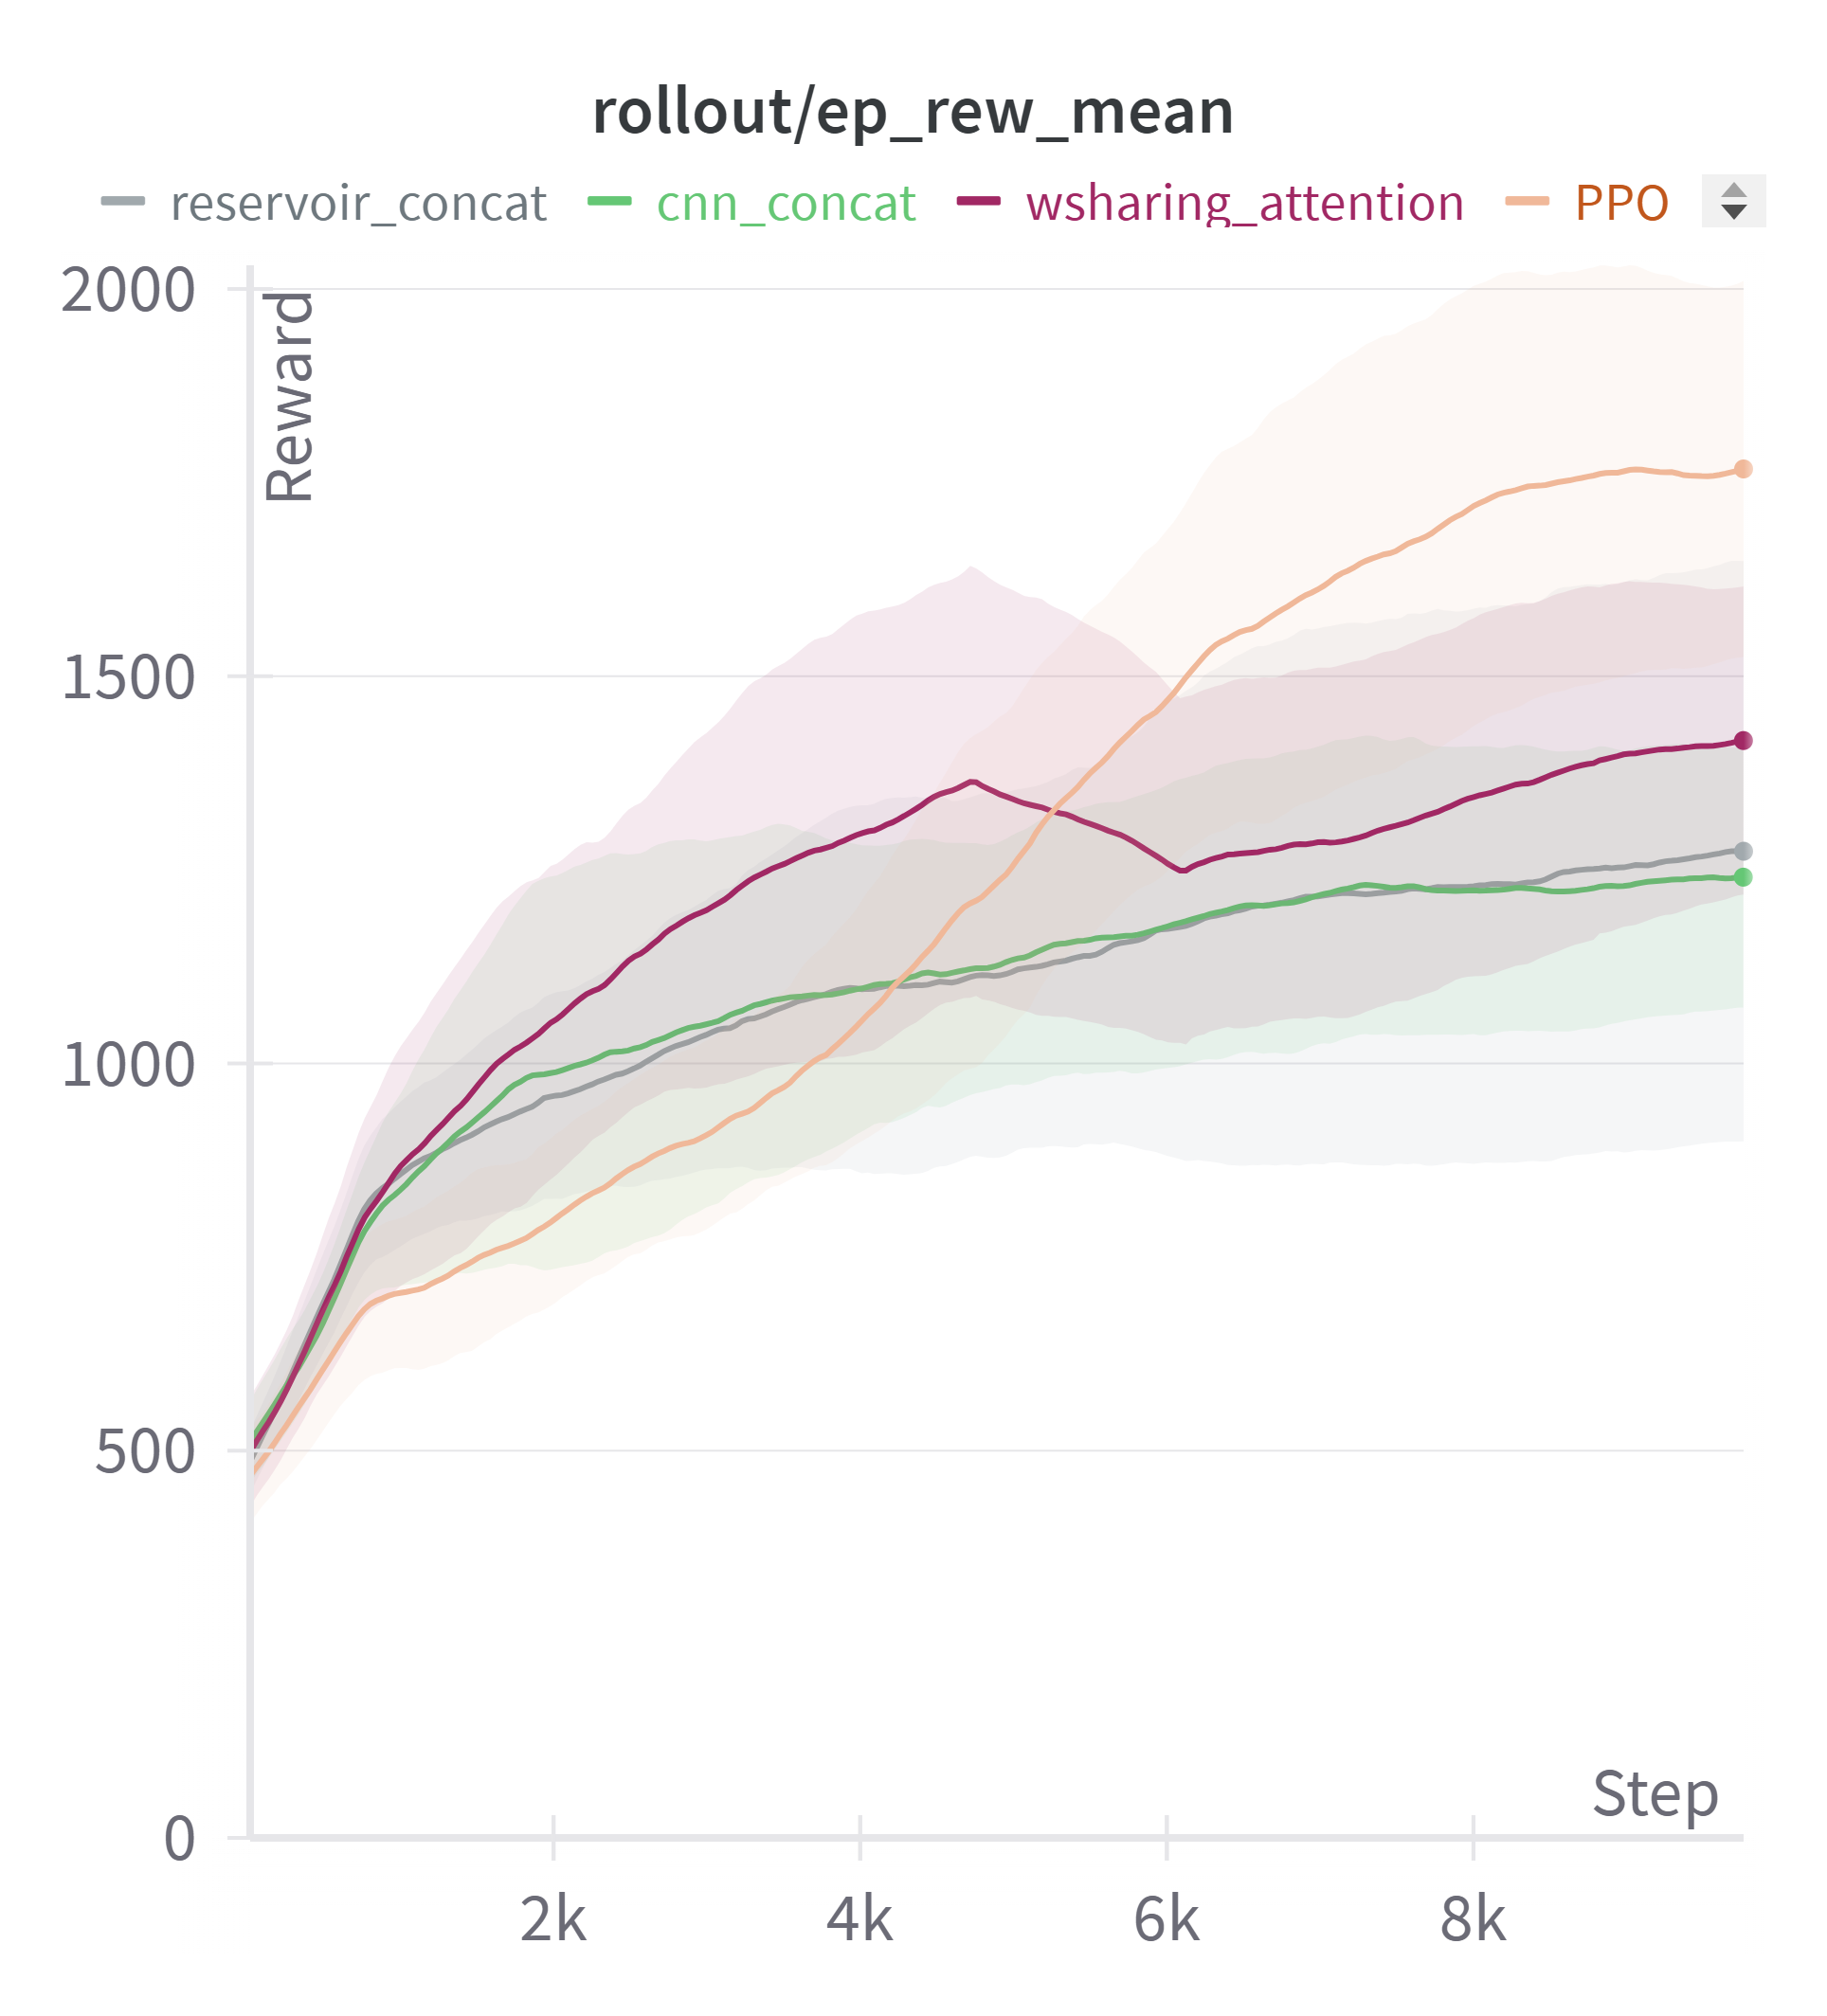
\includegraphics[width=\textwidth]{images/mspacman_train.png}
        \caption{\texttt{Ms.Pacman}}
        \label{fig:mspacman_env}
    \end{subfigure}
    \hfill
    \begin{subfigure}[b]{0.30\textwidth}
        \centering
        \fbox{\rule[-.5cm]{0cm}{4cm} \rule[-.5cm]{4cm}{0cm}}
        %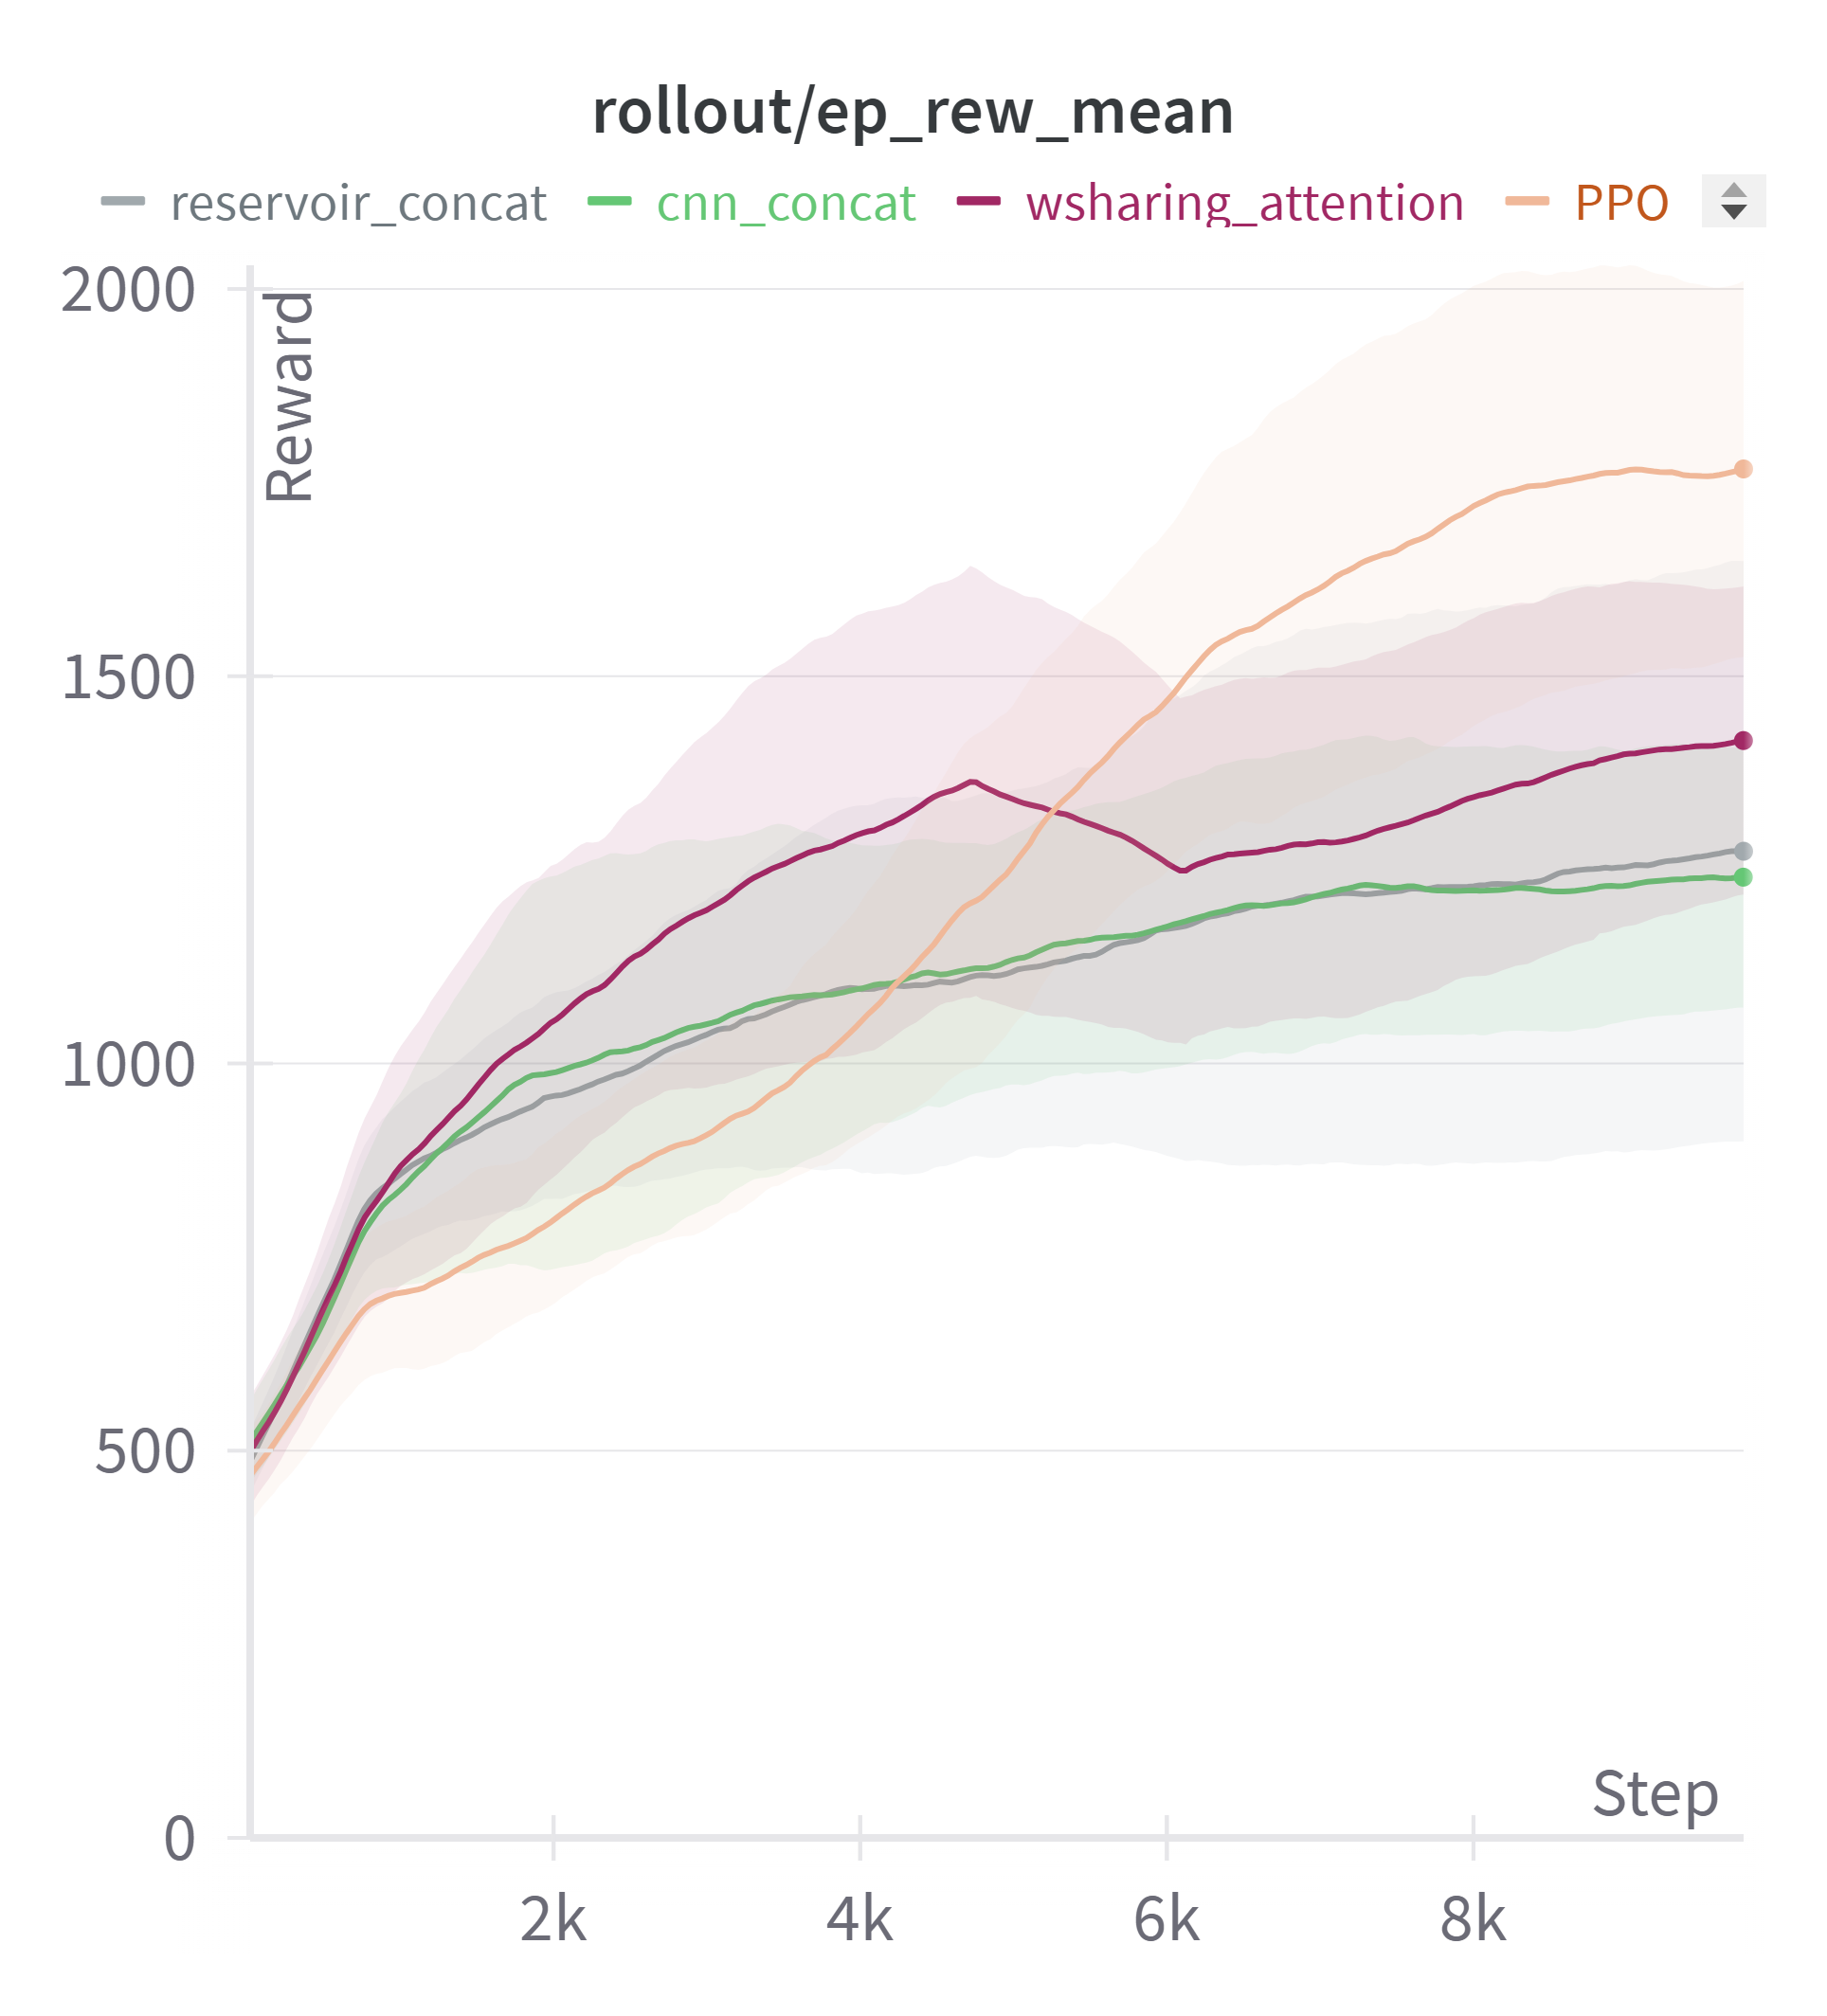
\includegraphics[width=\textwidth]{images/mspacman_train.png}
        \caption{\texttt{Breakout}}
        \label{fig:breakout_env}
    \end{subfigure}
    \caption{A snapshot of the environments}
    \label{fig:environemnts}
\end{figure}


\subsection{FMs Data and Training}\label{subsec:fms-data-and-training}
For the main experiments of our approach, we use three different models which provide us with four different pre-trained networks: \textit{Video Object Segmentation} (VOS)~\citep{goel2018unsupervised}, \textit{State Representation} (SR) \citep{anand2019unsupervised}, and finally \textit{Object Keypoints}~\citep{kulkarni2019unsupervised} which provides us the object encoder (OKE) and the object keypoint network (OKK).
These models constitute the set of basic skills that the agent is equipped with.
We believe that these models provide a good starting point for the agent to learn the environment, and they are informative enough to provide a good representation of the state.
In fact, SR gives a general representation of the state in a compact form, VOS tracks moving objects in the frame which can be useful for tracking the ball in Pong or Breakout or the ghosts in Ms.Pacman, and finally, Object Keypoints provides the agent with the position of the objects in the frame.

Additionally, for attention-based combination modules, we train a deep autoencoder - inspired by Nature CNN~\citep{mnih2015human} - to encode the current state and leverage its representation to compute the context.
The architecture of Nature CNN has been slightly modified as it appears in Tab. \ref{tab:nature_cnn} to
match the dimensions of other FMs' representations.

\begin{table}[htbp]
     \begin{center}
         \begin{tabular}{lllll}
             \multicolumn{1}{l}{\bf Layer}  & \multicolumn{1}{l}{\makecell{\bf In.\\\bf Channels}}  & \multicolumn{1}{l}{\makecell{\bf Out.\\\bf Channels}}  & \multicolumn{1}{l}{\makecell{\bf Kernel\\\bf size}}  & \multicolumn{1}{l}{\bf Stride}
             \\ \hline \\
             1st CNN Layer   &  1  & 32 & 8 & 4 \\
             2nd CNN Layer   &  32  & 64 & 3 & 1 \\
             3rd CNN Layer   &  64  & 64 & 3 & 1 \\
         \end{tabular}
     \end{center}
     \caption{This table shows the encoder architecture of the Deep Autoencoder. It takes as input only the last frame in grayscale. The stride on the second convolutional layer was decreased from 2 to 1 with respect to Nature CNN. Each convolutional layer is followed by a ReLU activation function. The decoder part is specular.}
     \label{tab:nature_cnn}
 \end{table}




To train the different FMs and the Autoencoder we first create a specific dataset for each game.
For each environment, we collected \texttt{1M} frames via agents interacting with the environment.
The agents act randomly in this case, and the frames are collected without any reward.
This is done to ensure that the data is not biased towards a specific policy.
The dataset contains grayscale game frames with a size of 84x84 pixels.
During the training process of the models, game frames are randomly sampled to avoid any correlation between elements due to the collection phase since the frames are collected sequentially.
We implemented and trained the models for all the games using the default architecture and hyperparameters provided by the authors.
The values and additional details are reported in Appendix~\ref{sec:app-models}.
While training the agent, pre-trained models' weights are frozen and no longer updated.

It is important to note that we build a model for each game, and we do not use a single model for all the games.
These FMs are small models that can be easily changed to more complex models without affecting the structure of our work if needed.


\section{Initial Experiments}\label{sec:init_exp}
As shown in Section~\ref{subsec:environments}, we chose three different Atari games as benchmarks for our work, namely \textit{Pong, Breakout, and Ms. Pacman,}
The first choice of the games was dictated by the availability of the RAM annotations provided in~\cite{anand2019unsupervised}.
Then to avoid adding complexity and growing the time for experiments we restricted to testing only the games already cited.
We believe that this choice of games provides a fair compromise between simple games like \textit{Pong} and much more complex games with many moving parts like \textit{Pacman}.
For each environment, we selected the \textit{NoFrameskip-v4} version of the game which is the most common version used in the literature. 
In this version, the agent can take an action in every frame.

After training each FM, we ran a first round of experiments using the three games, where we implemented the \textit{Feature Extractor} using all the combination modules shown in Section~\ref{sec:feature_extractor} one at a time with different embedding sizes or configurations.
The \textit{Fully-Connected Network} is set to a single layer of \texttt{256} units both for policy network and value function network.
As shown in Table~\ref{tab:emb_siz_modules}, we explore a variety of configurations for each module, ensuring a comprehensive assessment of their performance.

\begin{table}[ht]
    \begin{center}
        \begin{tabular}{ll}
            \multicolumn{1}{l}{\bf Feature Extractor}  &\multicolumn{1}{l}{\bf Embedding Size}
            \\ \hline \\
            LIN              &  - \\
            FIX        & 256, 512, 1024 \\
            CNN       & 1, 2, 3\\
            MIX                             & - \\
            RES           & 512, 1024, 2048 \\
            DPA             & 256, 512, 1024 \\
            WSA         & 256, 512, 1024 \\

        \end{tabular}
    \end{center}
    \caption{The table shows all the extractors' configurations tested in the initial phase of experiments. For FIX, DPA, and WSA the values indicate the fixed dimensions of embeddings and context, for RES the size of the reservoir and for CNN the number of convolutional layers.}
    \label{tab:emb_siz_modules}
\end{table}


This first phase of experiments aims to find the \texttt{3} best-performing combination modules that will be used for our empirical analysis along with our proposed method.
Agents are trained for \texttt{10M} steps using the parameters provided by \texttt{rl-zoo}, and throughout the learning process, agents are repeatedly evaluated each \texttt{40.000} for \texttt{100} episodes.
During the training phase of these first experiments, we applied \textbf{early stopping} for agents that showed no improvement over \texttt{5} consecutive evaluations.
This strategy allowed us to promptly identify the best-performing configurations and to save computational resources as these experiments are computationally expensive.
In Appendix~\ref{sec:app-com-mod} we report all the learning curves in this experimental phase.

Here instead we show our first results providing the best-performing modules for each game, the chosen embedding size is detailed between parentheses:
\begin{itemize}
    \item \texttt{Pong}: WSA (1024), RES (1024), CNN (2)
    \item \texttt{Ms.Pacman}: WSA (256), RES (1024), CNN (2)
    \item \texttt{Breakout}: WSA (256), FIX (512), CNN (3)
\end{itemize}

\section{Top 3 Performer}\label{sec:top-3-performer}
In the subsequent phase, the research progressed with a refined focus.
We used the same methodology and setup as the initial experiments for our empirical evaluation, but we restricted the tests only to the best-performing modules for each game.
This time we avoid using early stopping, and we let the agents train for the full \texttt{10M} steps.
For each game, for each combination module i.e. for each agent, we executed multiple instances of the experiment using different seeds for a total of \texttt{4} runs per agent per game.
The training results are averaged over the different seeds, and we also considered a Running Average of the cumulative reward to smooth the learning curves.
We also included an agent trained with the standard PPO algorithm as a reference, so without pre-trained models and trained from scratch, for a total of \texttt{4} agents per game.
Figure~\ref{fig:trainresults} shows the average learning curves of agents during training where the shaded area depicts the standard deviation.


\begin{figure}[ht]
    \centering
    \begin{subfigure}[b]{0.32\textwidth}
        \centering
        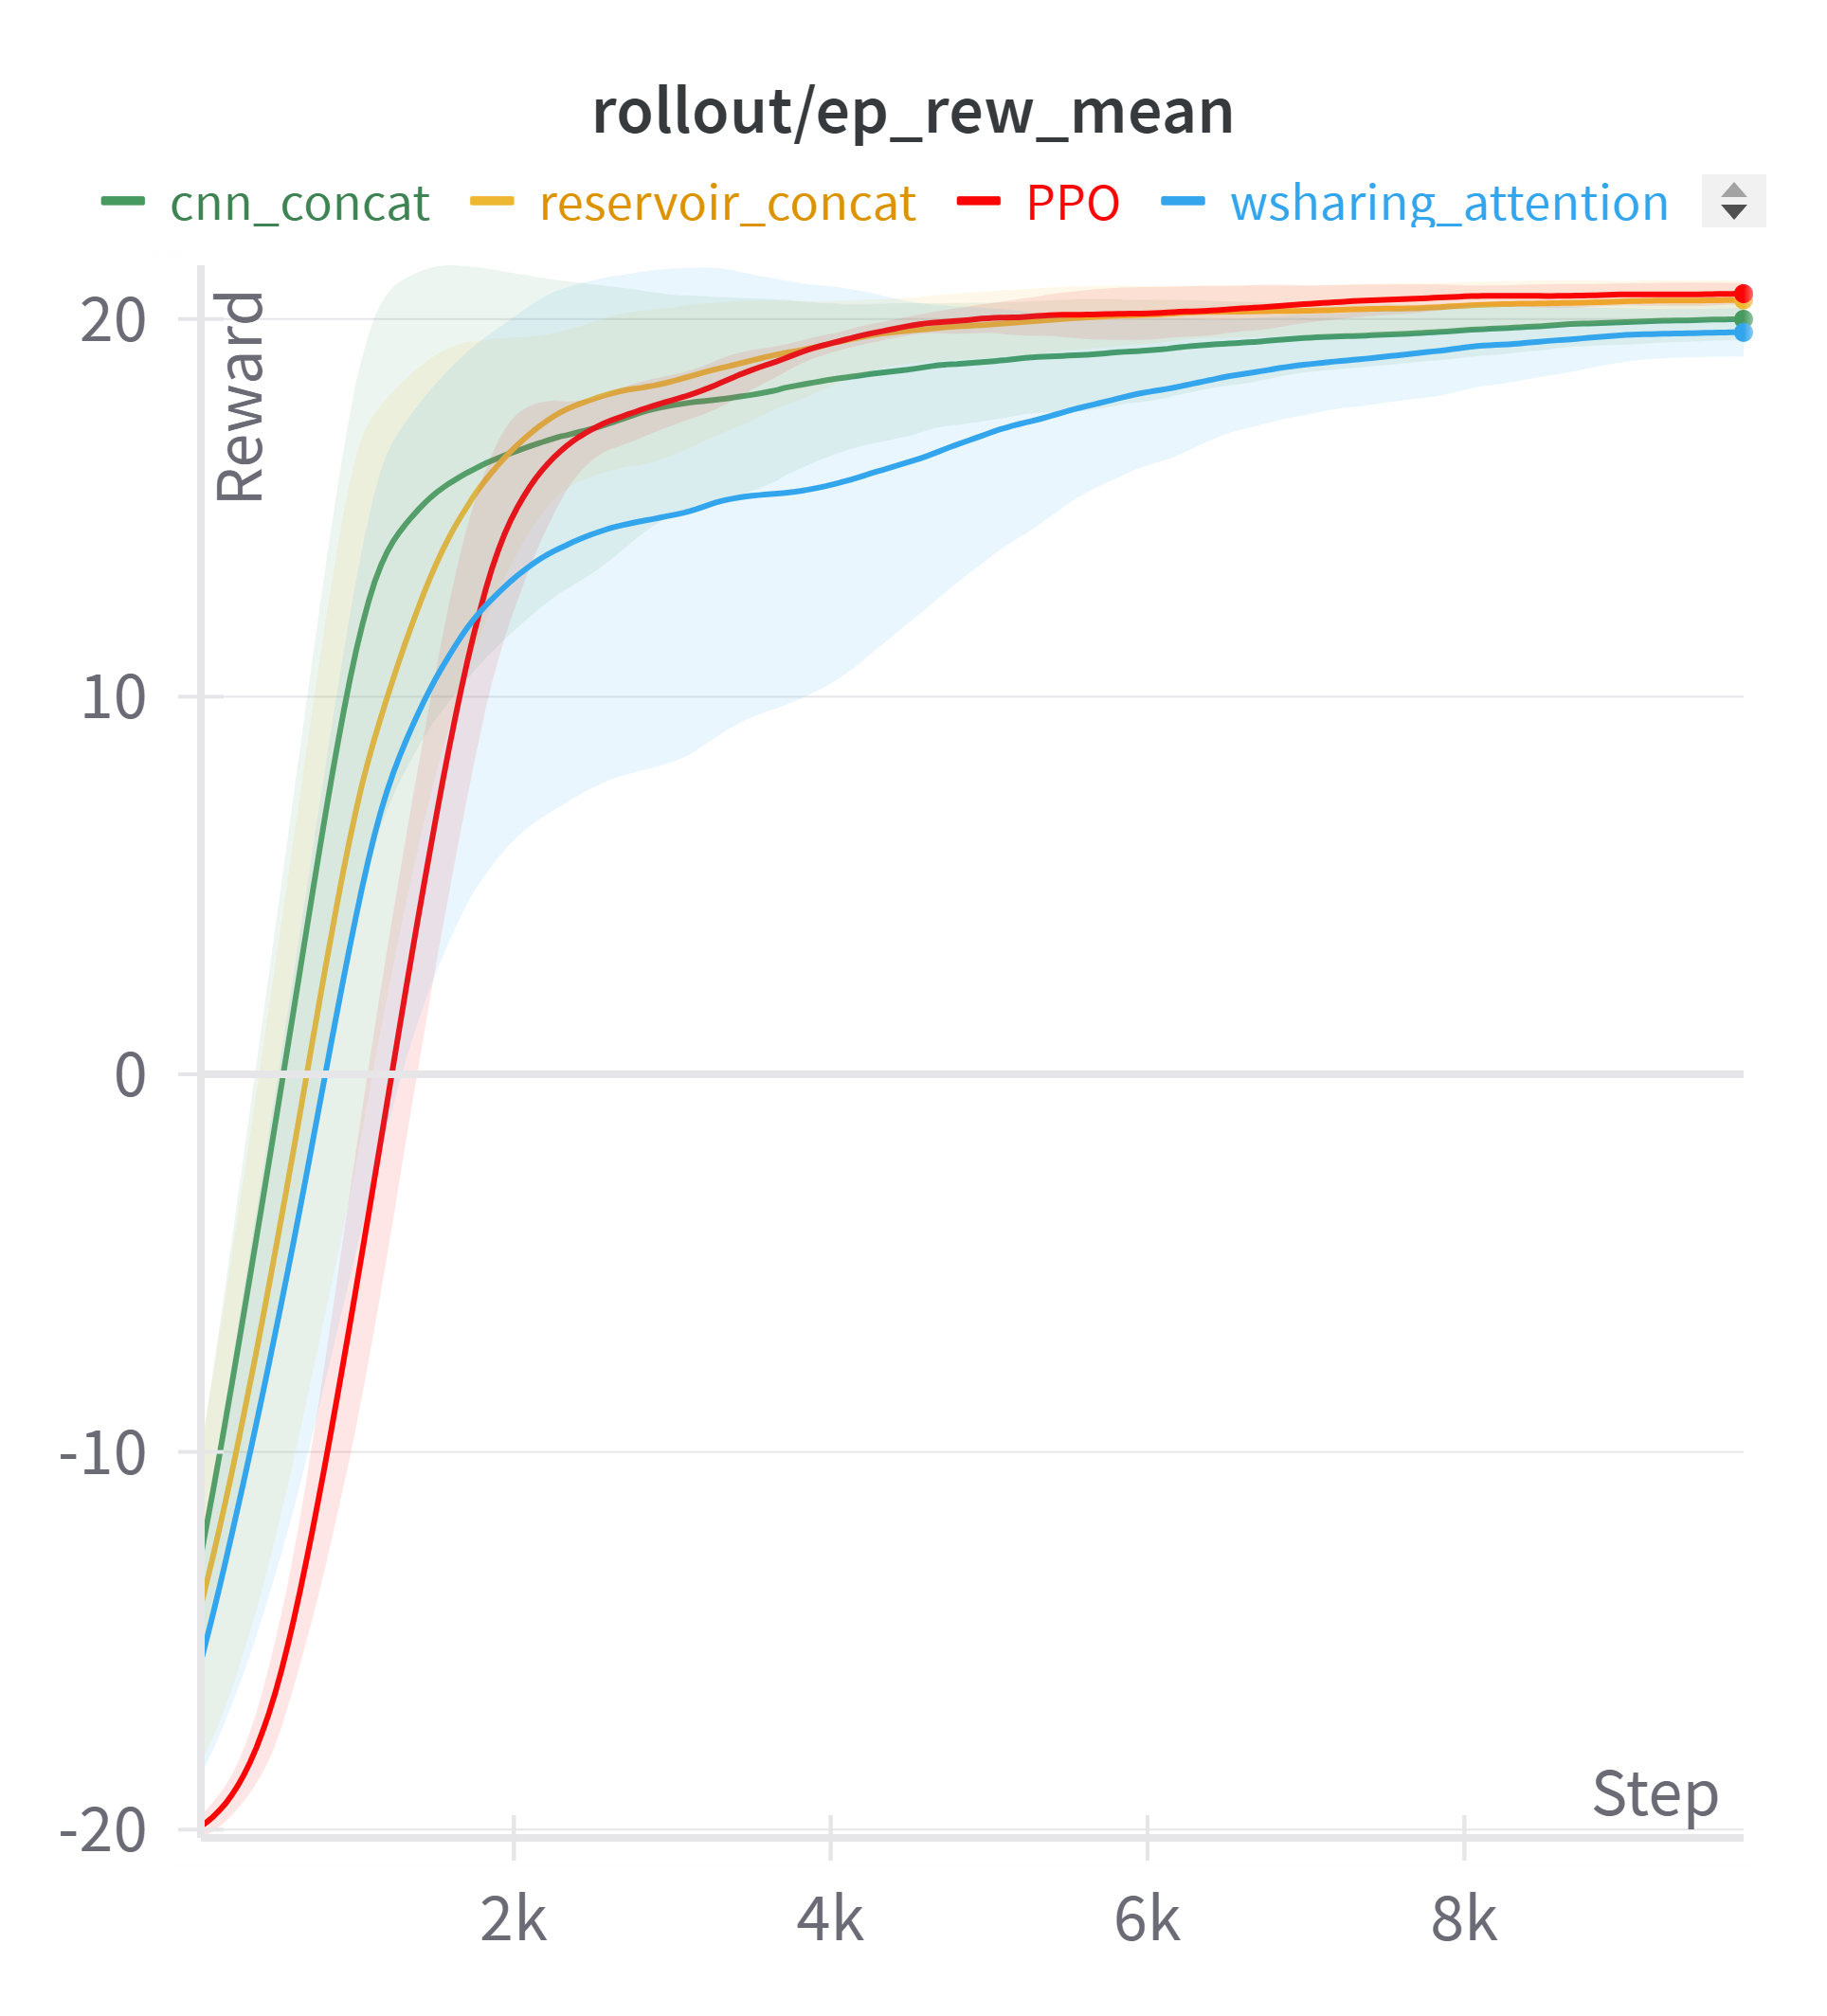
\includegraphics[width=\textwidth]{images/pong_train}
        \caption{\texttt{Pong}}
        \label{fig:pongtraining}
    \end{subfigure}
    \hfill
    \begin{subfigure}[b]{0.32\textwidth}
        \centering
        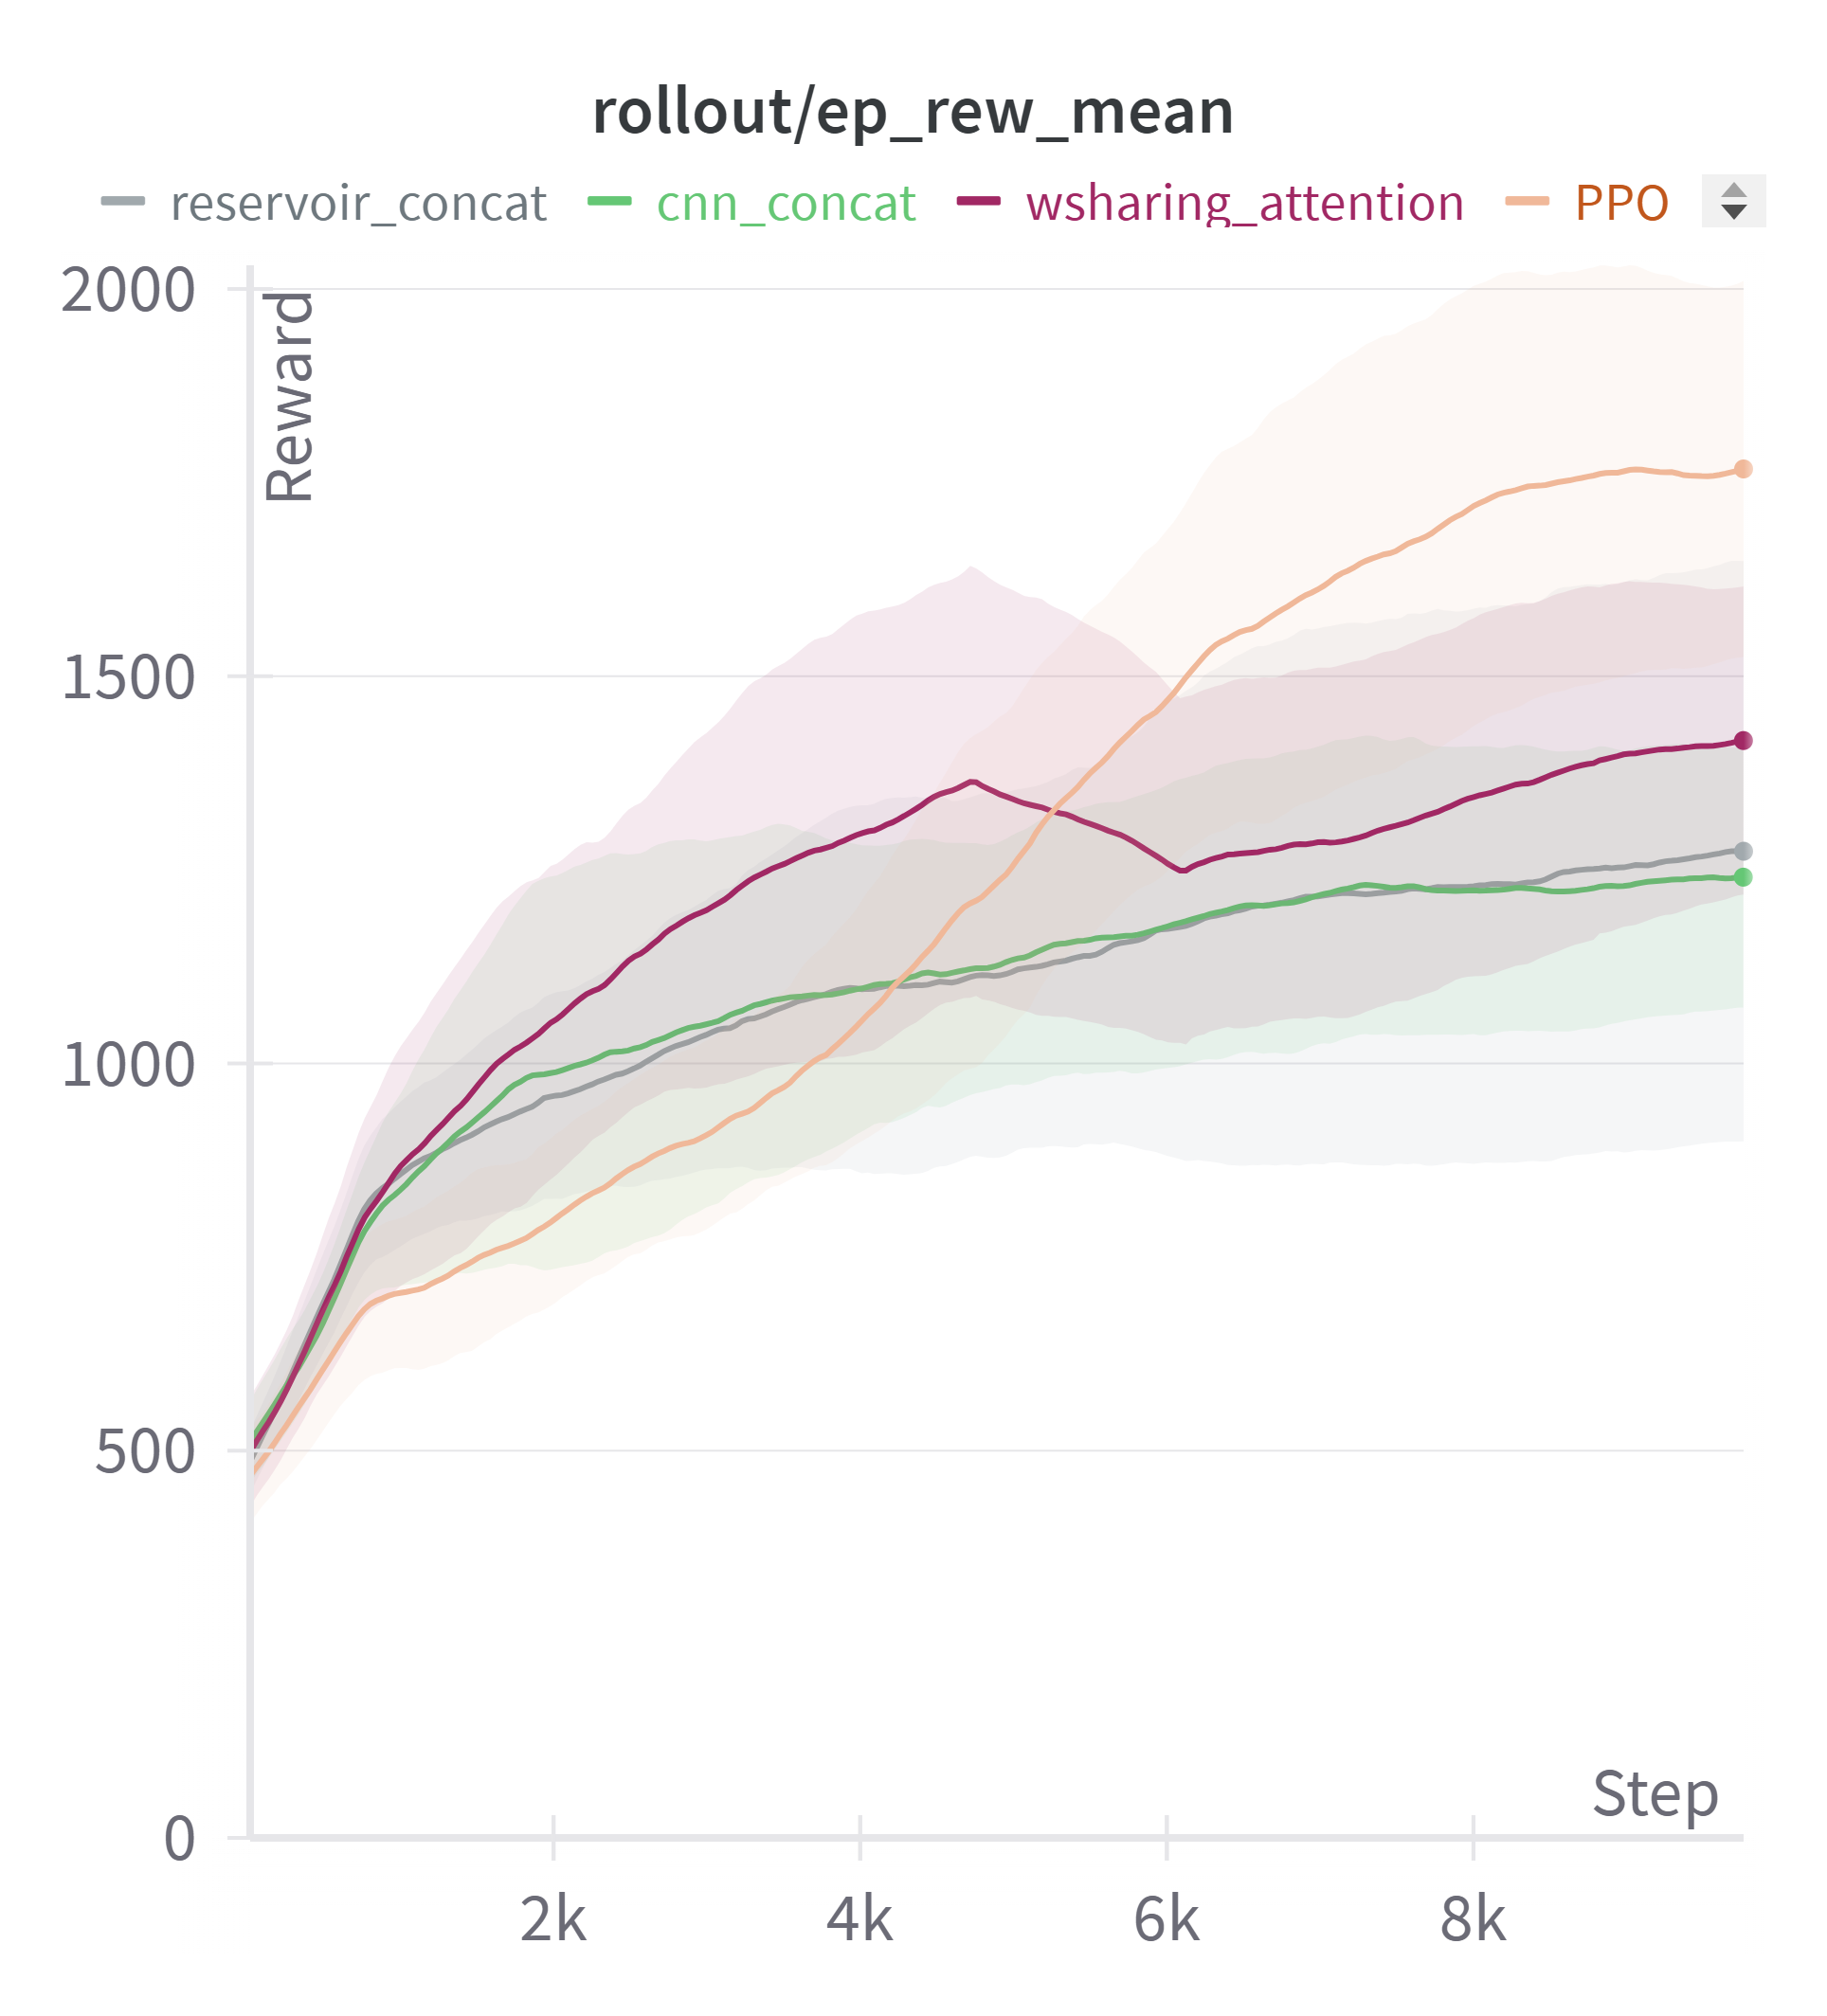
\includegraphics[width=\textwidth]{images/mspacman_train}
        \caption{\texttt{Ms.Pacman}}
        \label{fig:mspacmantrain}
    \end{subfigure}
    \hfill
    \begin{subfigure}[b]{0.32\textwidth}
        \centering
        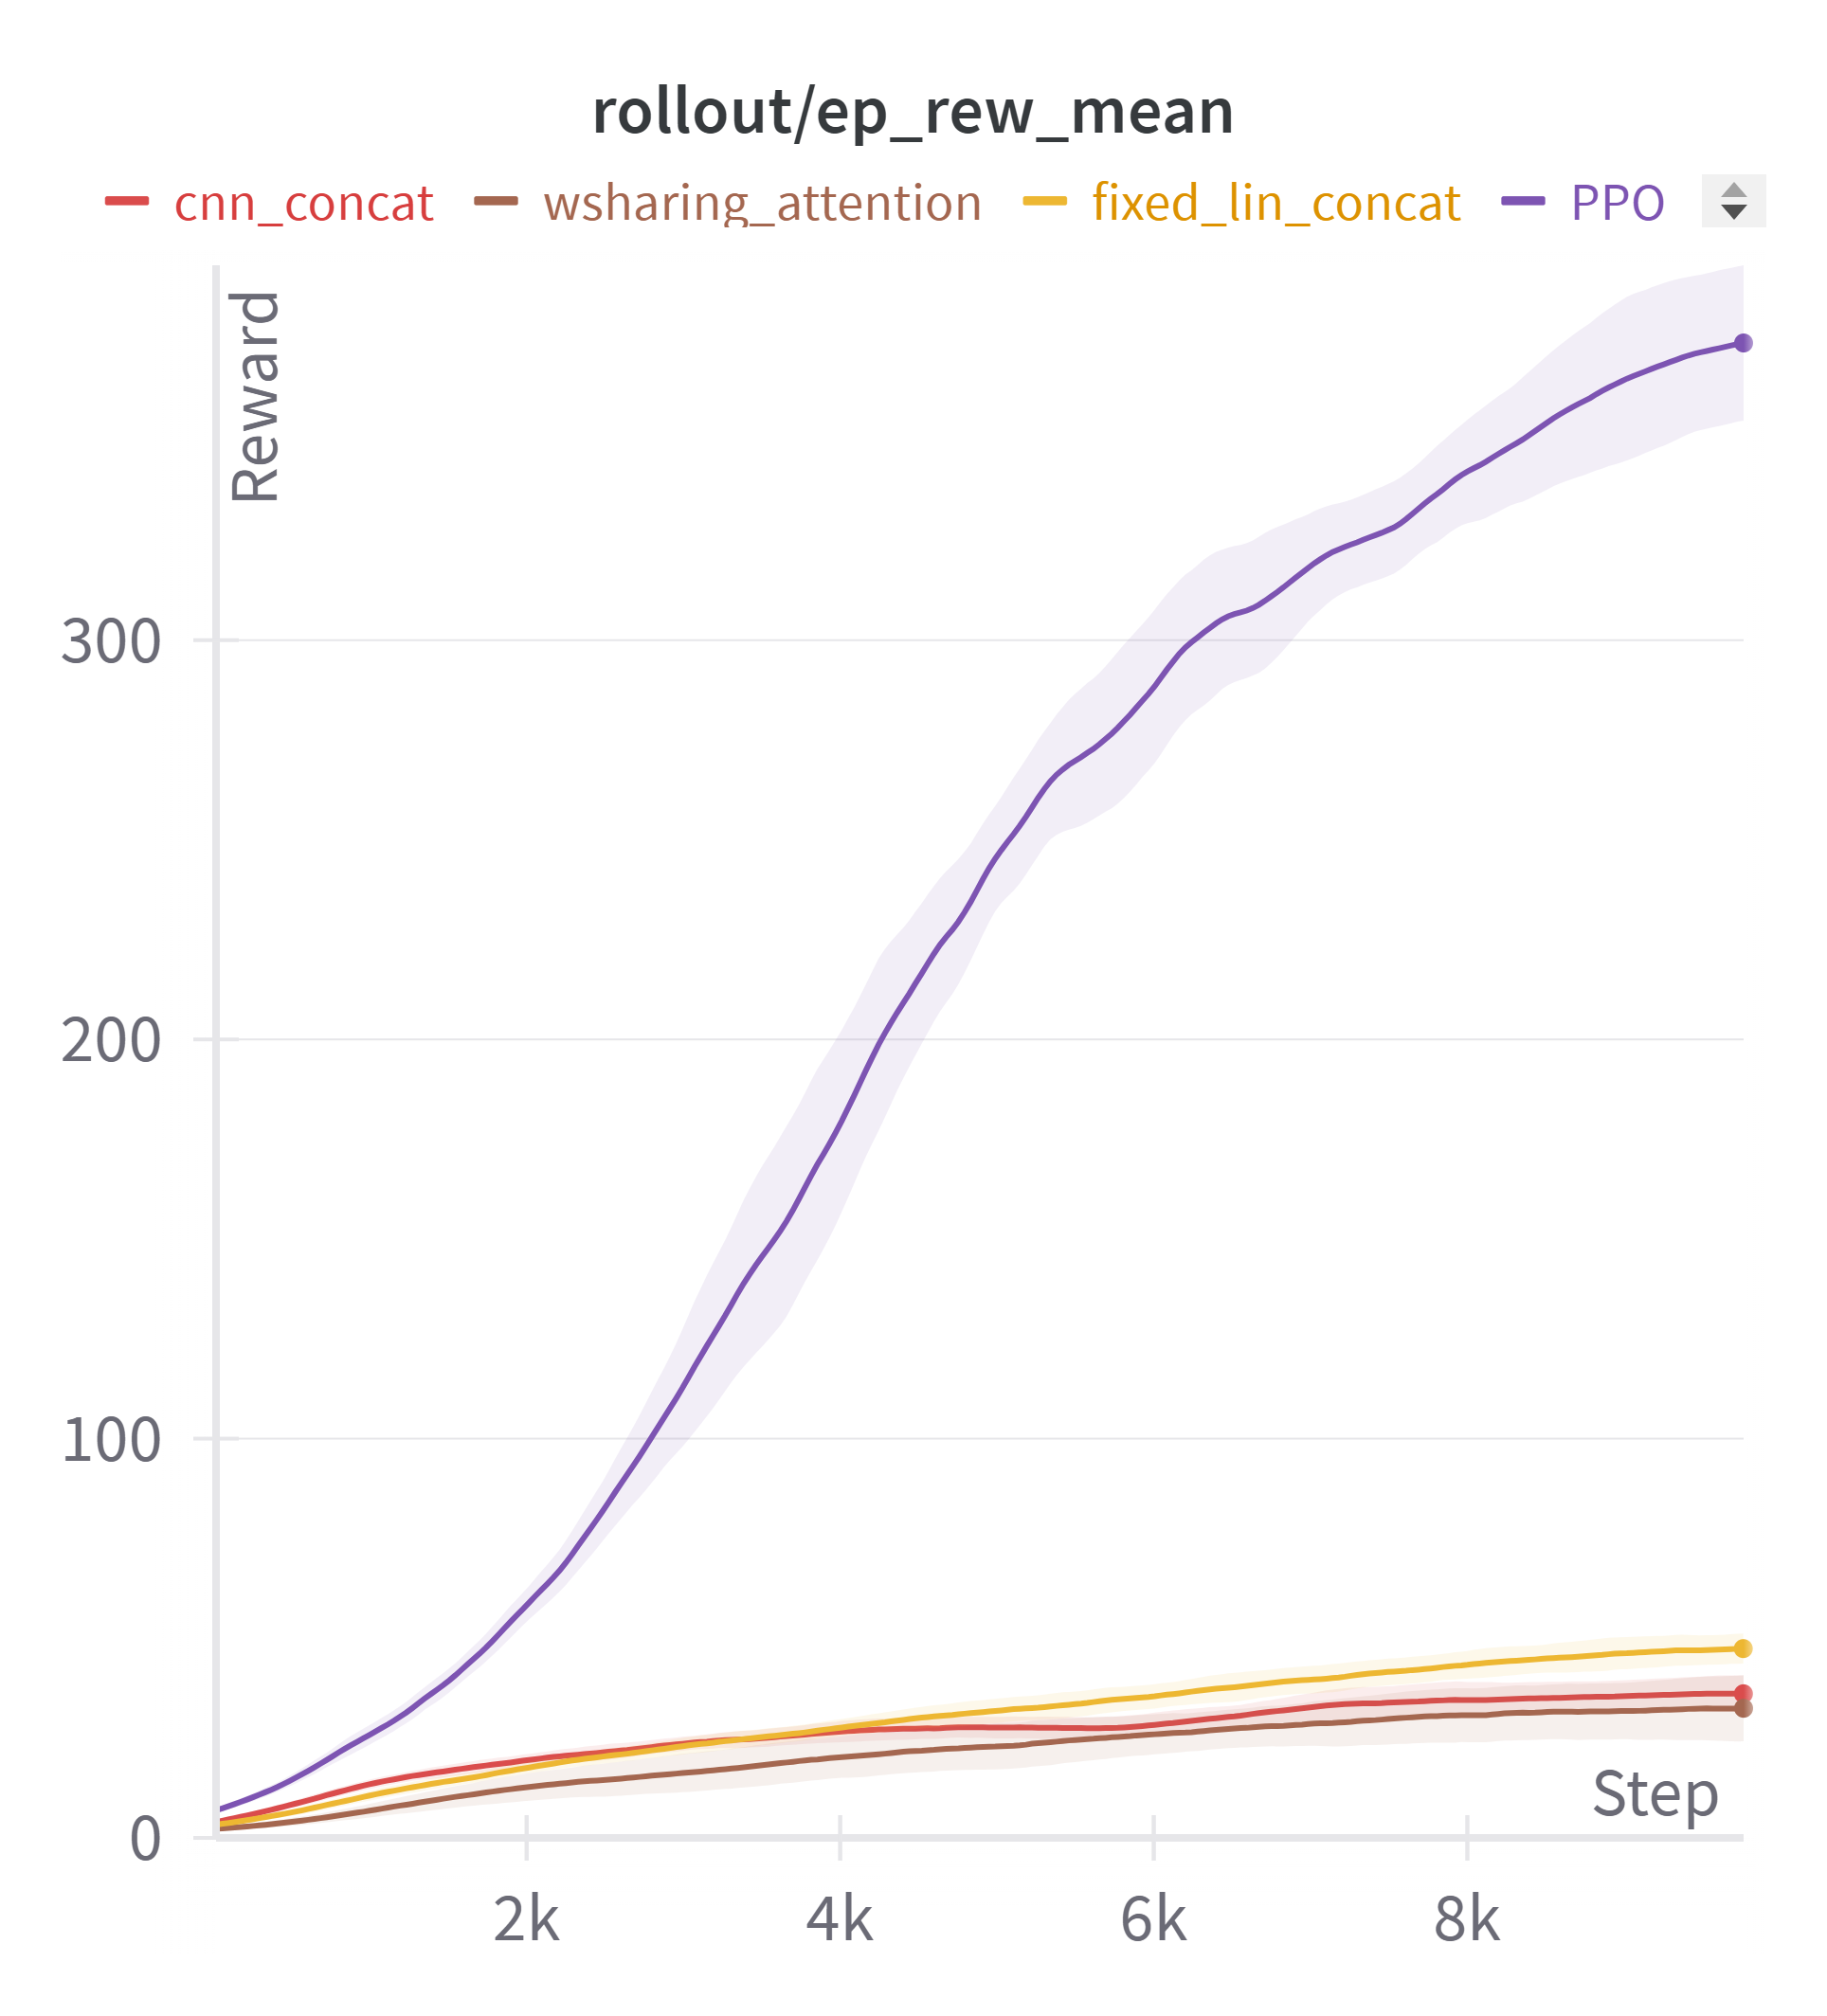
\includegraphics[width=\textwidth]{images/breakout_train}
        \caption{\texttt{Breakout}}
        \label{fig:breakouttrain}
    \end{subfigure}
    \caption{Cumulative reward of the best performing combination modules during training on different games. Each subfigure shows the mean score, with shaded areas indicating the standard deviations across multiple run of the same agent.}
    \label{fig:trainresults}
\end{figure}


To evaluate our agents, we selected for each agent the run that performed best during training, and we tested it across \texttt{5} random seeds for \texttt{50} episodes.
The seeds specifically are \texttt{47695}, \texttt{32558}, \texttt{94088}, \texttt{71782} and \texttt{66638}.
Table~\ref{tab:results} reports the averaged results during the evaluation of the best agent during training.

\begin{table}[ht]
\centering
    \begin{tabular}[b]{lll}
                \multicolumn{1}{l}{Environment}  &\multicolumn{1}{l}{\bf Agent} &\multicolumn{1}{l}{\bf Reward} \\
                \hline \\
                \multirow{4}{*}{\texttt{Pong}} & \textbf{CNN} & \textbf{21 $\pm$ 0.00} \\
                                      & RES & 20.85 $\pm$ 0.29 \\
                                      & \textbf{WSA} & \textbf{21 $\pm$ 0.00} \\
                                      & \textbf{PPO} & \textbf{21 $\pm$ 0.00}\\

                                      \hline \\
                \multirow{4}{*}{\texttt{Ms.Pacman}} & CNN & 1801.30 $\pm$ 20.95 \\
                                      & RES & 1369.27 $\pm$ 565.23 \\
                                      &\textbf{WSA} & \textbf{2530.20 $\pm$ 23.09} \\
                                      & \underline{PPO} & \underline{2258.40 $\pm$ 1.42}\\
                                      \hline \\

                \multirow{4}{*}{\texttt{Breakout}}
                                      & CNN & 65.98 $\pm$ 1.62 \\
                                      & FIX & 87.17 $\pm$ 6.87 \\
                                      & WSA & 99.58 $\pm$ 6.66 \\
                                      & \textbf{PPO} & \textbf{413.51 $\pm$ 1.10}\\
    \end{tabular}
    \caption{Performance during evaluation averaged across 5 different seeds.}
    \label{tab:results}
\end{table}


Analyzing these results, focusing on \textit{Pong} Fig.~\ref{fig:pongtraining} and \textit{Ms.Pacman} Fig.~\ref{fig:mspacmantrain},
we can see that our approach WSA and other combination modules yields a high reward in the first stages of the training process.
This suggests that FMs, as we hypothesized in the premises of our work, deliver valuable insights and a broad understanding of various elements in the environment without requiring additional training, as they offer an insightful and comprehensive base of knowledge straight out of the box.

In the case of \textit{Pong}, the performance of the agents is almost identical during training.
The agents reach the maximum reward of \texttt{21} in the first stages of training.
We notice that WSA in this case is a bit slower than the other agents to reach the maximum reward on average, but it is still able to reach it.
On the other hand, in \textit{Ms. Pacman}, the agents show a different behavior, showing a more marked difference in performance during training between WSA and other combination modules.
In the second phase of training, eventually, end-to-end PPO catches up and reaches a higher final reward score.
This suggests that the FMs' representations are more effective in the early stages of training, providing the agent with many insights about the environment and allowing it to learn faster.
The fact that end-to-end PPO reaches a higher final score may suggest that agents trained with FMs need to be refined to perform at their best.
Again, it is important to note that we did not perform any hyperparameter search, and the agents' performance could be further improved by tuning the hyperparameters.

Nevertheless, looking at the evaluation results in Table~\ref{tab:results}, WSA matches the maximum reward (\texttt{21}) on \textit{Pong} and achieves a higher score (\texttt{2530}) on \texttt{Ms. Pacman} than end-to-end PPO (\texttt{2258}).
From these results, we can make two important considerations.
The first one is the difference between training and evaluation scores.
In particular, in \textit{Ms. Pacman} is more marked, WSA provides a solid generalization for the task, scoring around \texttt{1250} during training compared to \texttt{2530} during evaluation.
The second one concerns the difference compared to PPO final score during learning.
With respect to end-to-end solutions, our approach has a limited number of components that are updated during training, in particular, the \textit{Fully-Connected Network} is only one layer.
This could lead to underfitting, and the performance of the agent could be further improved by increasing the complexity of the model.

We notice that the results of \textit{Breakout} are not as good as the other games.
These results will be discussed in the next section, where we will analyze the reasons behind this behavior and propose some possible solutions to improve the performance of the agent in this game.



\section{Breakout: Out of Distribution Data}\label{sec:breakout_study}
While on \textit{Pong} and \textit{Ms. Pacman} the agents performed well, reaching the maximum reward during training and achieving high scores during evaluation, the results on \textit{Breakout} were not as good.
WSA and the other combination modules did not work right out of the box, and the agents struggled to learn the environment.
Specifically, both in Figure~\ref{fig:breakouttrain} and in Table~\ref{tab:results}, the performance of WSA is extremely low compared to an end-to-end PPO (\texttt{99} vs \texttt{413}).
So, in this Section, we will analyze the possible reasons for the behavior of the agents in this environment.

As we analyzed in Section~\ref{sec:top-3-performer}, agents could suffer from underfitting problems due to the limited complexity of the model.
So, a first attempt to overcome the problem was to increase the number of parameters of the model, adding more expressive power to the network that learns the policy.
We believe that the \textit{Fully-Connected Network} may be too simple to capture the complexity of the environment, and the agents could benefit from a bigger network.
We increased the size of the policy learning network to three linear layers of size \texttt{1024}, \texttt{512}, and \texttt{256} respectively for the first, second, and third layer, and use ReLU as activation function to avoid vanishing gradients and allow the network to learn more complex patterns.
Figures~\ref{fig:breakout_policy},~\ref{fig:breakout_cnn_policy}, and~\ref{fig:breakout_fix_policy}
shows the learning curve of the agents during training.
Evaluation results are reported in Table~\ref{tab:breakout_results} where we refer to these experiments as \textit{Policy}.
With respect to the default scenario, there is an improvement in performance for all the agents, and in particular, WSA almost doubles its score, meaning that a more complex policy network can help the agent to learn the environment better, and can capture more information from the FMs' representations.
But the agents' performance is still far from the end-to-end PPO, WSA scored \texttt{156} compared to \texttt{413} of PPO\@.
We believe that the problem is not only due to the complexity of the model.



A second attempt to improve the performance of our agents was to better analyze the characteristics of the environments.
Considering \textit{Pong} and \textit{Ms. Pacman}, the screen remains relatively stable as the game progresses.
In \textit{Pong} the only moving objects are the ball and the paddles, while in \textit{Ms. Pacman} the ghosts move in the maze but the only disappearing objects are the dots.
In \textit{Breakout} instead, the environment dynamically evolves over time as more blocks are removed with score progression.
Leading to scenarios where the agent has to deal with fewer blocks and more open space.
While on the first stage of the game, the agent can earn points just by intercepting and bouncing the ball back, in the late stages the agent has to be more precise and hit the ball in the right direction to break the remaining blocks.
This poses a \textbf{distributional shift} problem between training and test data.
Our initial training data, collected from random agents, lacks late-game scenarios with few blocks remaining.
This could lead to situations where the FMs are not able to generalize well to unseen data and produce representations that are not informative enough for the agent.
For example, FMs like \textit{OKK} could output the wrong position of the ball or the blocks, and this could lead to a wrong decision by the agent.


To address the problem and show the consequences of a limited training dataset, we trained an end-to-end PPO agent, and we used it to collect new data from both random and expert agents to cover early and late game scenarios.
Then, we retrain all the FMs and RL agents using a single layer \textit{Fully-Connected Network} of \texttt{256} units as before.
Significant improvements are observed, as shown in Figure~\ref{fig:breakout_expert} for WSA and Table~\ref{tab:breakout_results}, where we refer to these experiments as \textit{Mixed}.
Notably, WSA demonstrates a substantial increase in the agent's final score going from \texttt{156} to \texttt{345}, approaching the performance of PPO\@.
Also, FIX shows a significant improvement in evaluation score, going from \texttt{87} to \texttt{199}.
This suggests that the agent's performance is highly dependent on the quality of the training data, and the agent can perform at most as well as the FMs do.
The better the FMs are, the better the agent will perform.
Even though the FMs are trained with mixed data, there may be some scenarios where they are not able to provide the right information, and the agent could benefit from ignoring them.
Unlikely, as we can see in Figures~\ref{fig:breakout_cnn_mixed} and~\ref{fig:breakout_fix_mixed}, the other combination modules do not show the same improvement in training, and the agents' performance is still lower than WSA\@.
This may be due to the fact that WSA can weight the contribution of each pre-trained model, such that can ignore the less informative ones.
The other combination modules do not have this capability, and they are forced to use all the pre-trained models, even the less informative ones.


To complete the set of experiments, we also tested the combination of the two previous configurations.
We increased \textit{Fully-Connected Network} and we used mixed datasets.
Figures~\ref{fig:breakout_expert_policy},~\ref{fig:breakout_cnn_expert_policy},~\ref{fig:breakout_fix_expert_policy} and Table~\ref{tab:breakout_results} shows the results of these experiments, where we refer to these experiments as \textit{Policy \& Mixed}.
We notice how the combination of the two strategies yields the best-performing configuration of WSA with a slightly lower but competitive score to PPO (\texttt{387} vs \texttt{413}).


\begin{figure}[ht]
    \centering
    \begin{subfigure}[b]{0.32\textwidth}
        \centering
        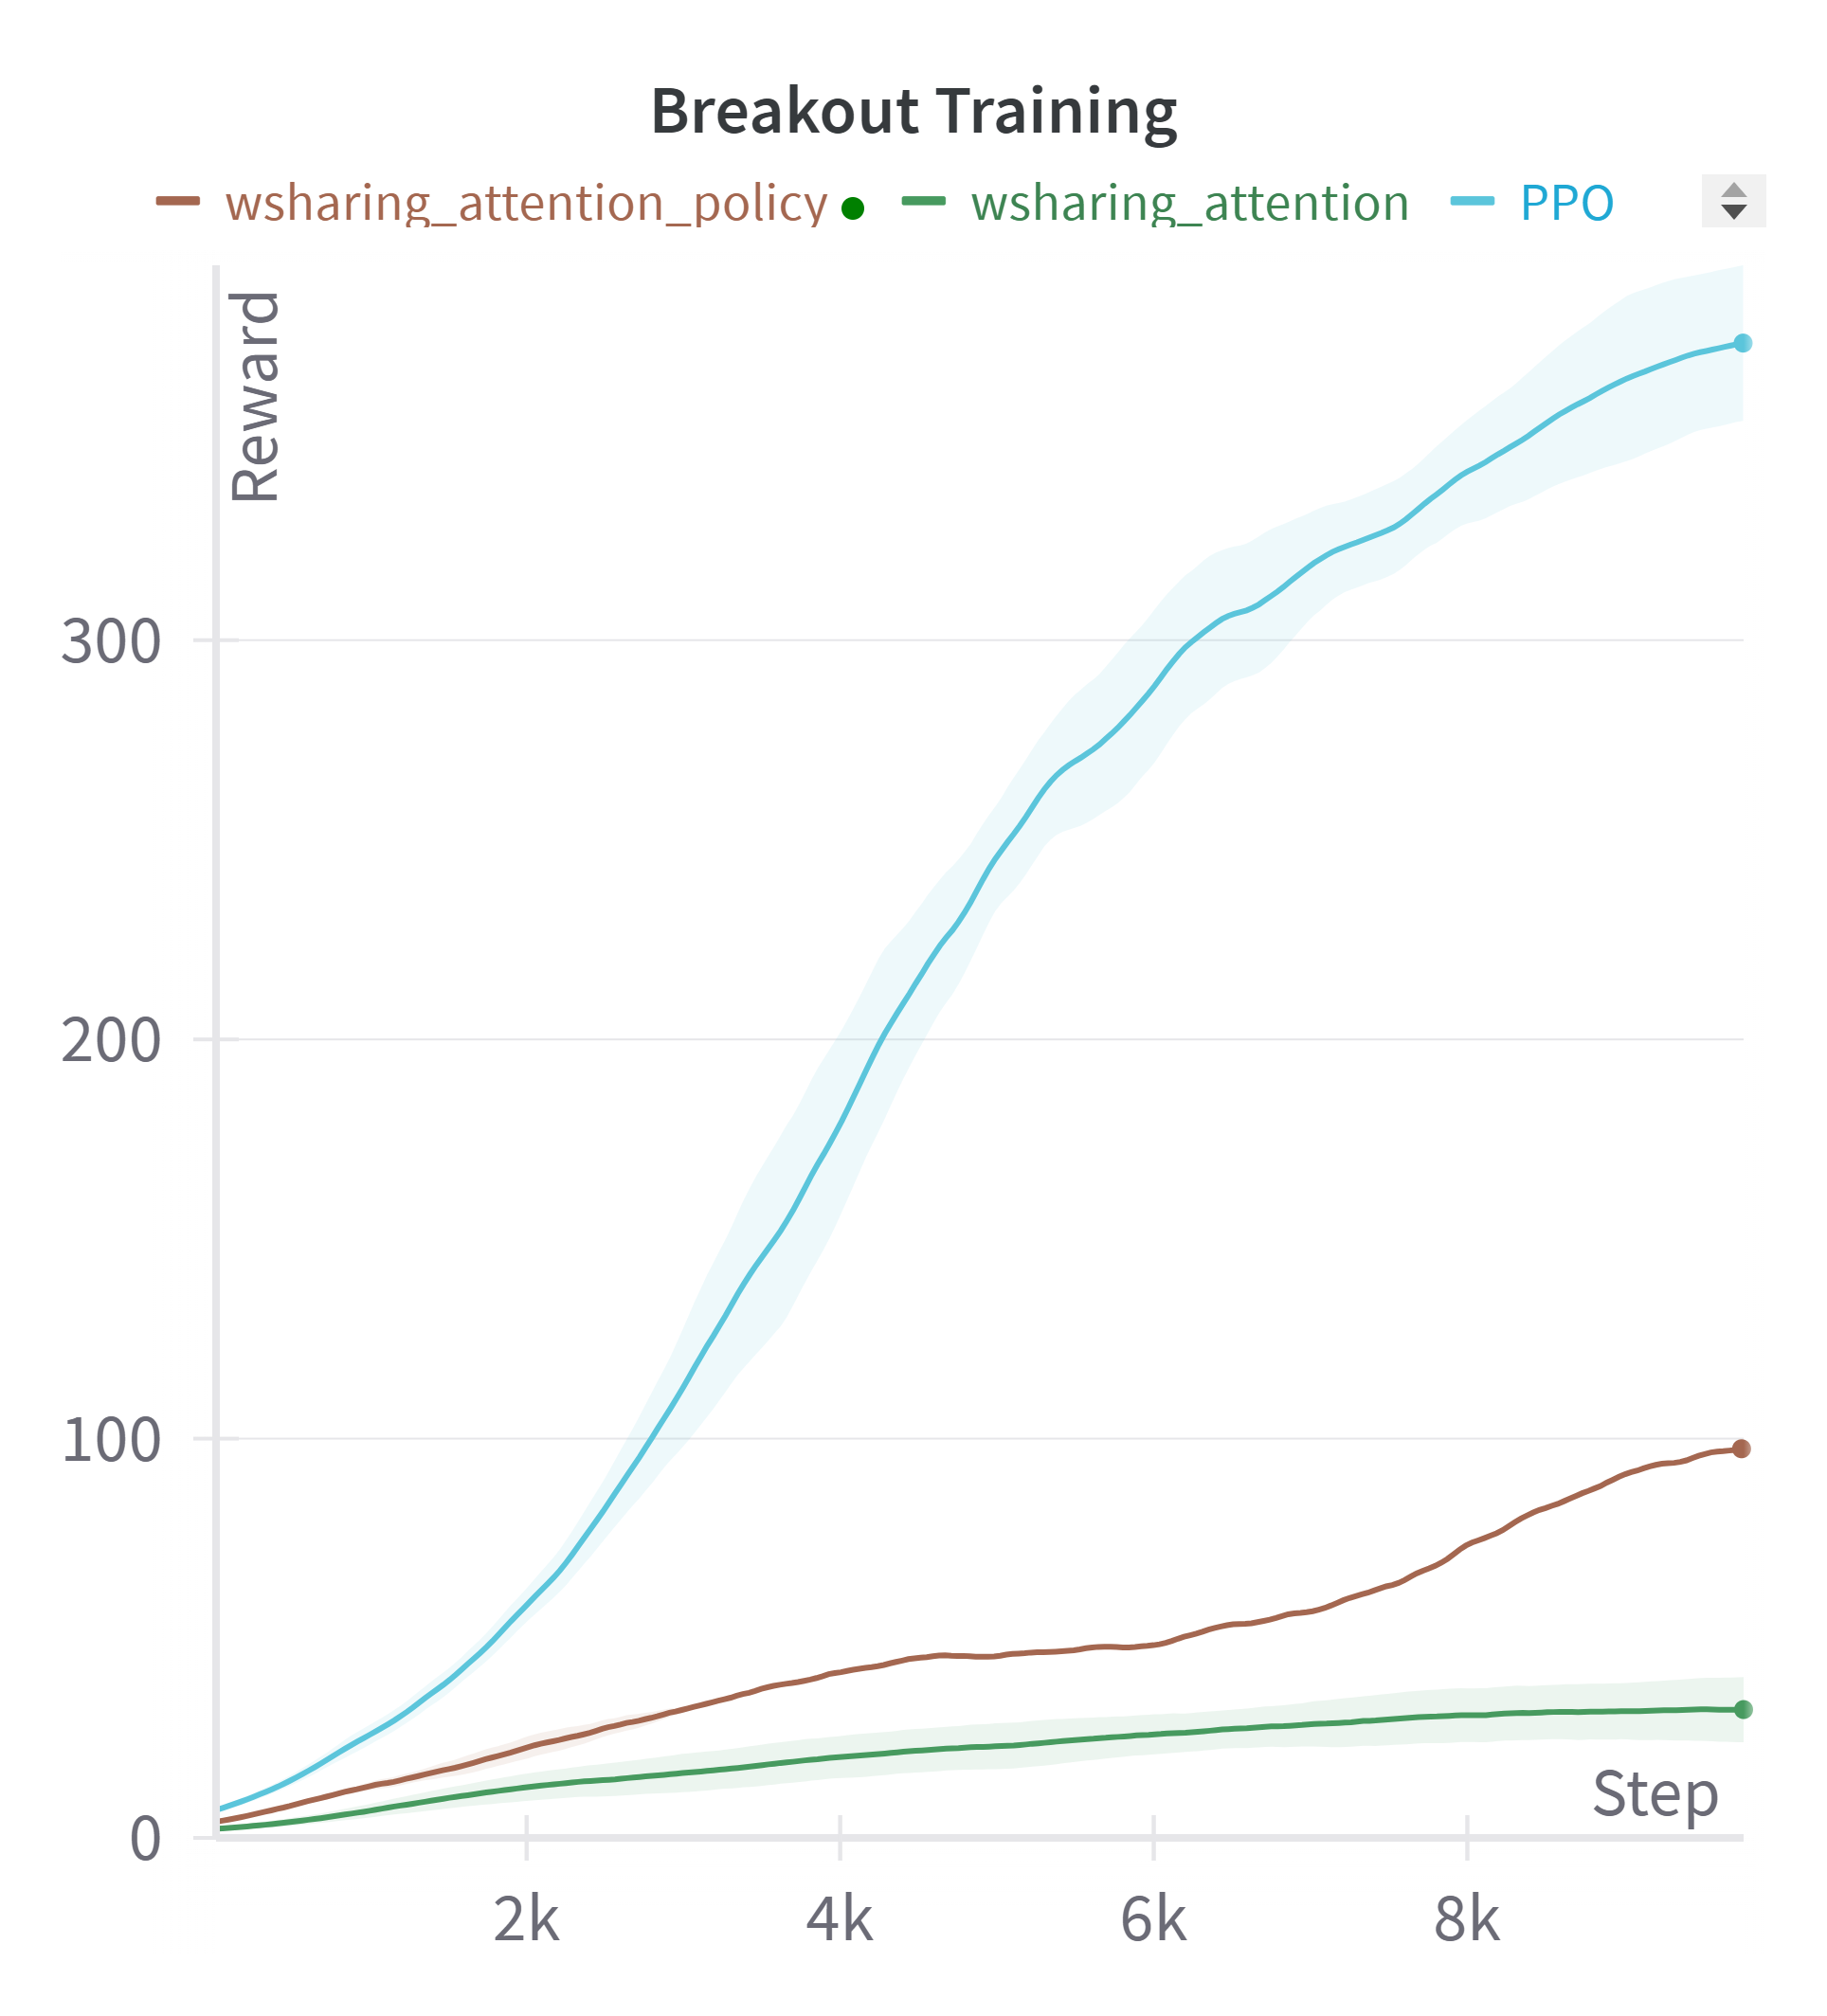
\includegraphics[width=\textwidth]{images/breakout_policy}
        \caption{Increasing MLP size}
        \label{fig:breakout_policy}
    \end{subfigure}
    \hfill
    \begin{subfigure}[b]{0.32\textwidth}
        \centering
        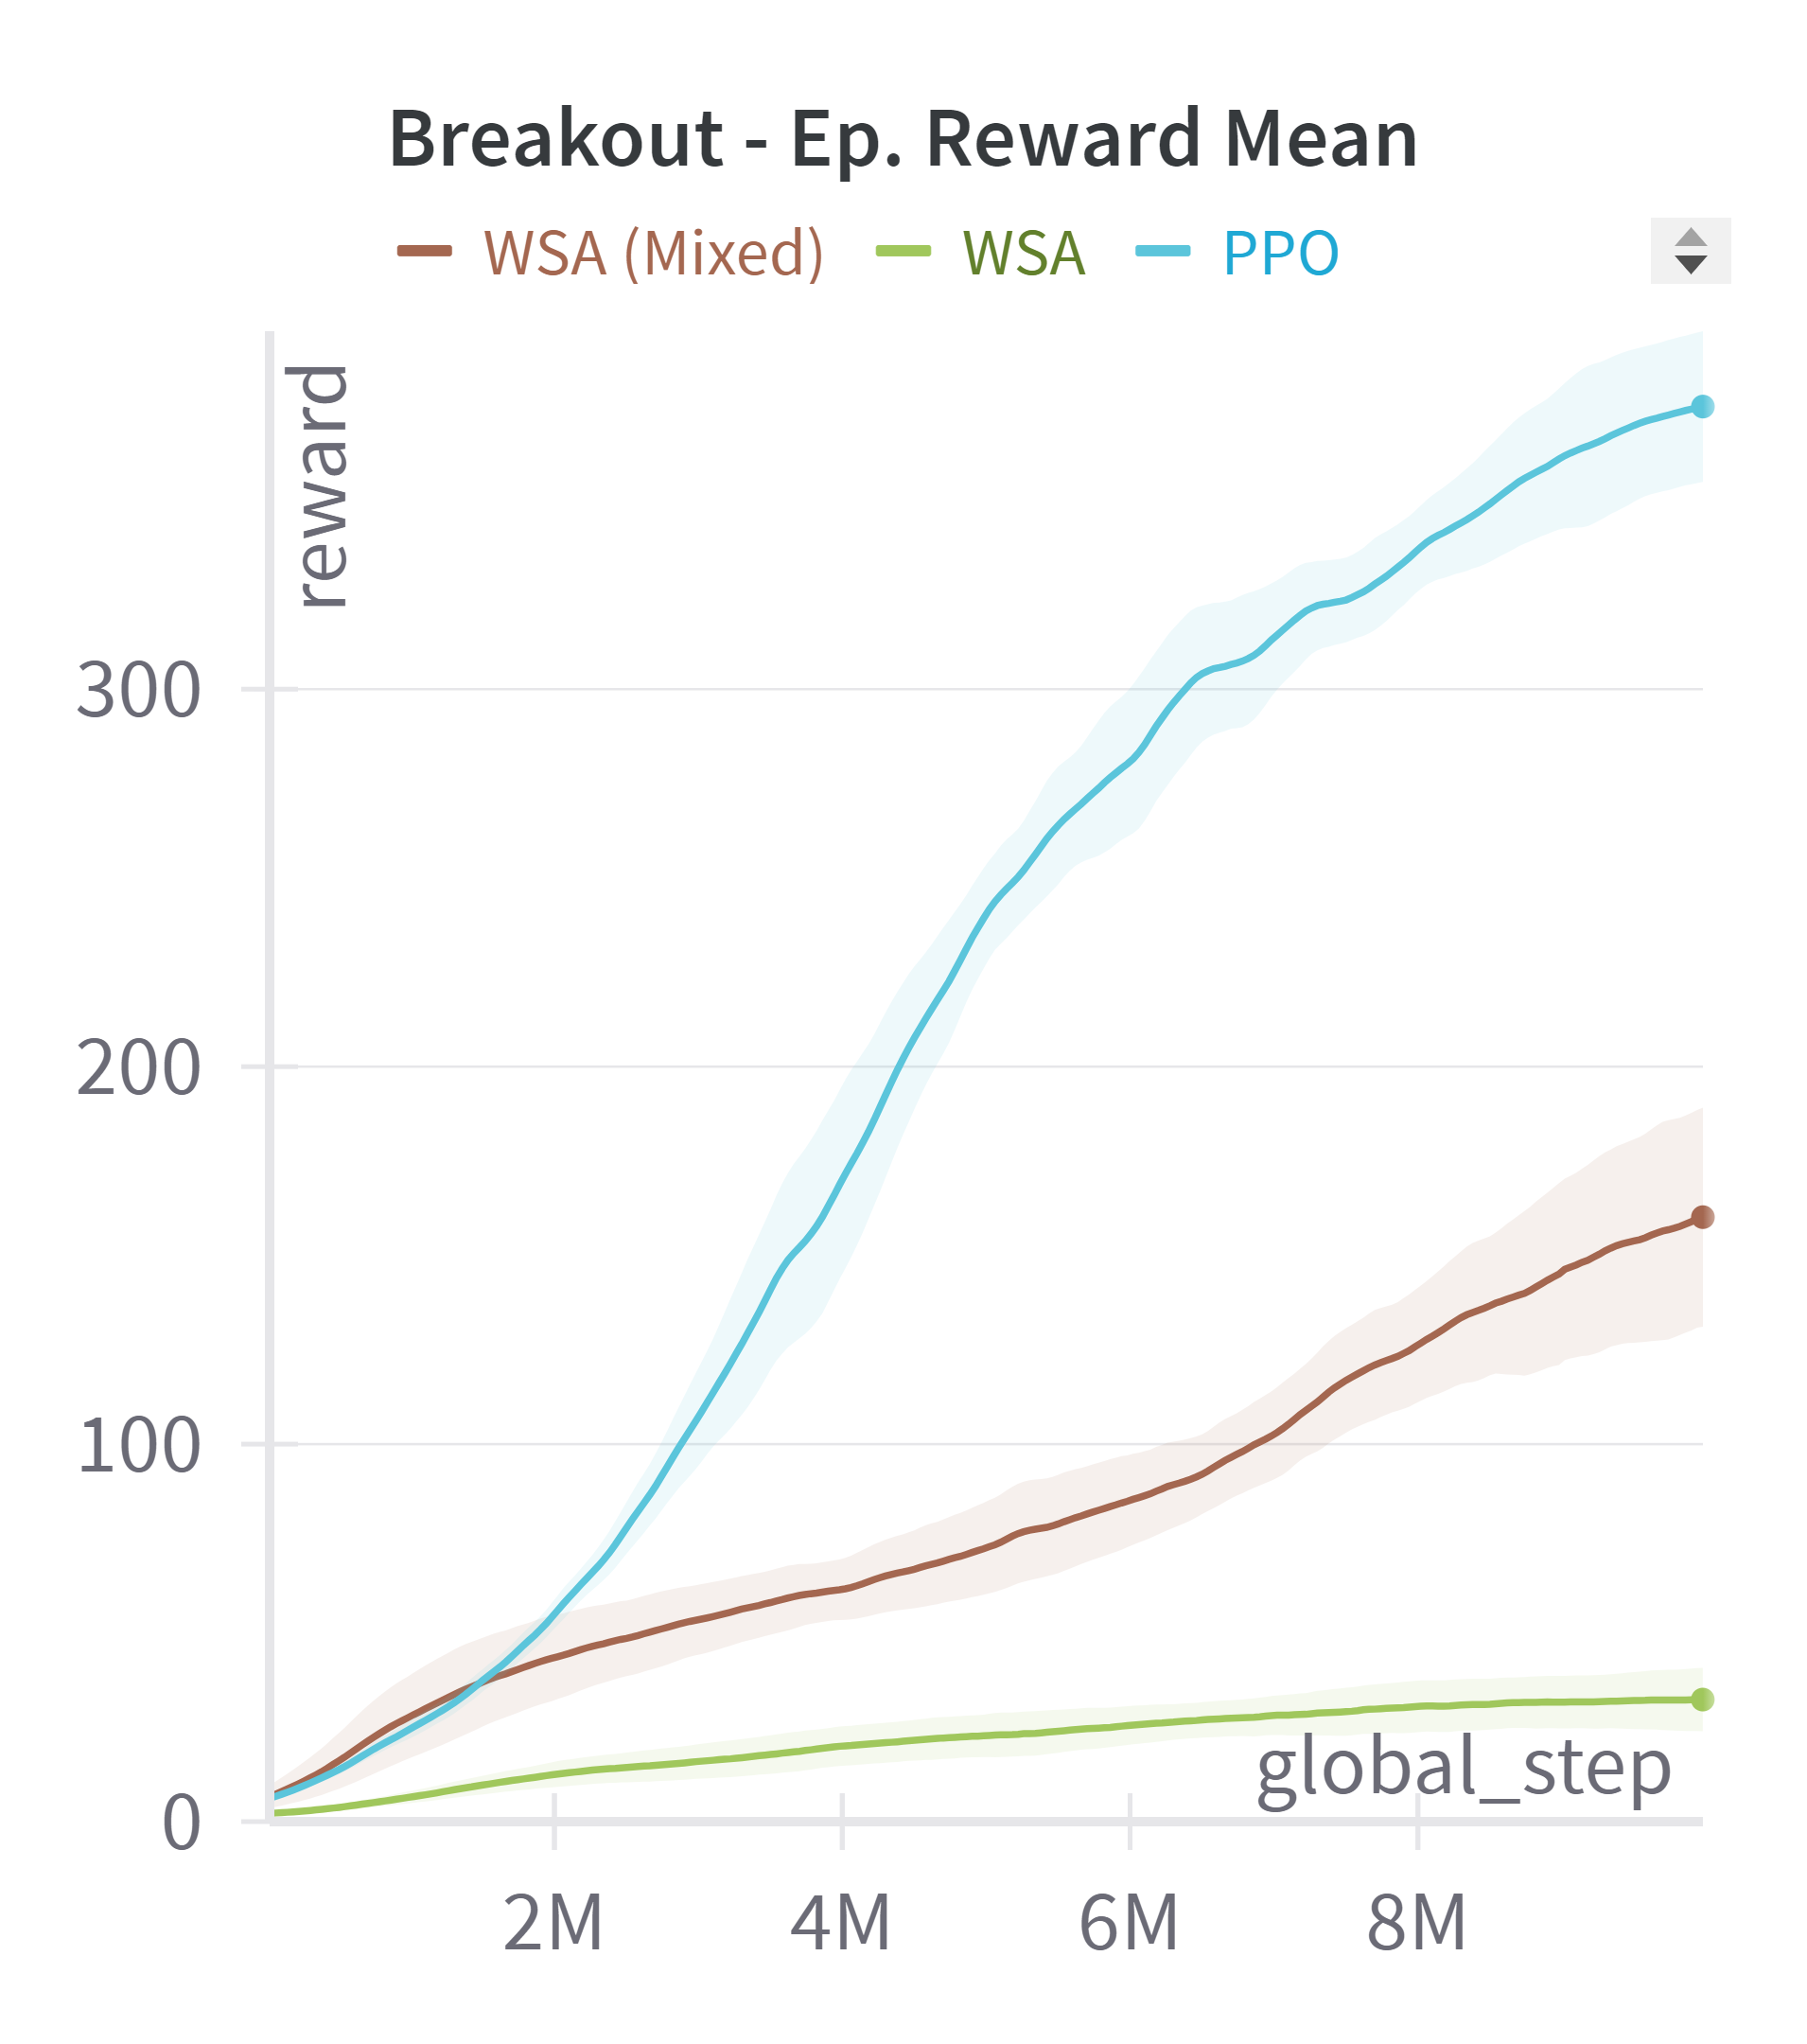
\includegraphics[width=\textwidth]{images/breakout_expert}
        \caption{Using Mixed Data}
        \label{fig:breakout_expert}
    \end{subfigure}
    \hfill
    \begin{subfigure}[b]{0.32\textwidth}
        \centering
        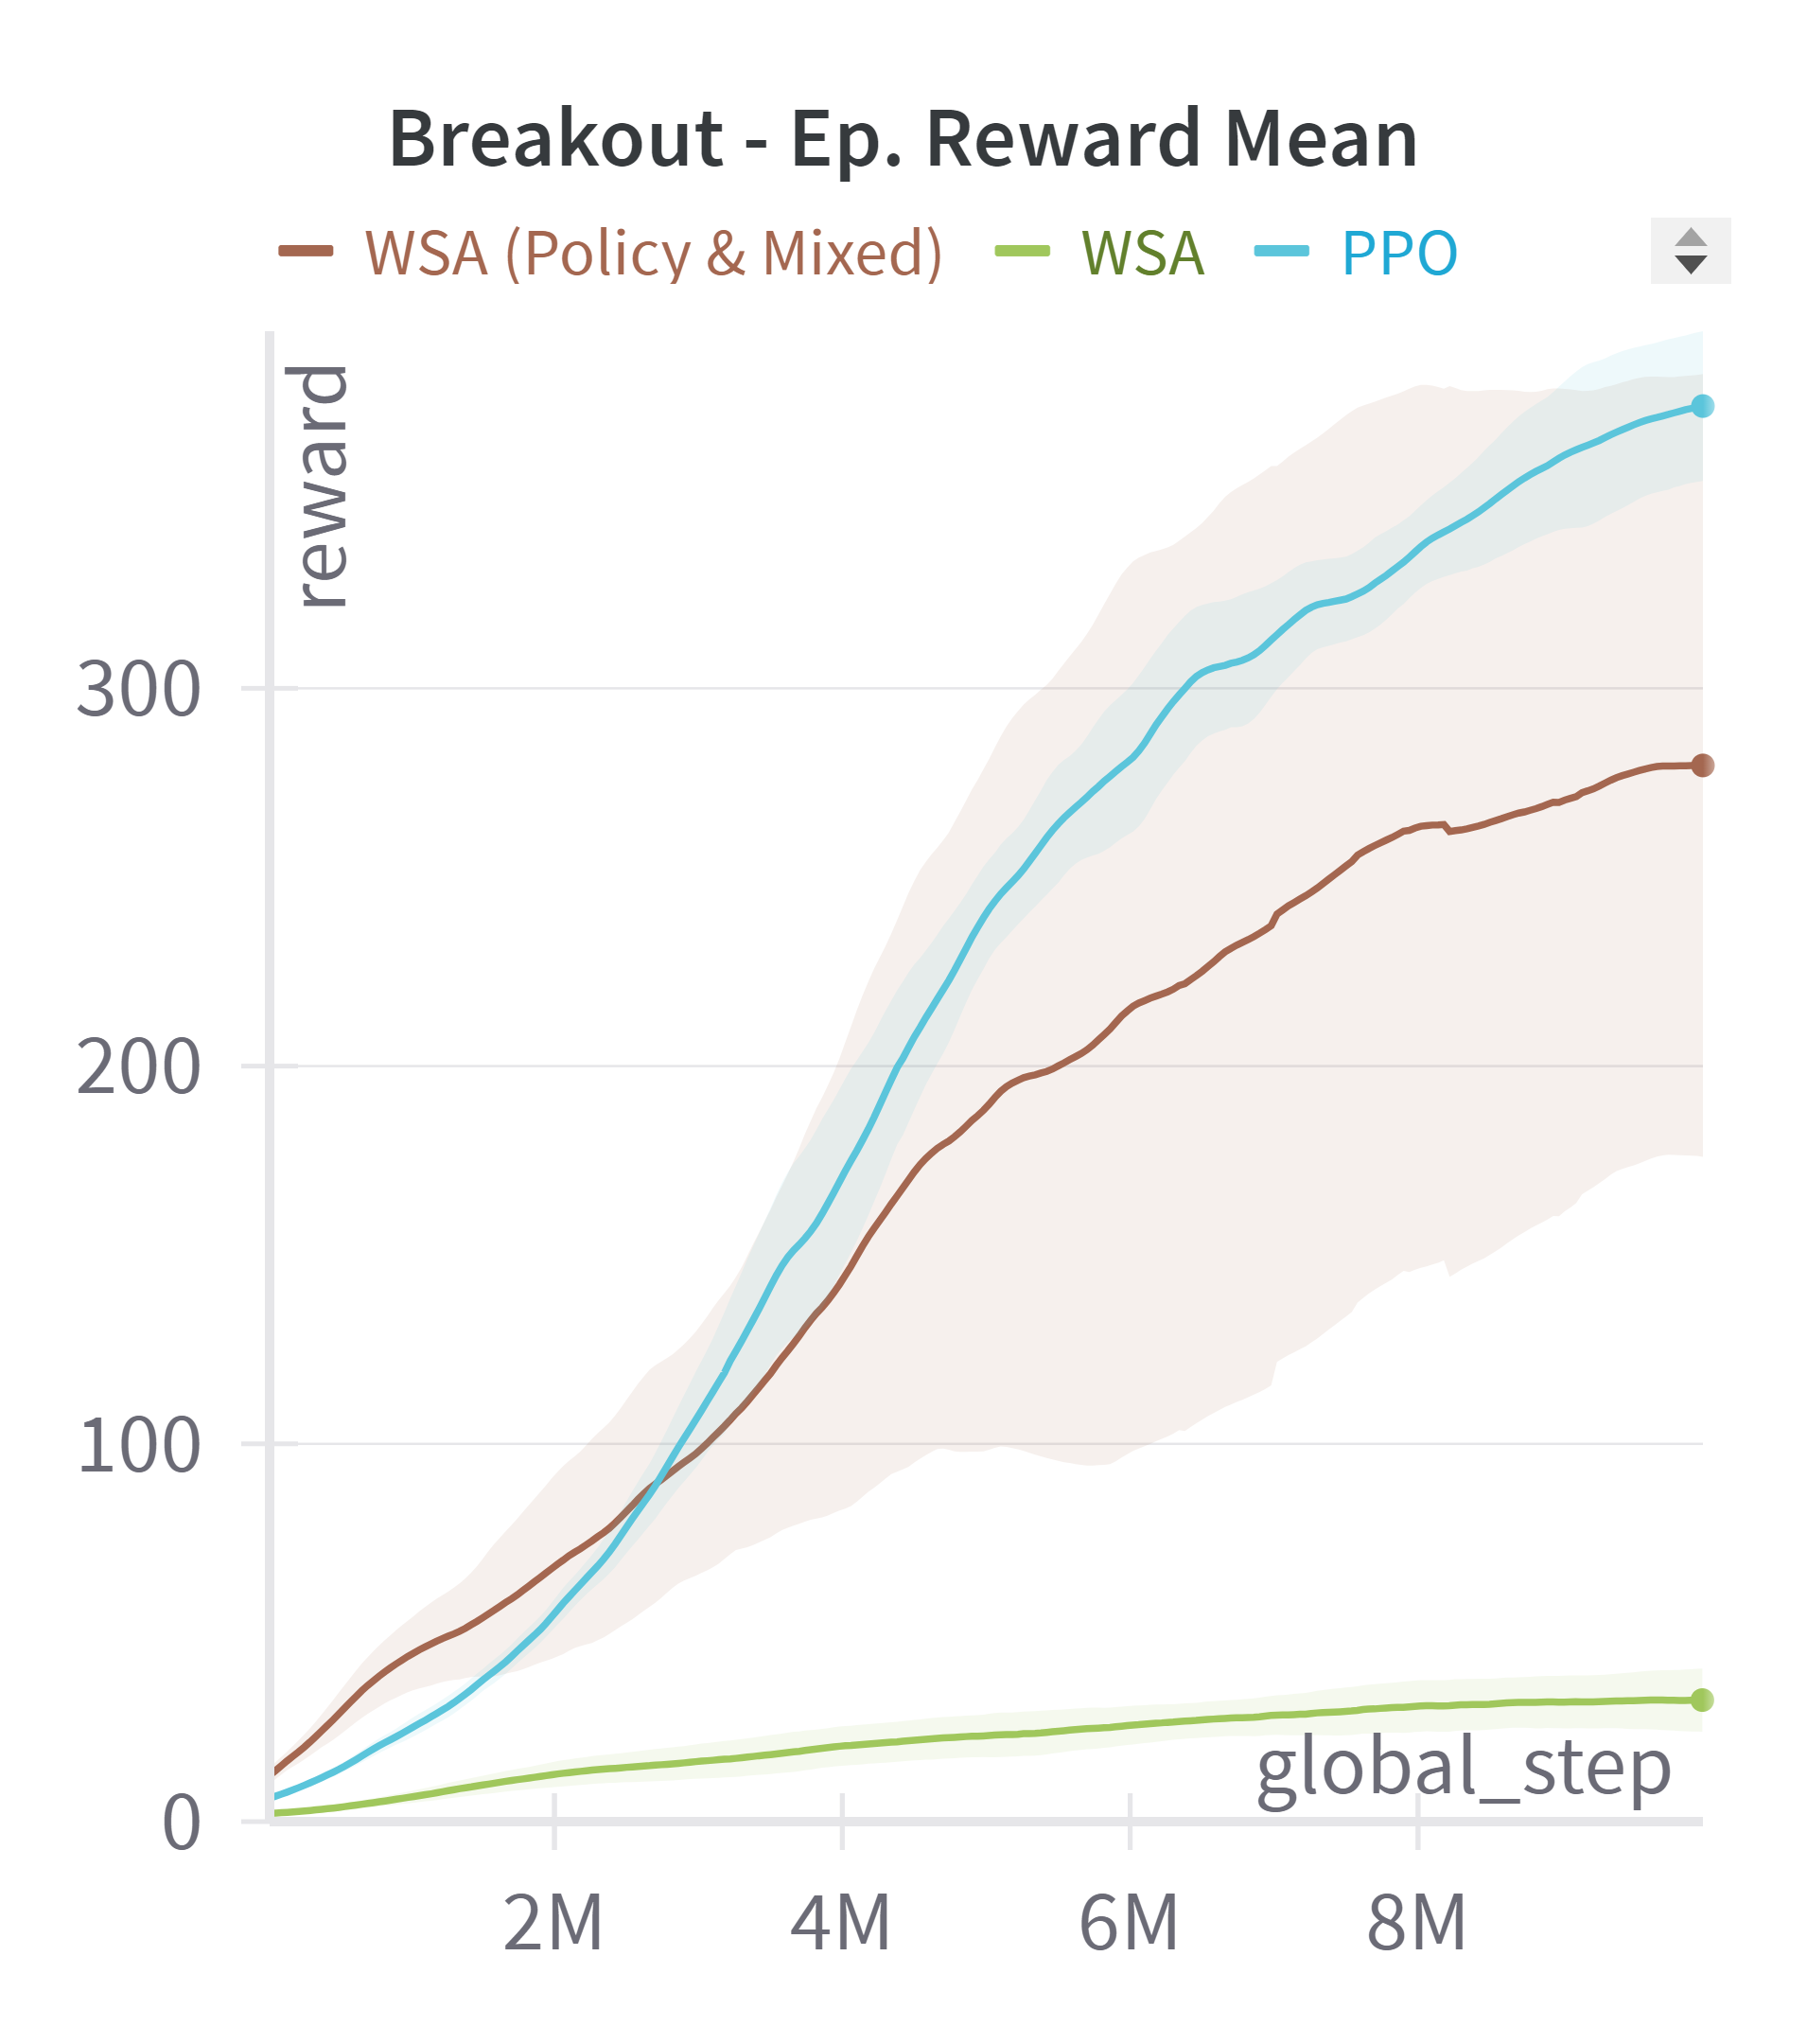
\includegraphics[width=\textwidth]{images/breakout_policy_mixed}
        \caption{Mixed Data + Increased MLP}
        \label{fig:breakout_expert_policy}
    \end{subfigure}~\caption{Performance comparison of WSA with PPO across various strategies on \textit{Breakout}. Each subfigure displays the average score with the standard deviation shaded. They report the different experiments to improve the performance of WSA: (\ref{fig:breakout_policy}) increasing the size of the \textit{Fully-Connected Network} on performance, (\ref{fig:breakout_expert}) pre-training the models using random data and expert data, and (\ref{fig:breakout_expert_policy}) combining the effect of increased \texttt{Fully-Connected Network} and expert data during pre-training.}
    \label{fig:breakout_study}
\end{figure}




\begin{figure}[ht]
    \centering
    \begin{subfigure}[b]{0.32\textwidth}
        \centering
        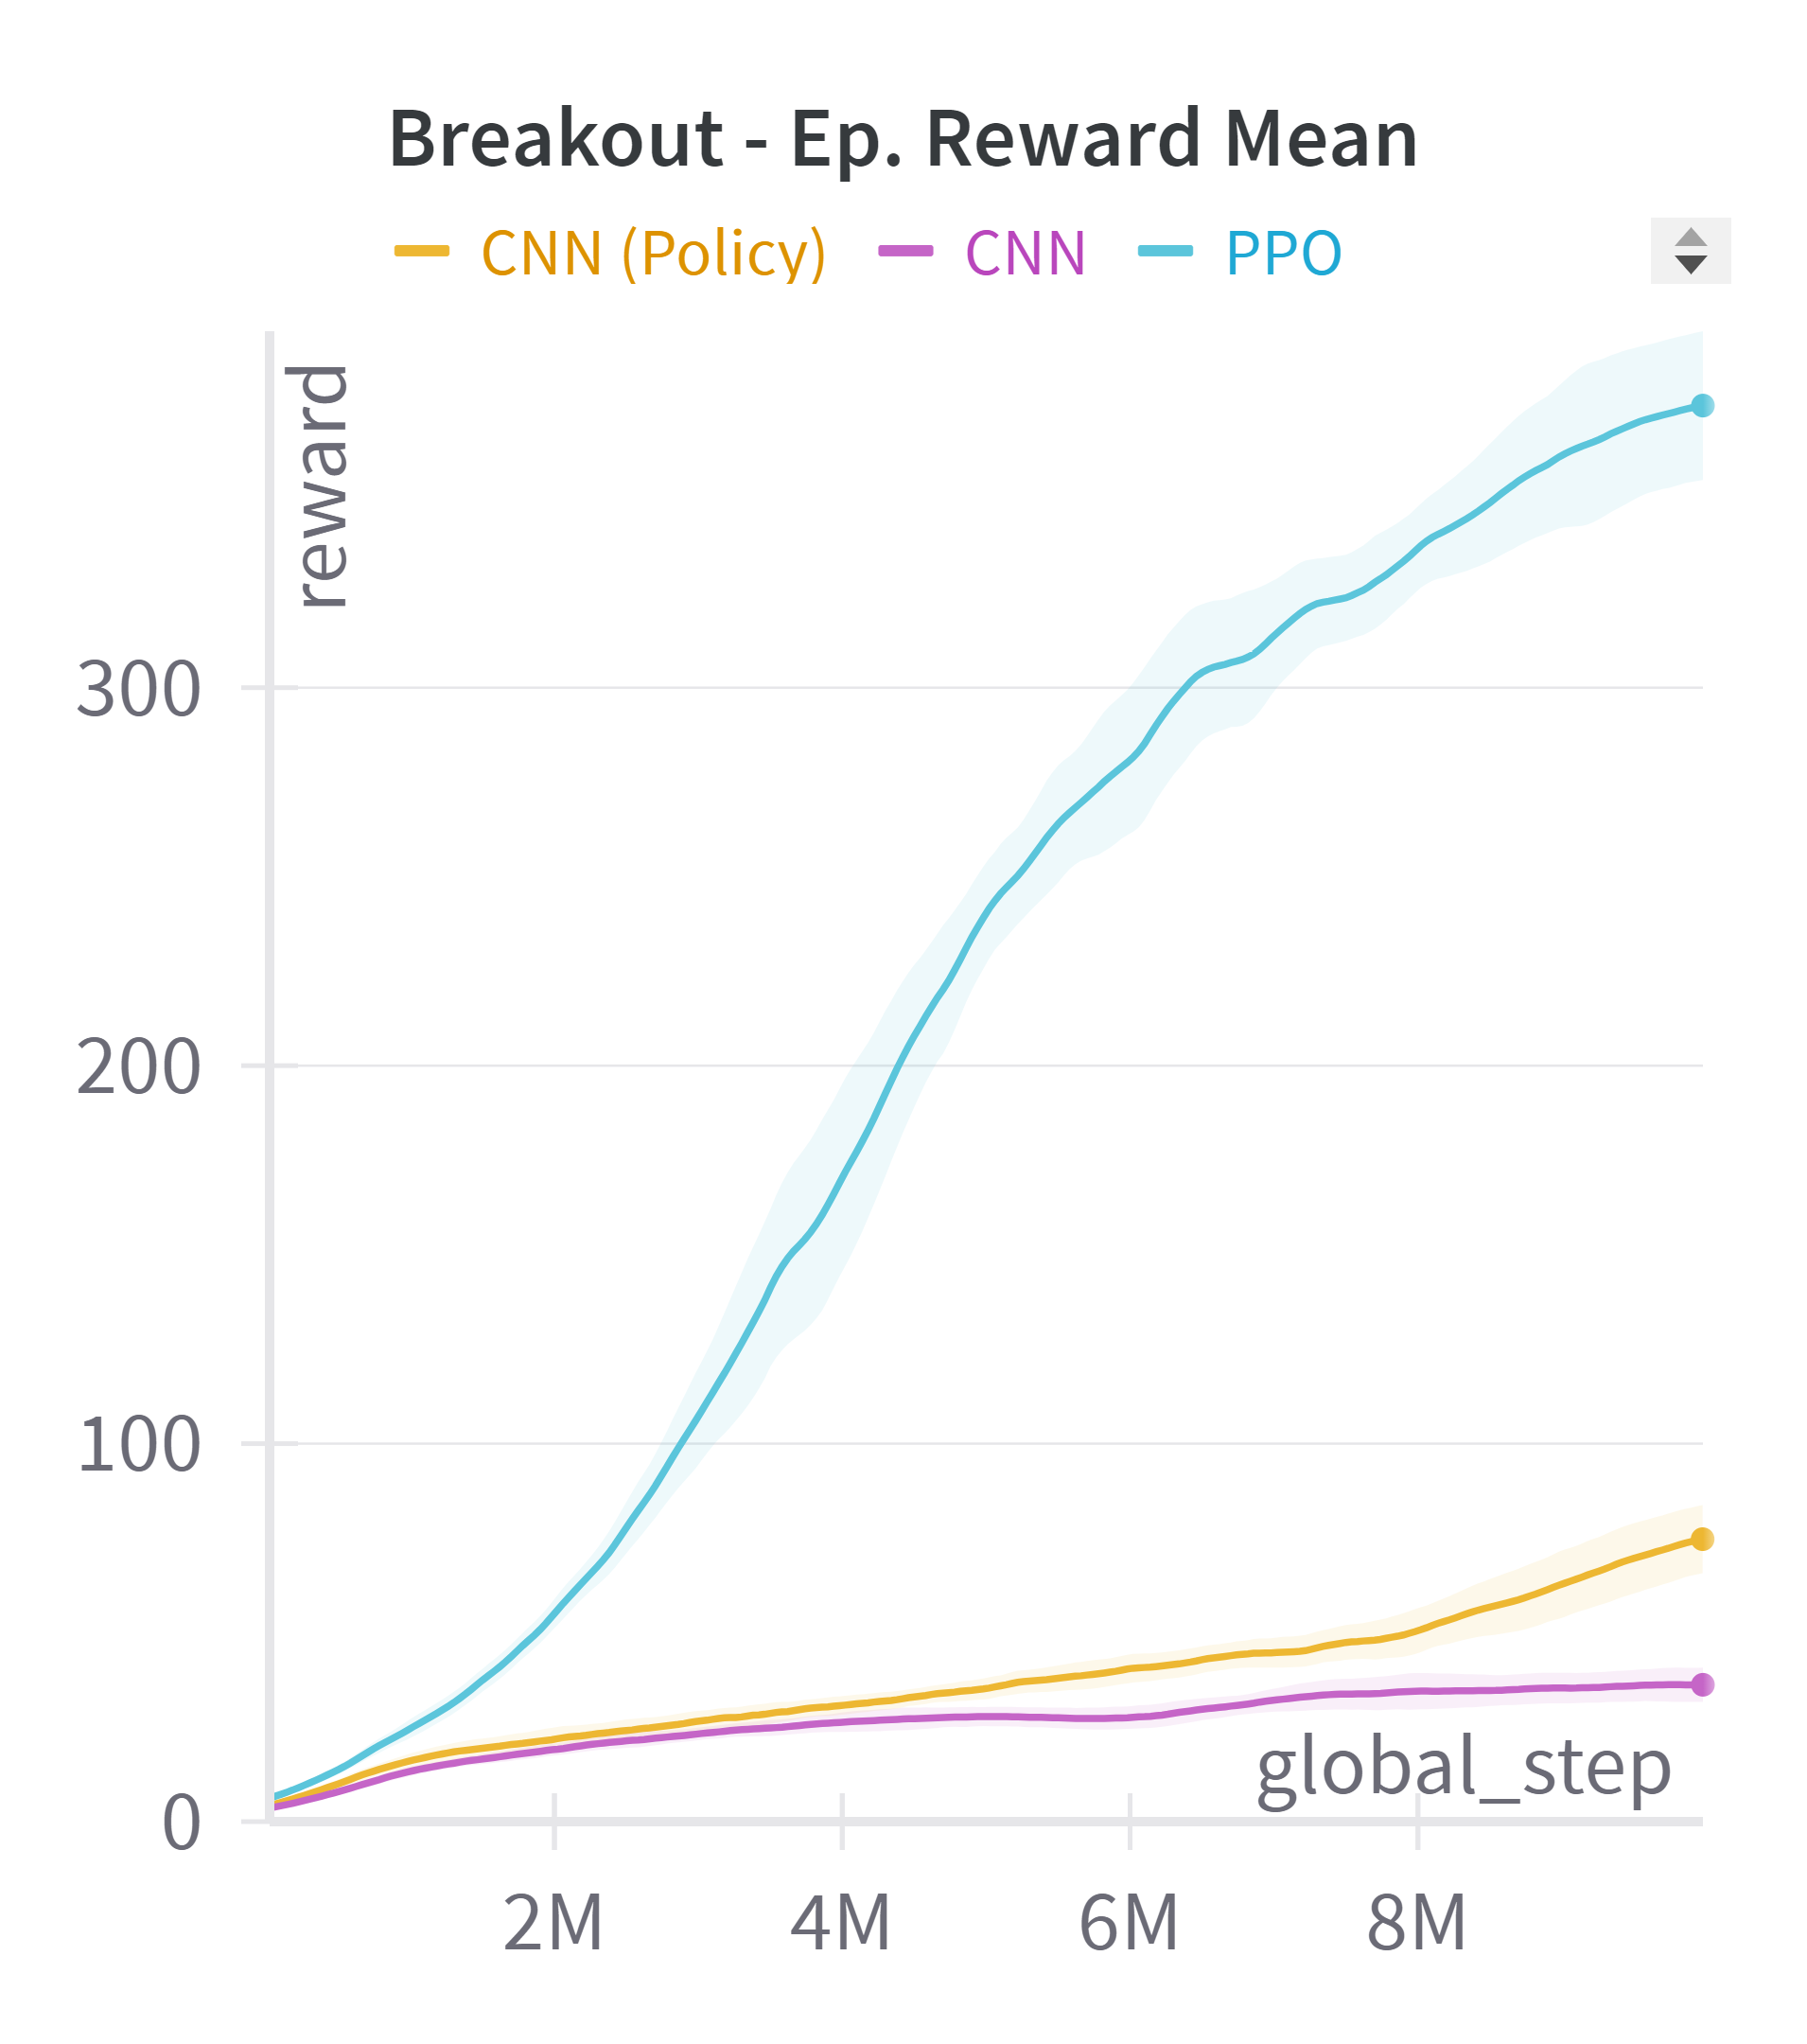
\includegraphics[width=\textwidth]{images/breakout_cnn_policy}
        \caption{Increasing MLP size}
        \label{fig:breakout_cnn_policy}
    \end{subfigure}
    \hfill
    \begin{subfigure}[b]{0.32\textwidth}
        \centering
        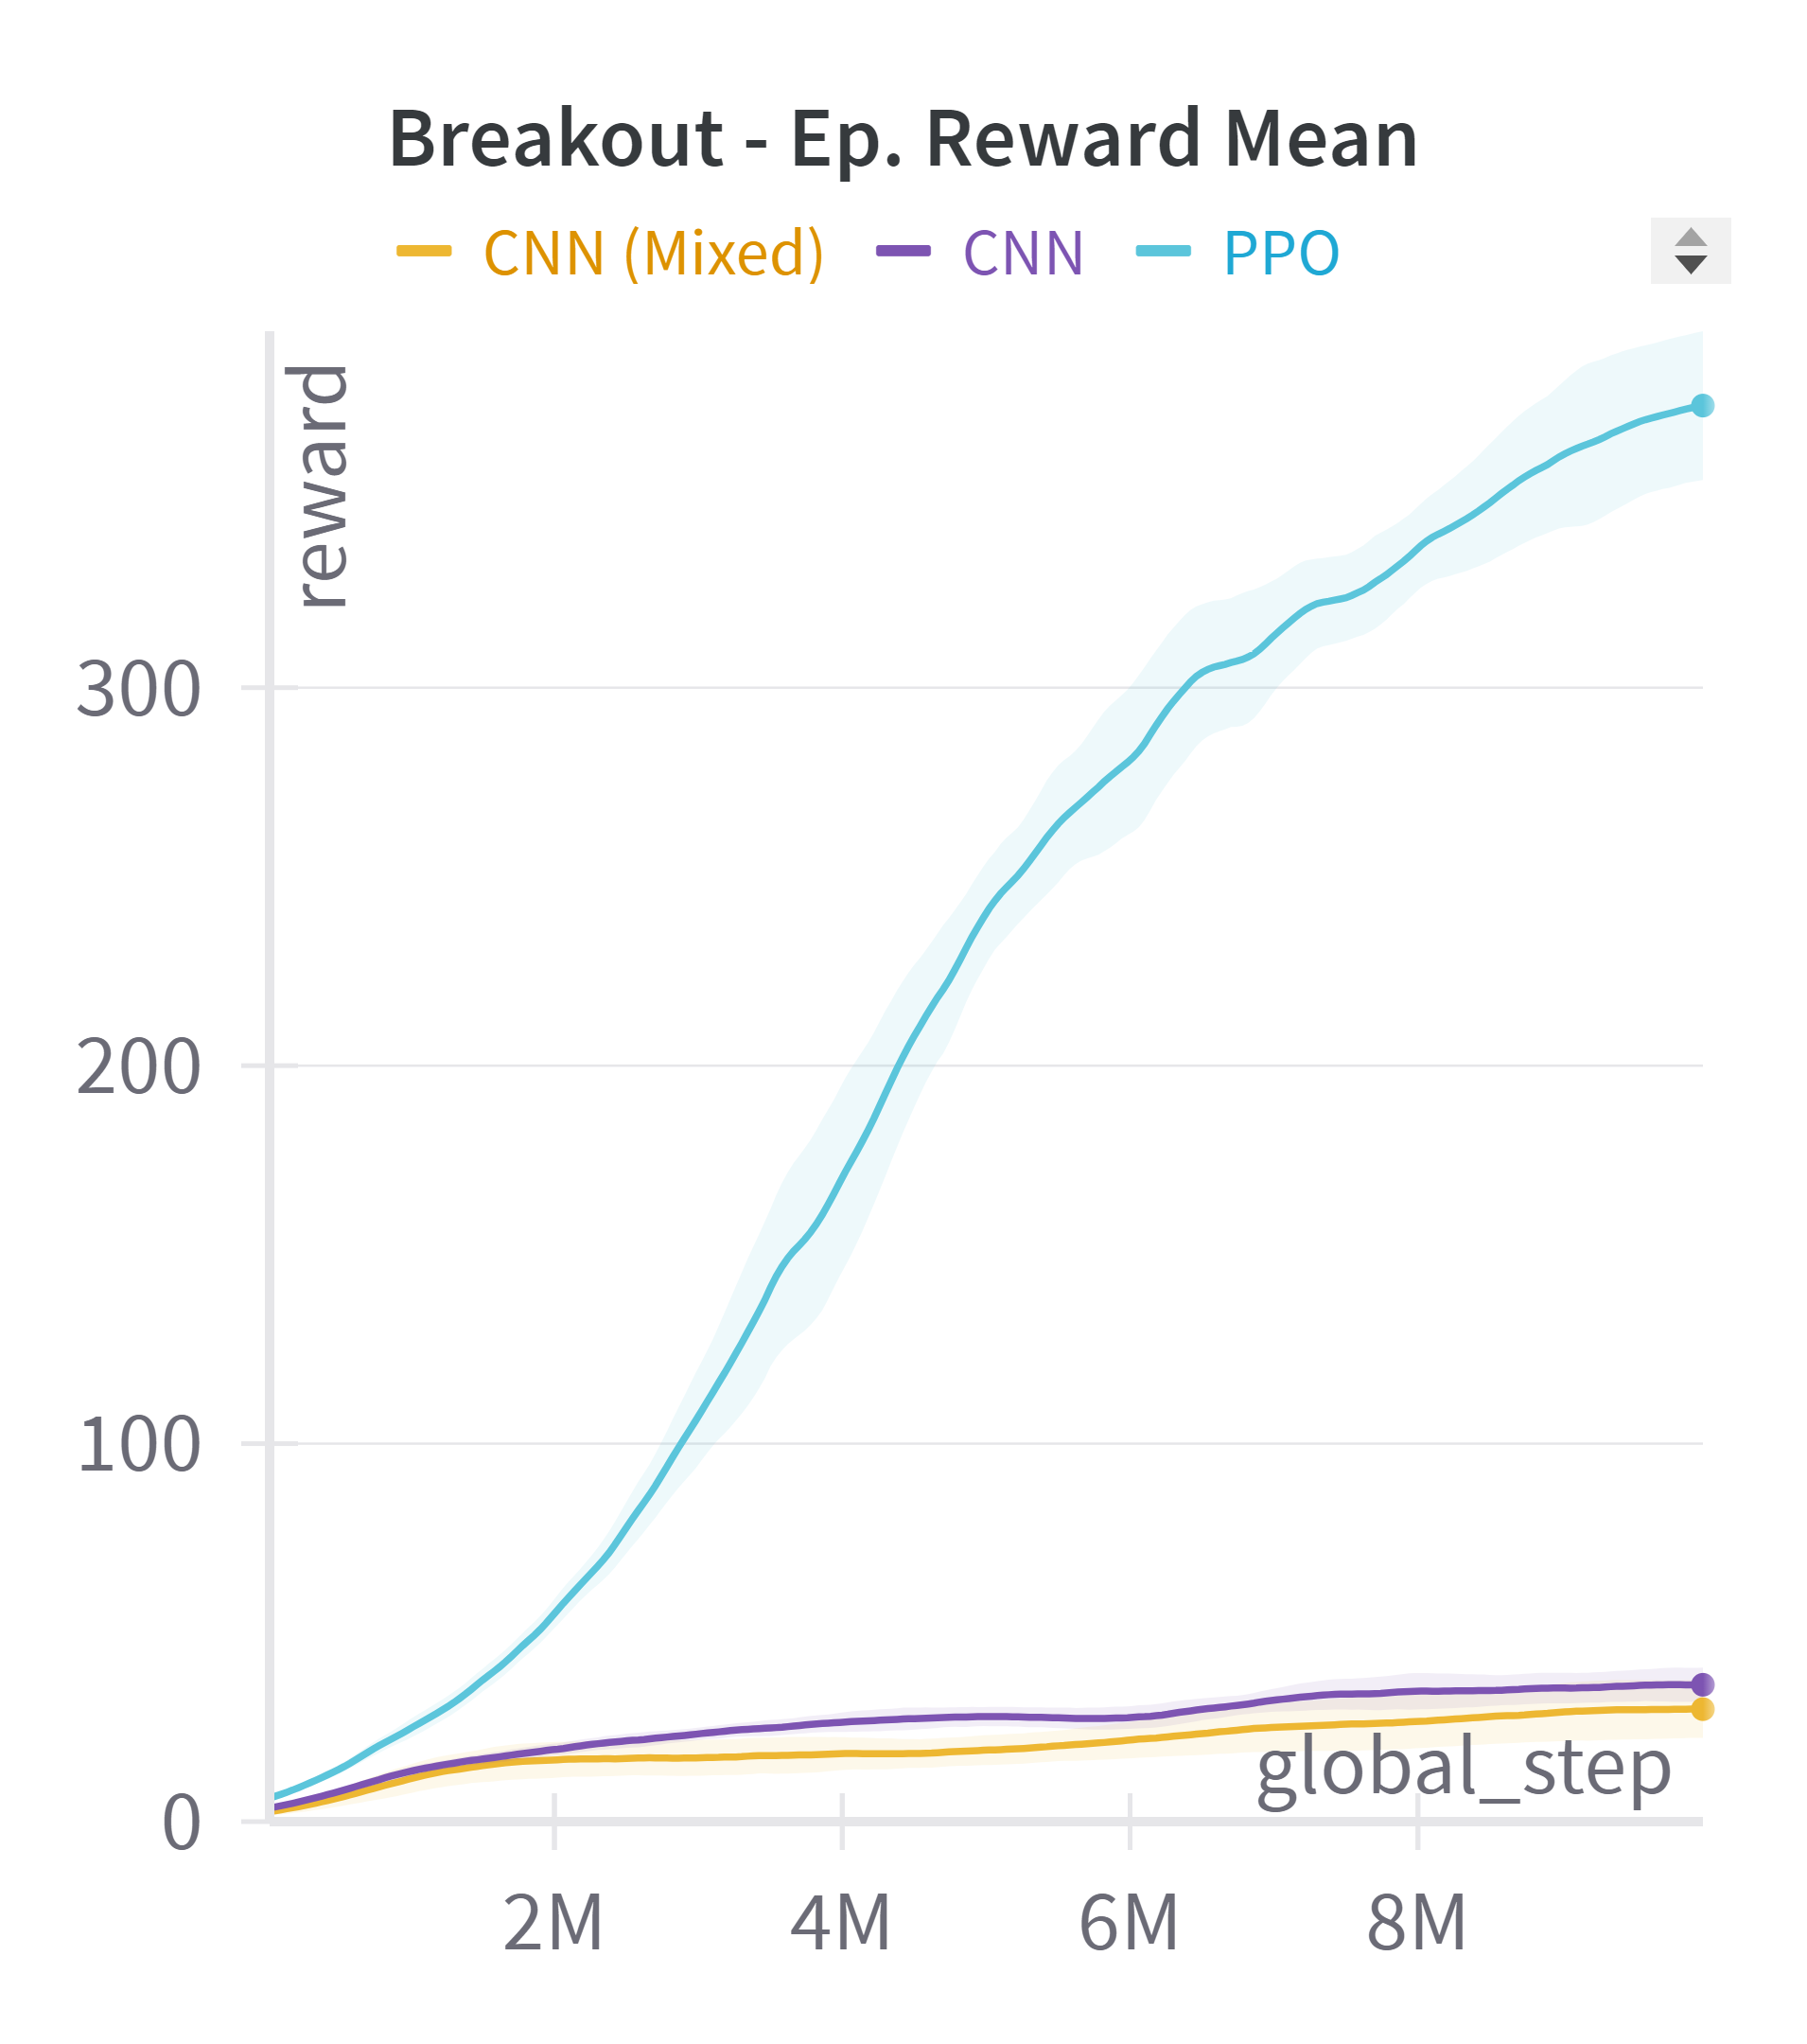
\includegraphics[width=\textwidth]{images/breakout_cnn_mixed}
        \caption{Using Mixed Data}
        \label{fig:breakout_cnn_mixed}
    \end{subfigure}
    \hfill
    \begin{subfigure}[b]{0.32\textwidth}
        \centering
        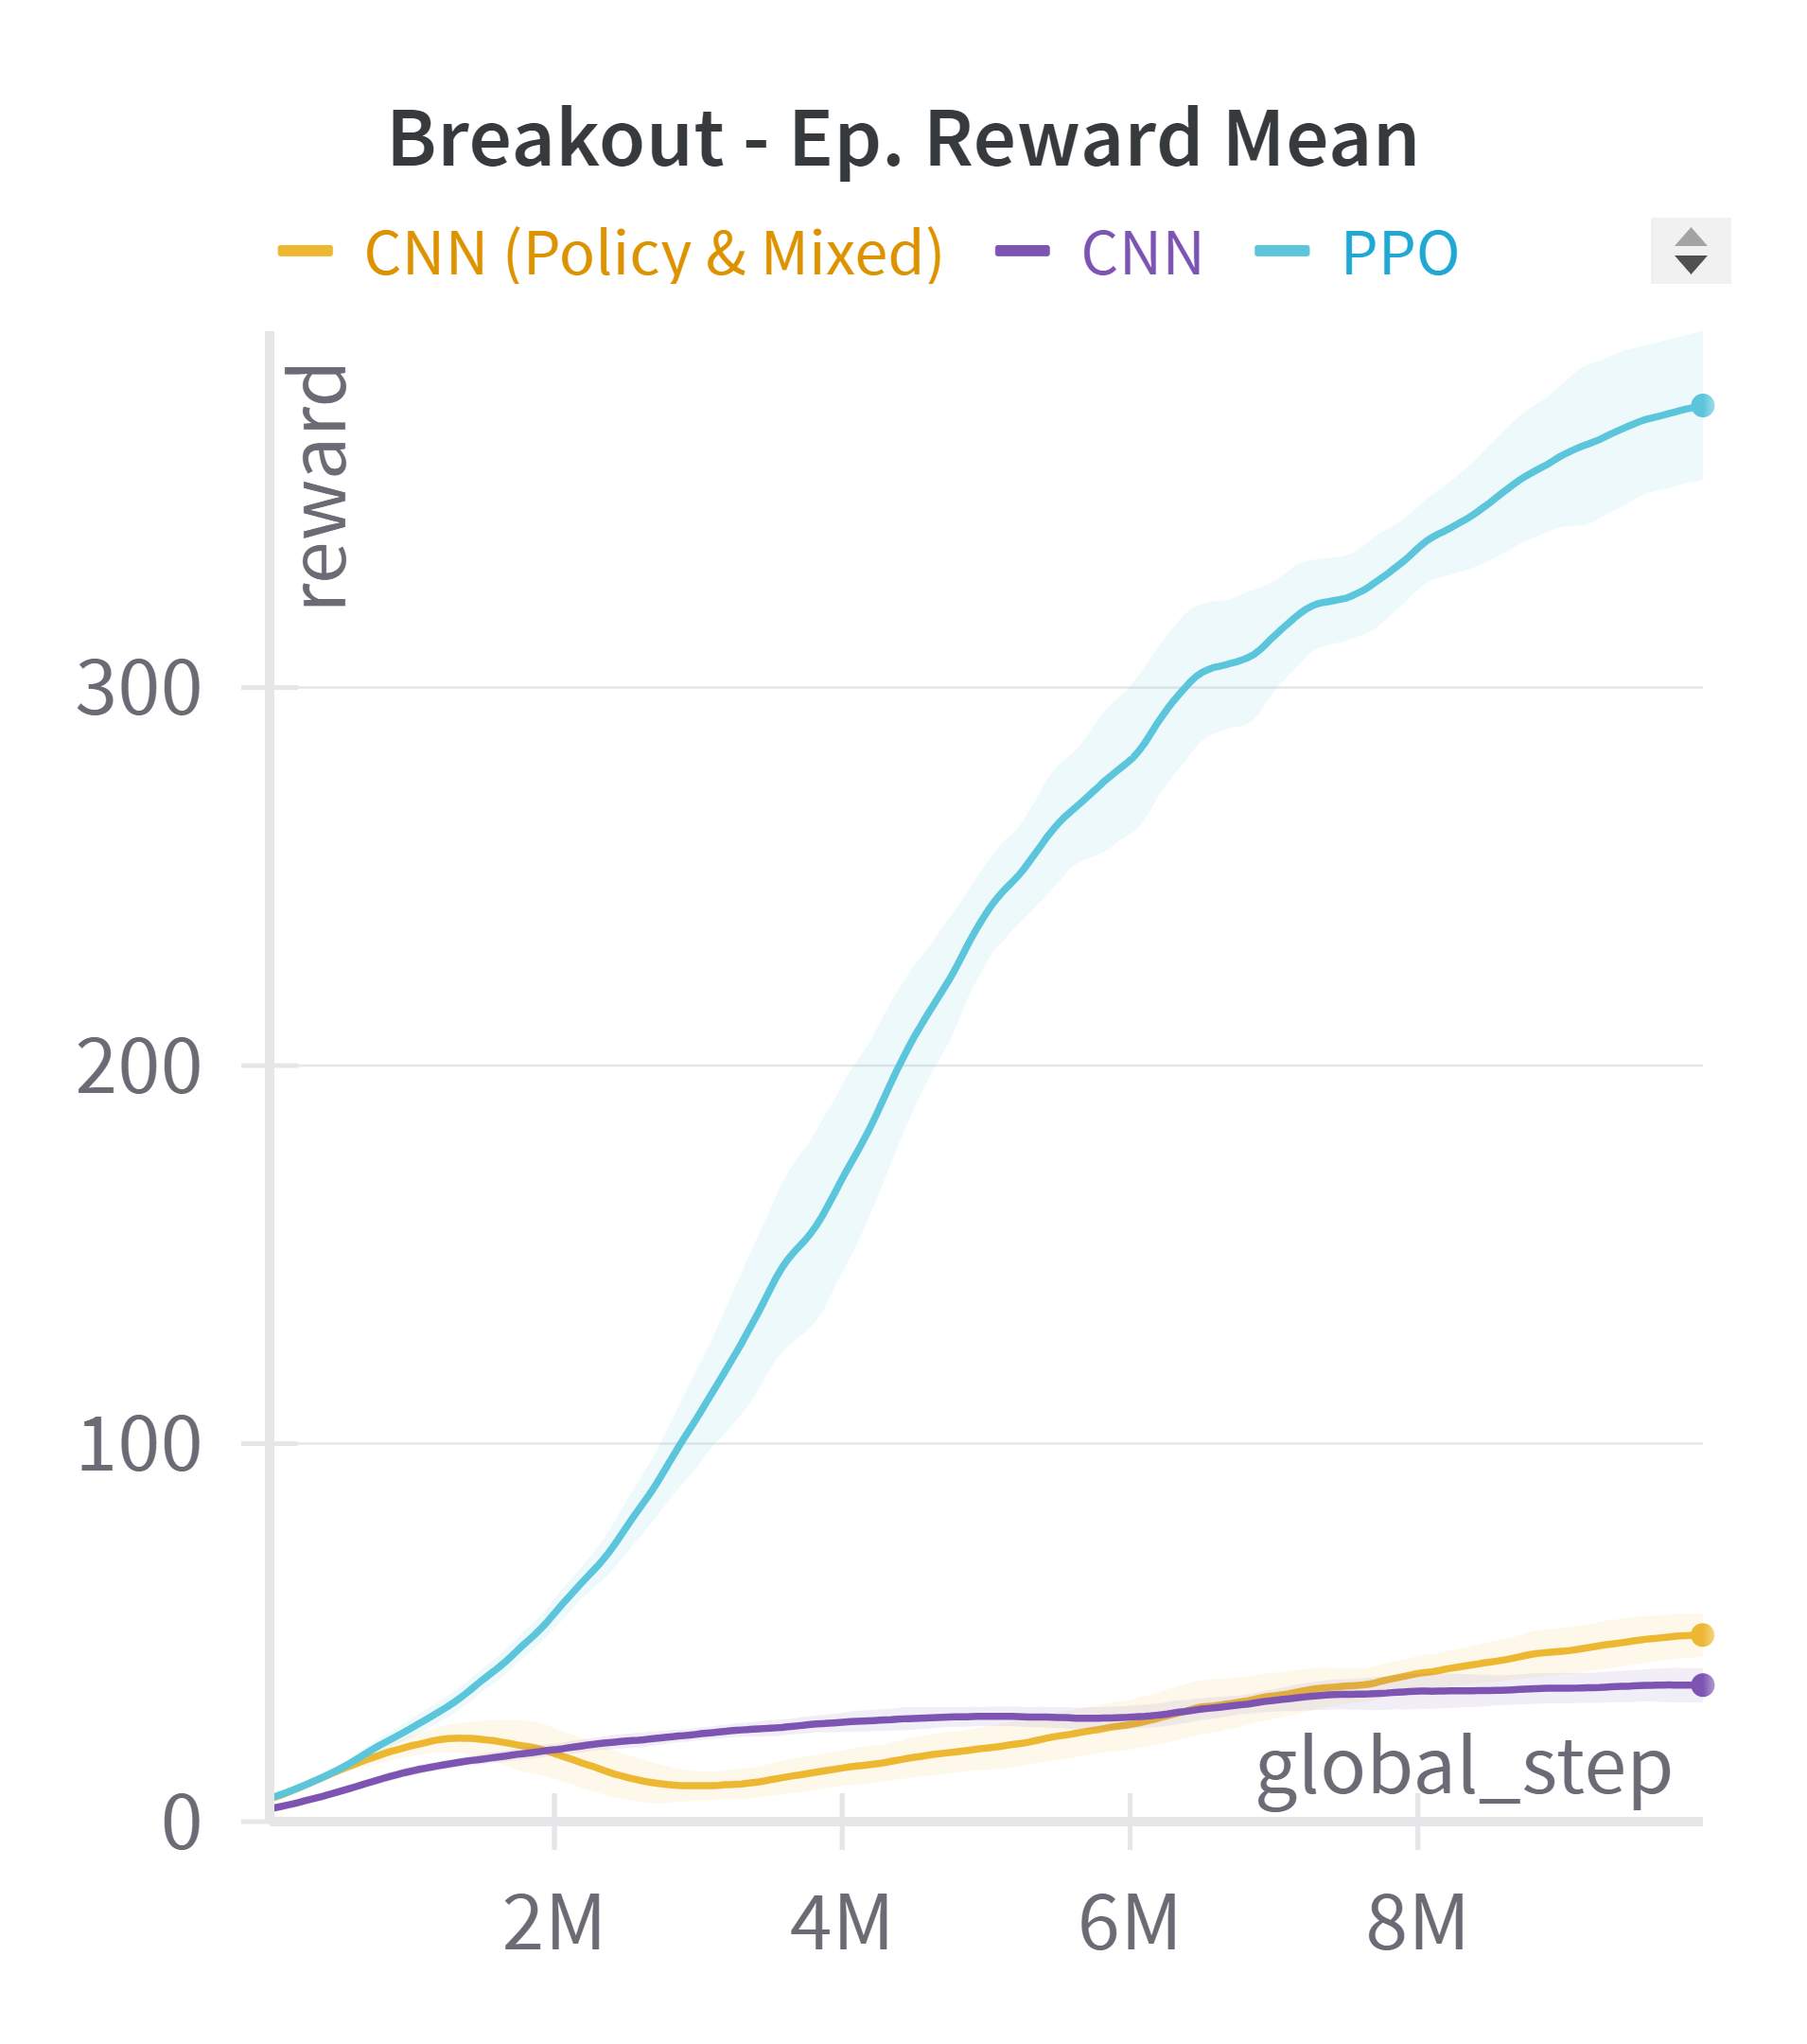
\includegraphics[width=\textwidth]{images/breakout_cnn_policy_mixed}
        \caption{Mixed Data + Increased MLP}
        \label{fig:breakout_cnn_expert_policy}
    \end{subfigure}
    \caption{Performance comparison of CNN with PPO across various strategies on \textit{Breakout}. Each subfigure displays the average score with the standard deviation shaded.}
    \label{fig:breakout_cnn_study}
\end{figure}

\begin{figure}[ht]
    \centering
    \begin{subfigure}[b]{0.32\textwidth}
        \centering
        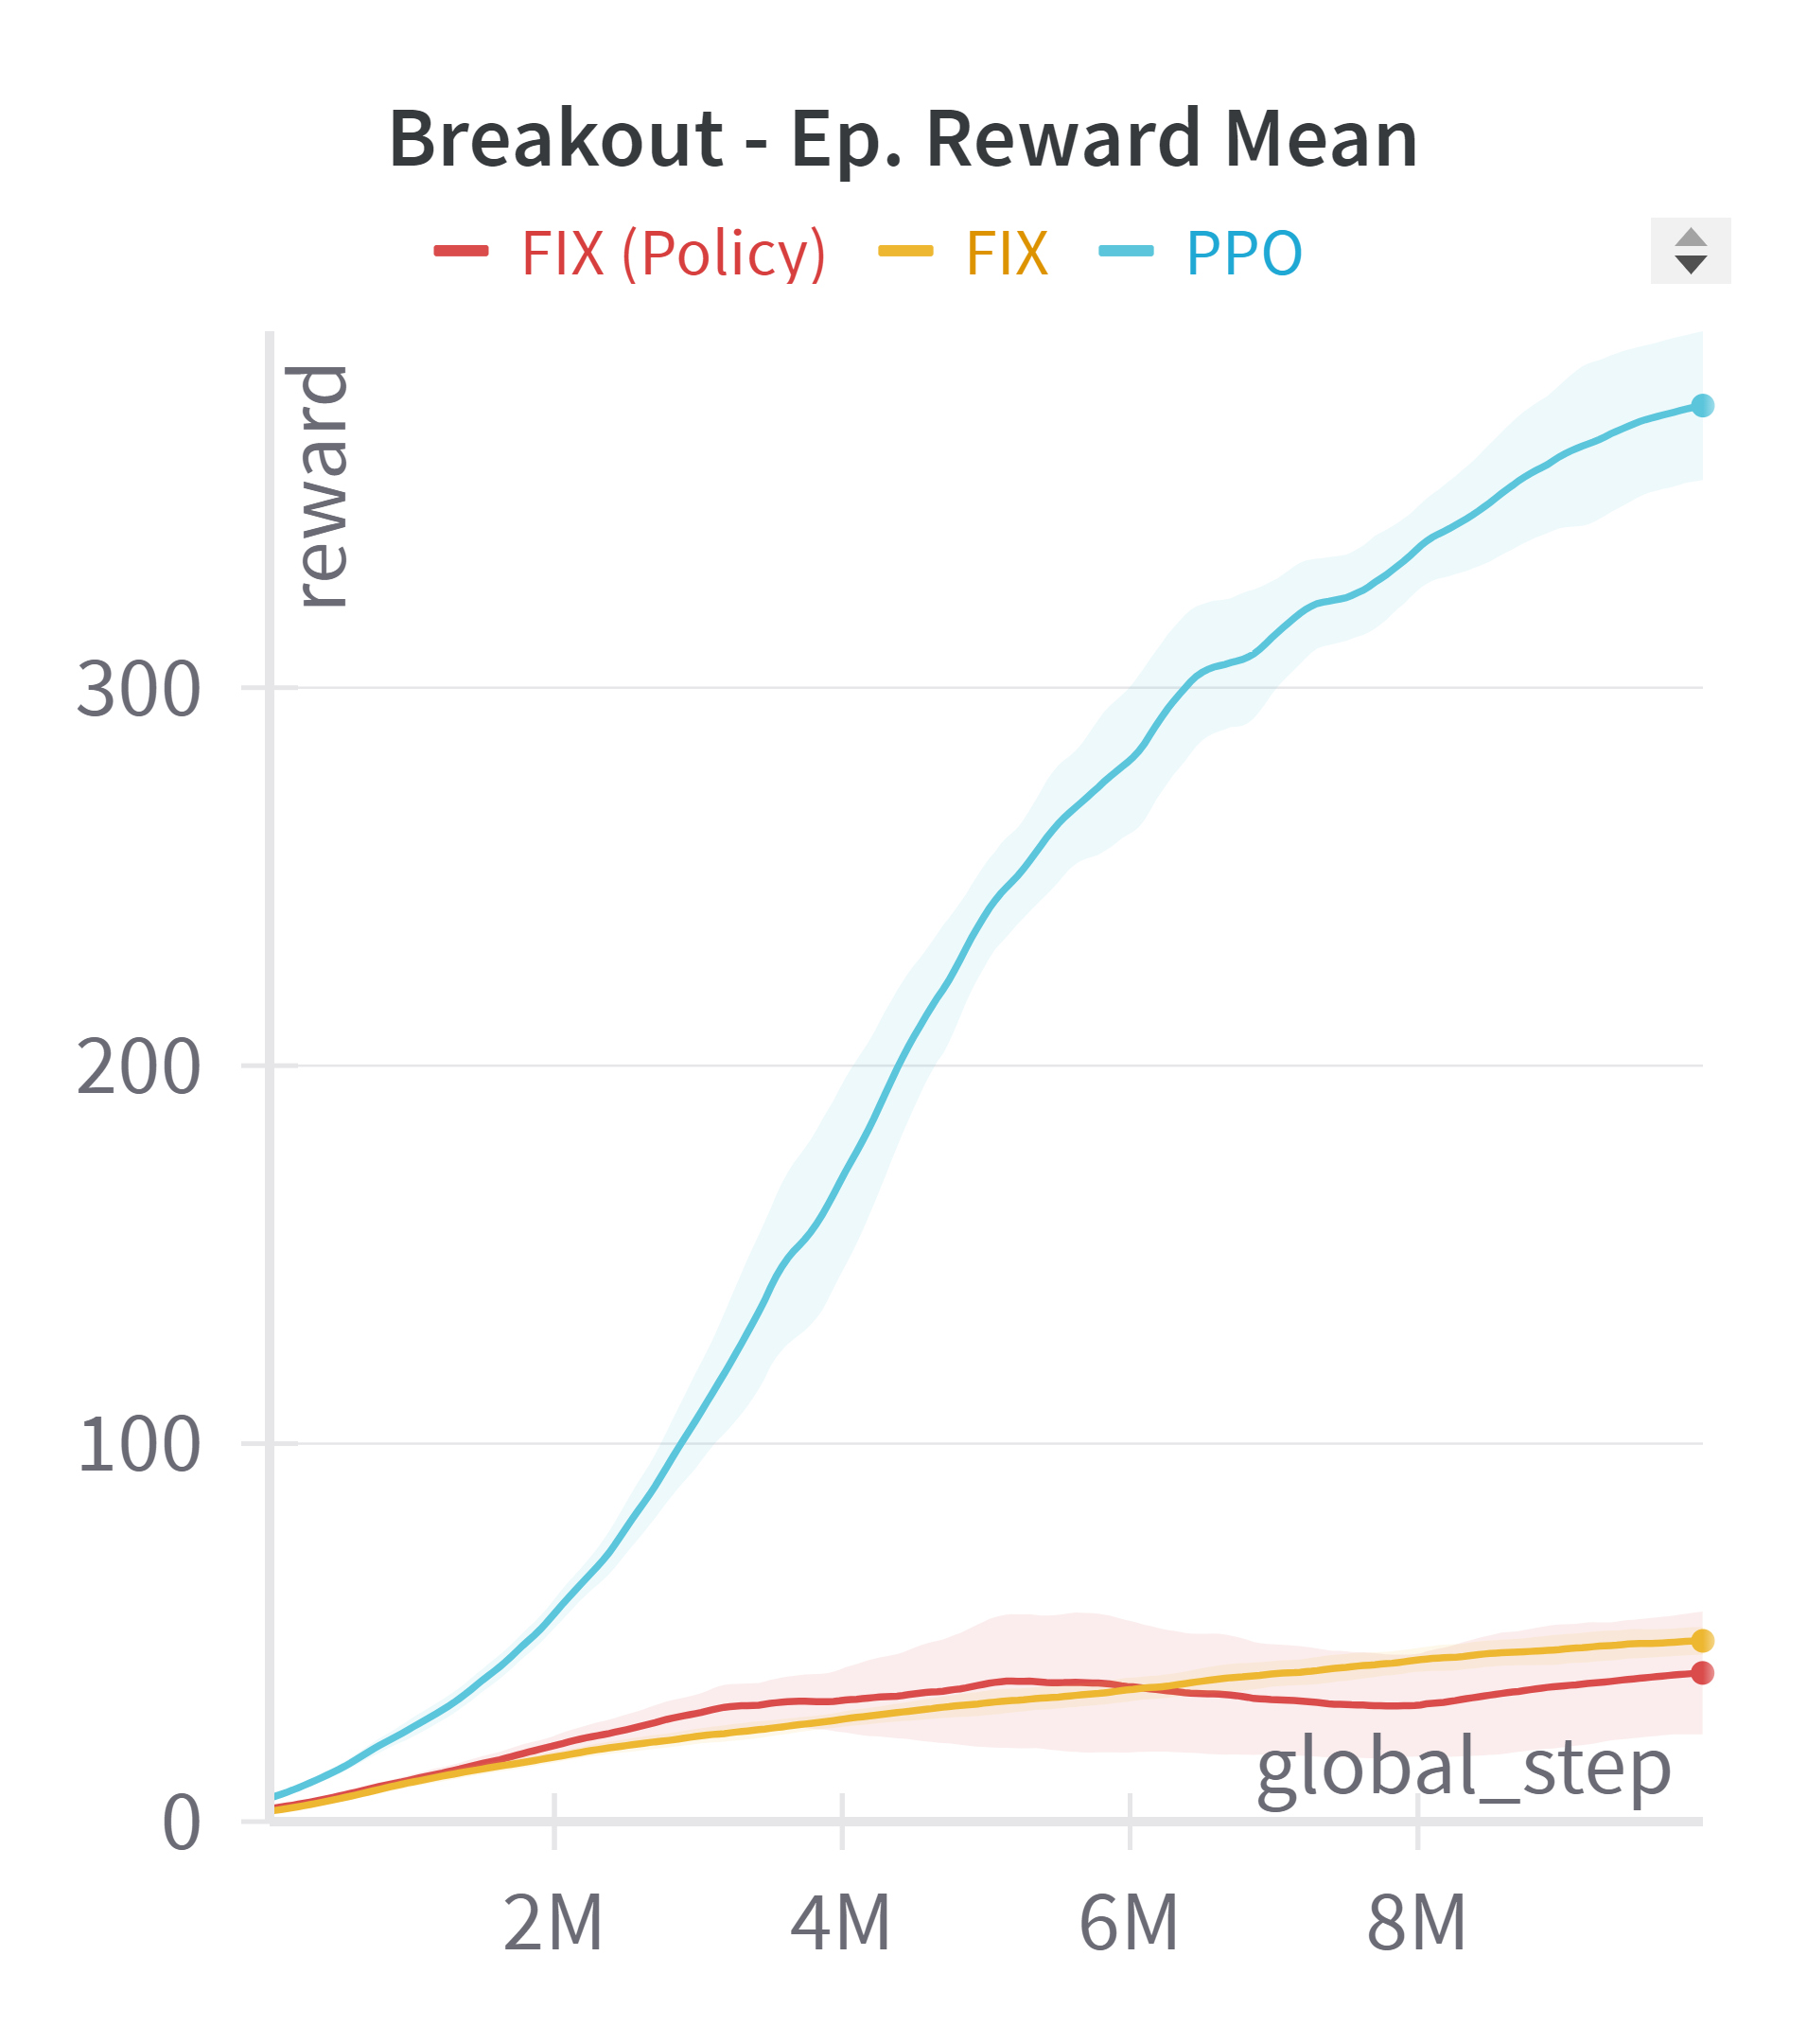
\includegraphics[width=\textwidth]{images/breakout_fix_policy}
        \caption{Increasing MLP size}
        \label{fig:breakout_fix_policy}
    \end{subfigure}
    \hfill
    \begin{subfigure}[b]{0.32\textwidth}
        \centering
        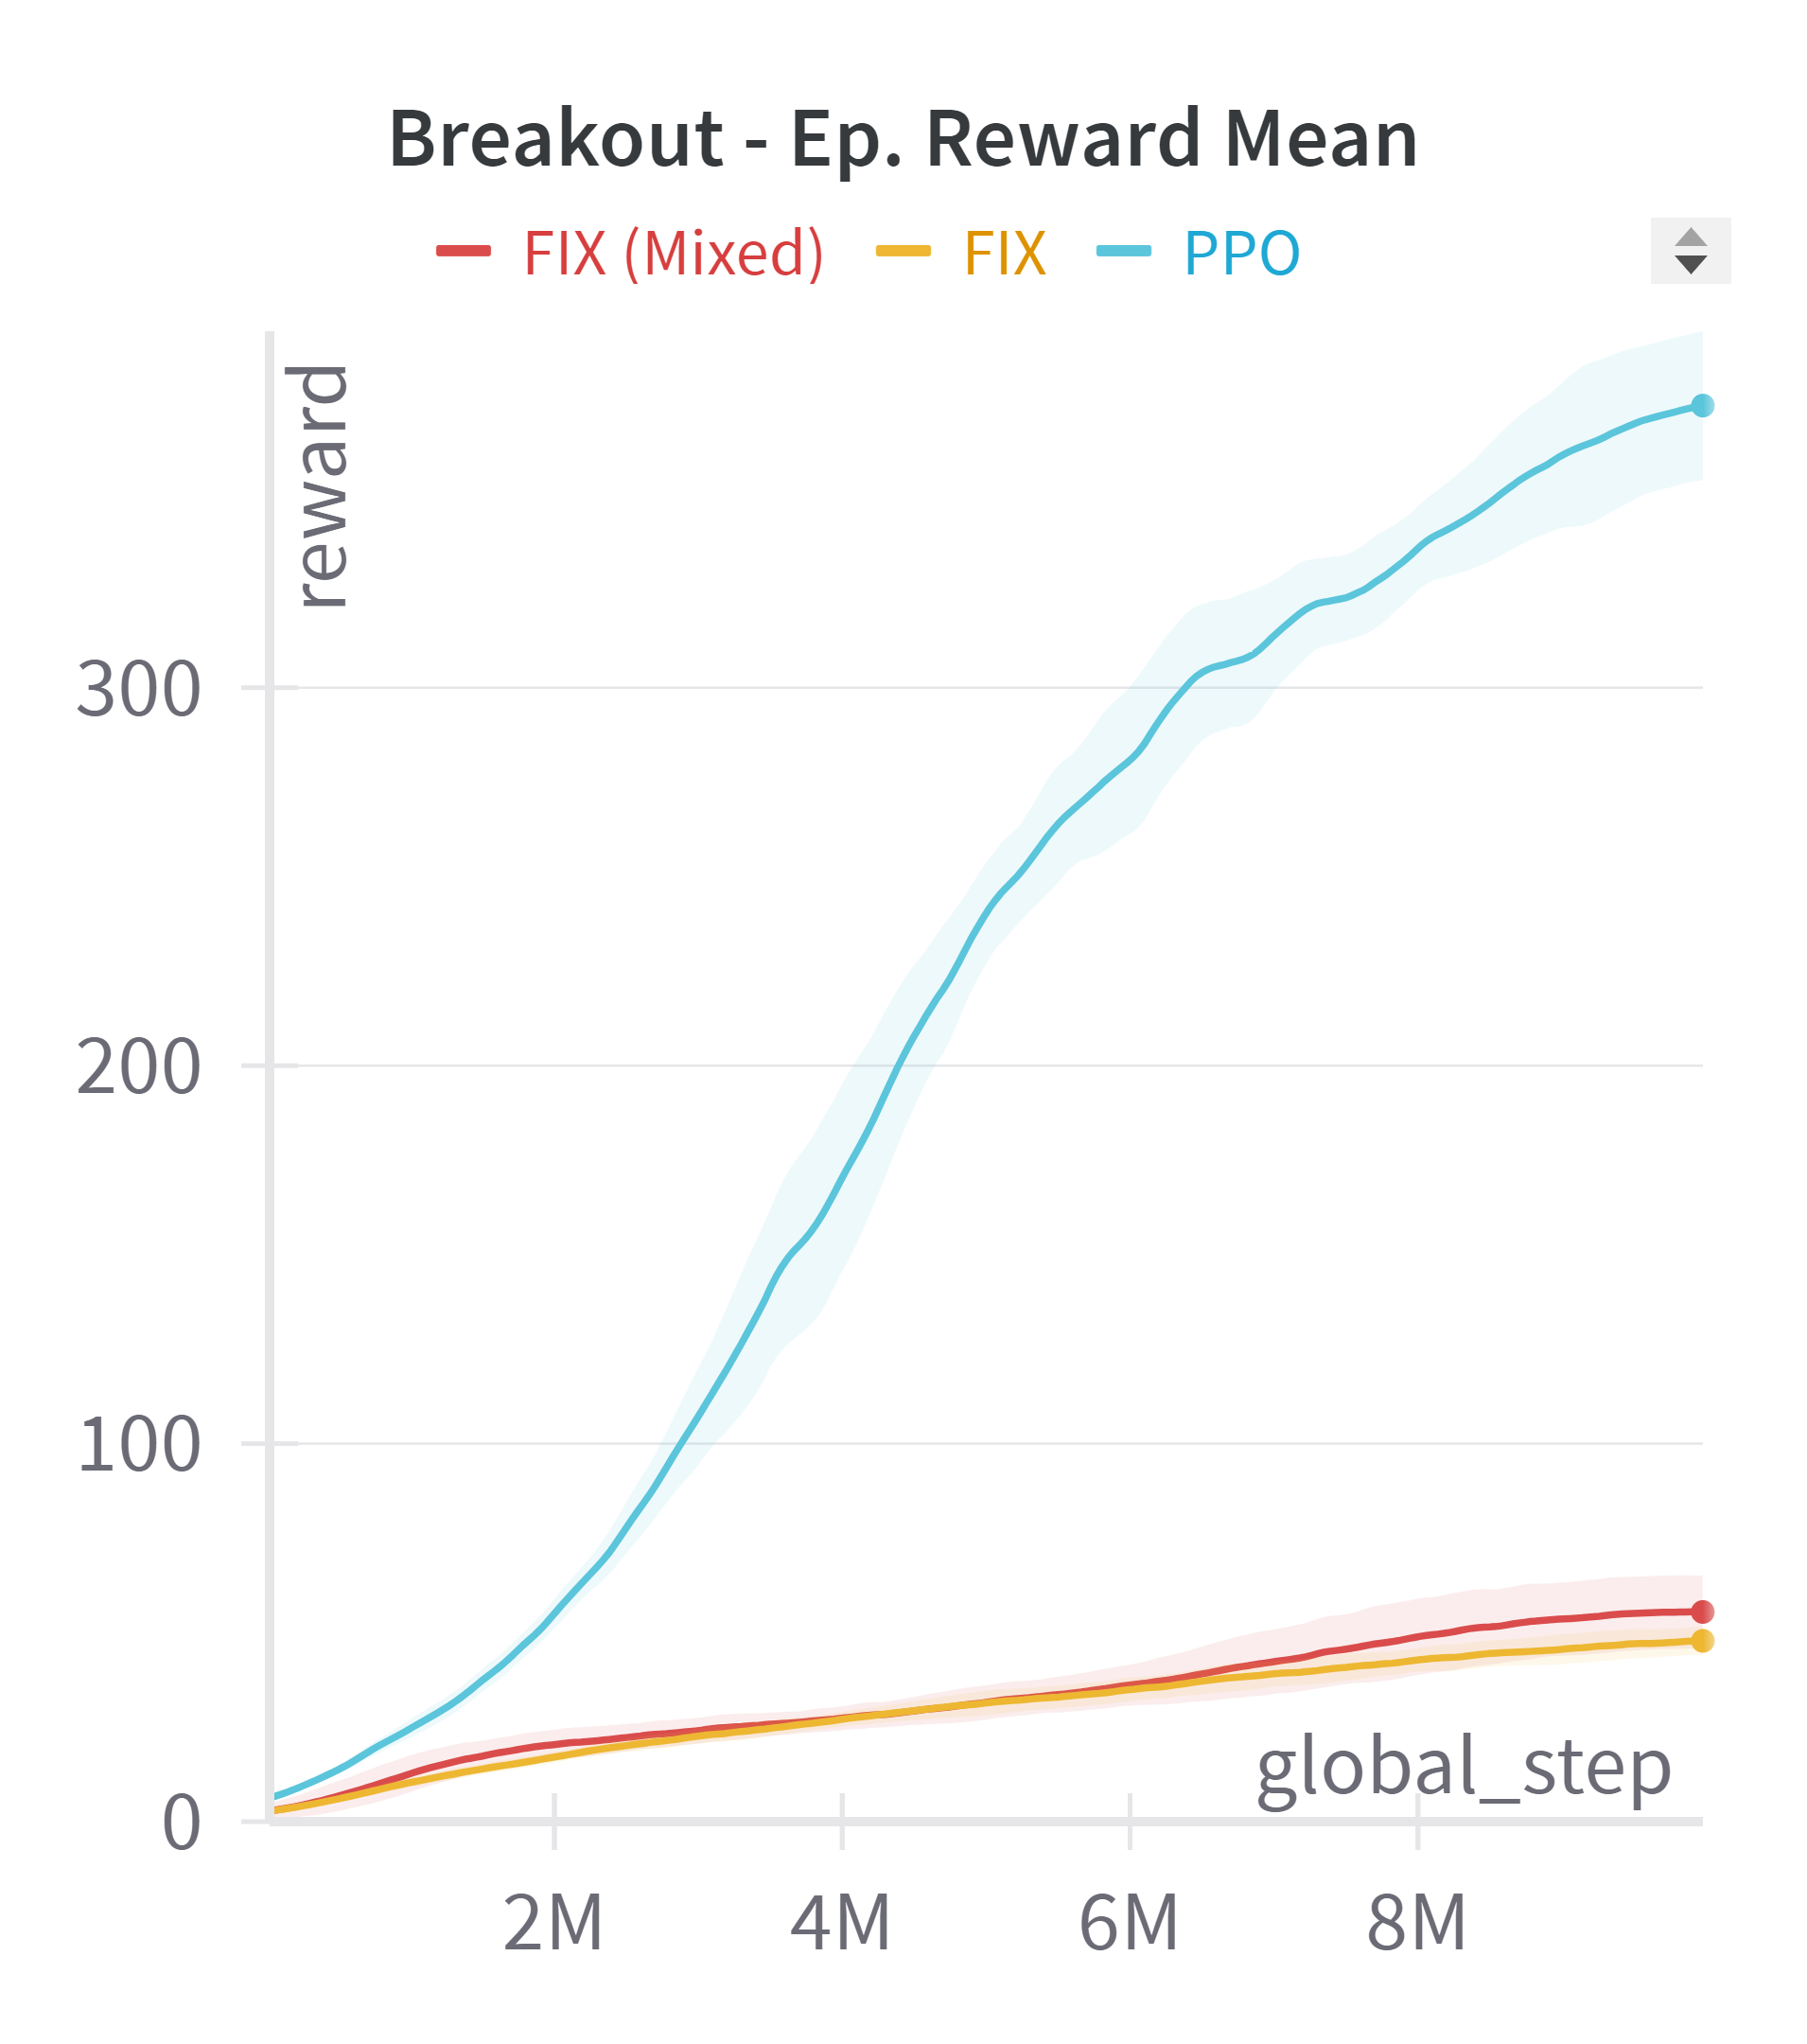
\includegraphics[width=\textwidth]{images/breakout_fix_mixed}
        \caption{Using Mixed Data}
        \label{fig:breakout_fix_mixed}
    \end{subfigure}
    \hfill
    \begin{subfigure}[b]{0.32\textwidth}
        \centering
        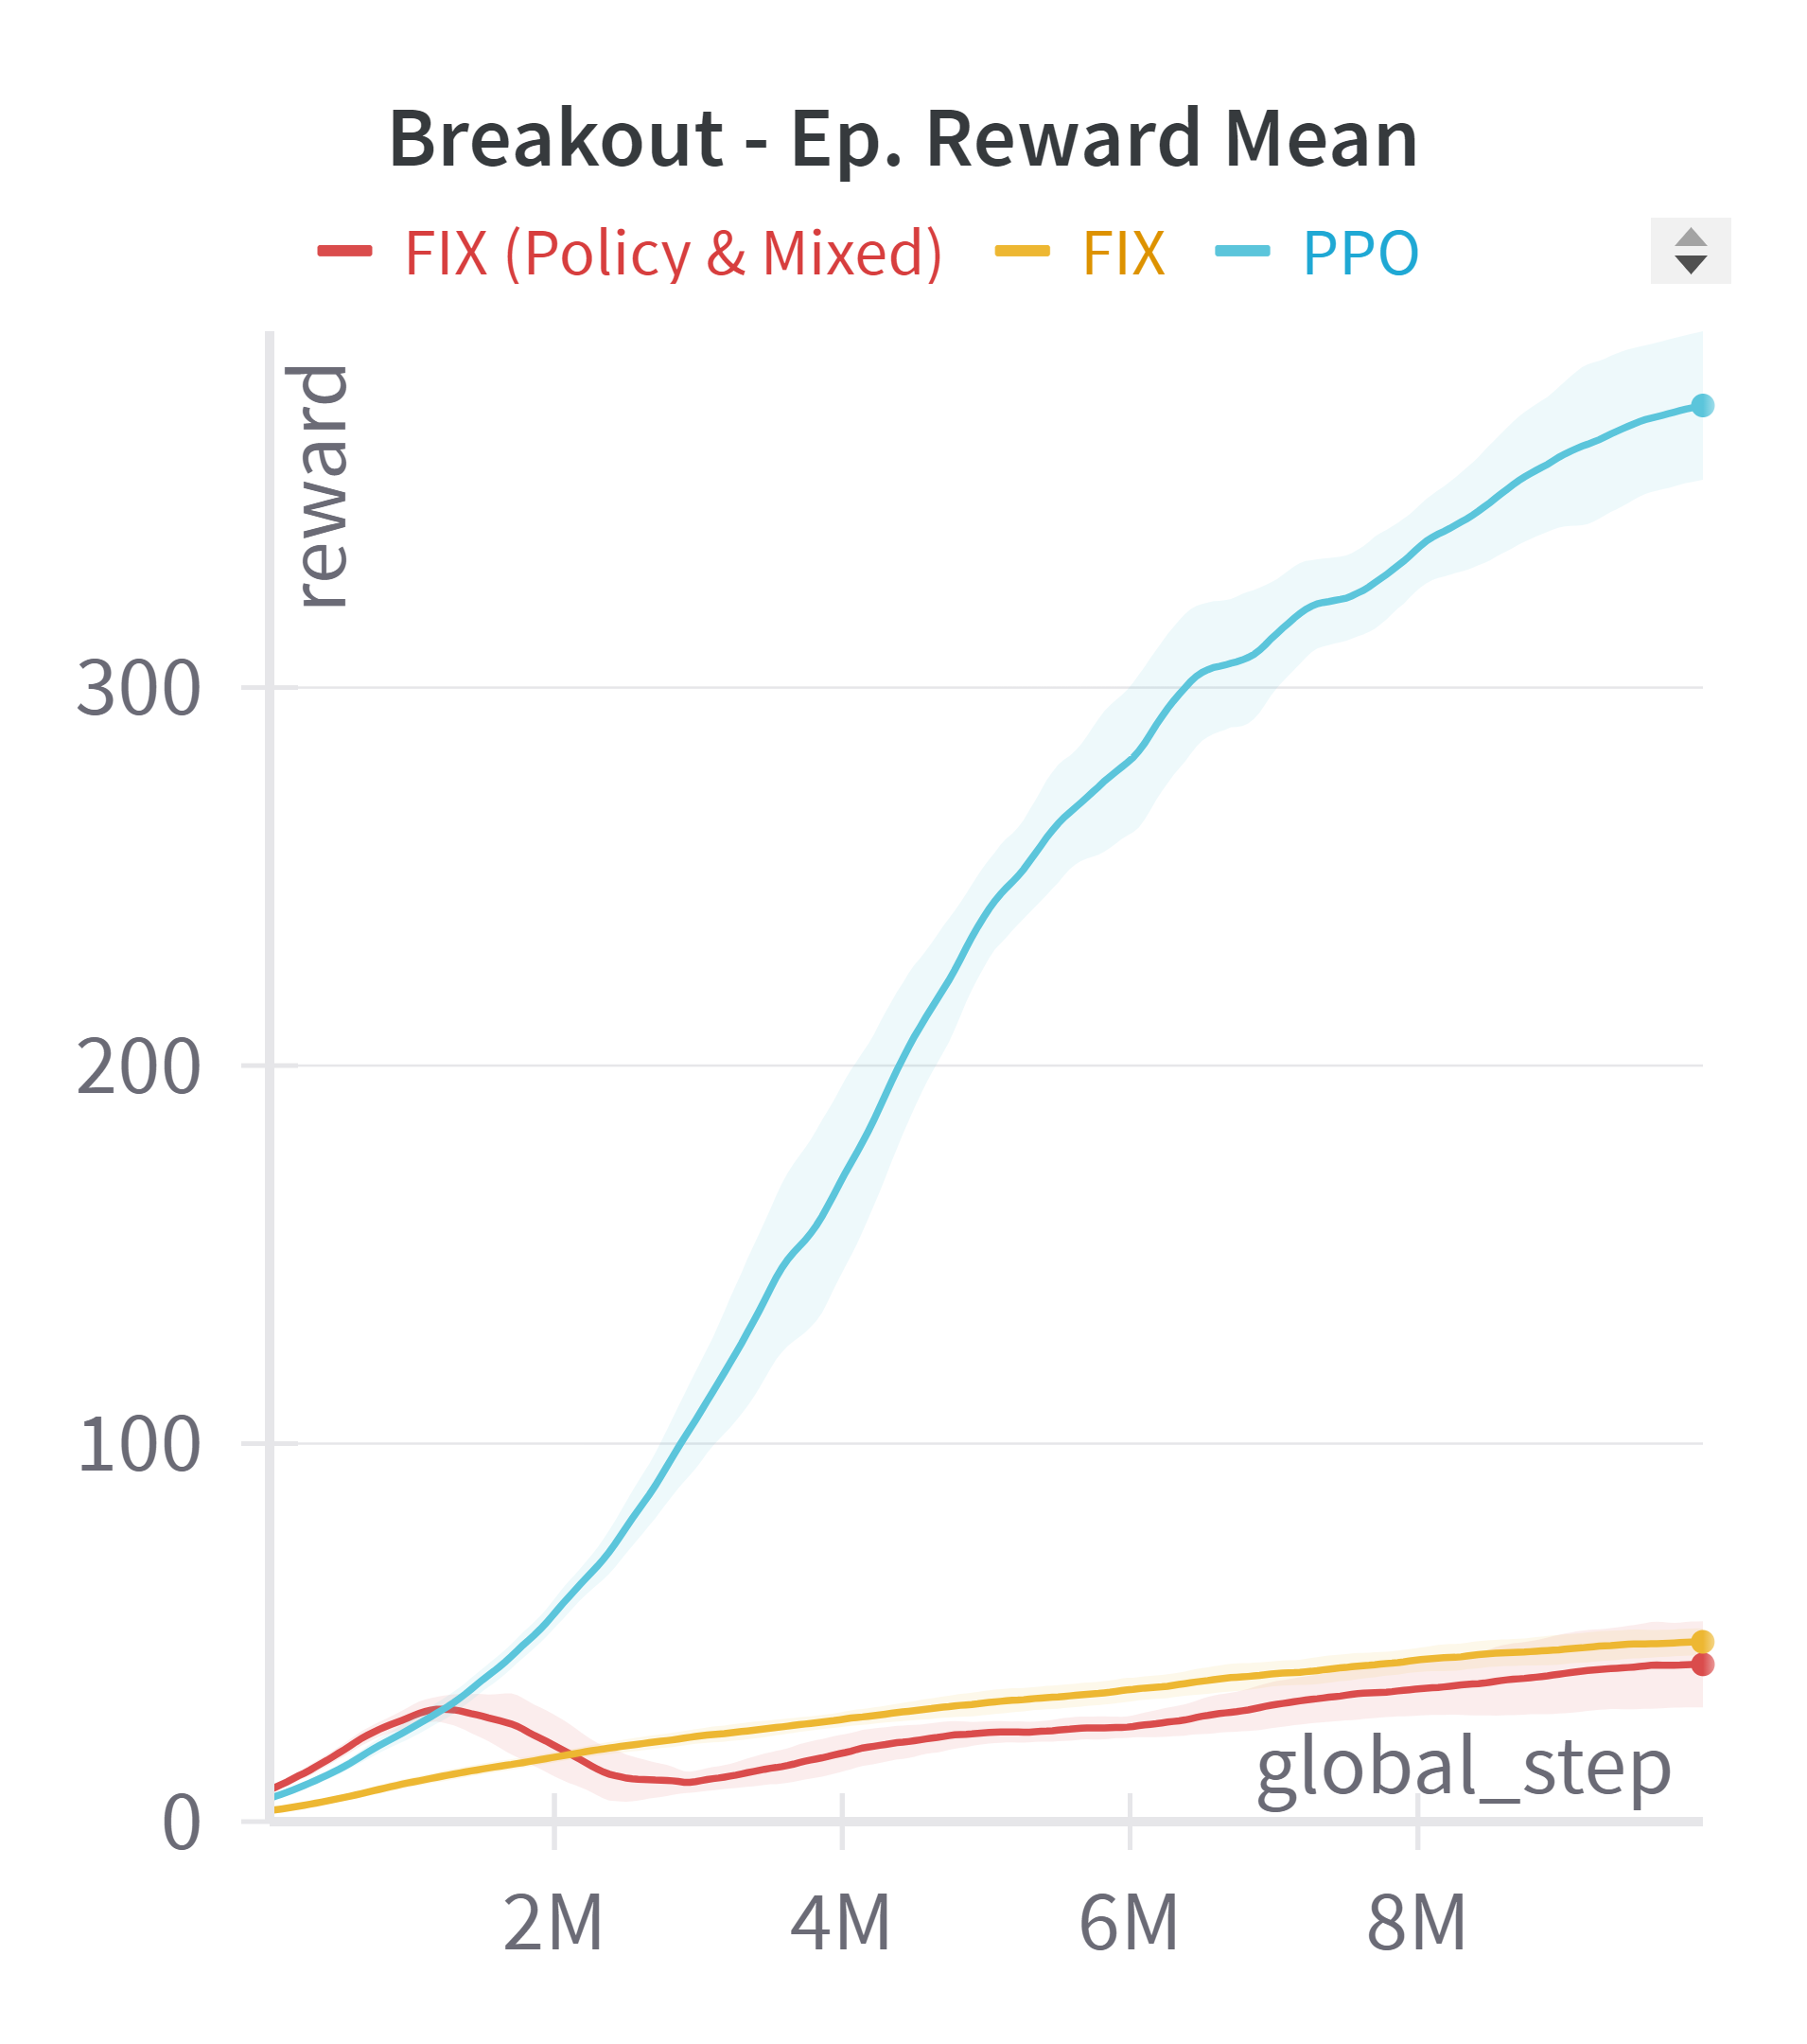
\includegraphics[width=\textwidth]{images/breakout_fix_policy_mixed}
        \caption{Mixed Data + Increased MLP}
        \label{fig:breakout_fix_expert_policy}
    \end{subfigure}
    \caption{Performance comparison of FIX with PPO across various strategies on \textit{Breakout}. Each subfigure displays the average score with the standard deviation shaded.}
    \label{fig:breakout_fix_study}
\end{figure}


\begin{table}[ht]
\centering
    \begin{tabular}[b]{lll}
                \multicolumn{1}{l}{Environment}  &\multicolumn{1}{l}{\textbf{Agent}} &\multicolumn{1}{l}{\textbf{Reward}} \\
                \hline \\


                \multirow{3}{*}{\texttt{Breakout}}
                                      & CNN & 65.98 $\pm$ 1.62 \\
                                      & FIX & 87.17 $\pm$ 6.87 \\
                                      & WSA & 99.58 $\pm$ 6.66 \\

                \multirow{3}{*}{\texttt{Breakout - Policy}}
                                      & CNN & 118.71 $\pm$ 4.30 \\
                                      & FIX & 106.46 $\pm$ 10.84 \\
                                      & WSA & 156.17 $\pm$ 3.59 \\

                \multirow{3}{*}{\texttt{Breakout - Mixed}}
                                      & CNN & 62.21 $\pm$ 1.98 \\
                                      & \underline{FIX} & \underline{199.08 $\pm$ 7.46}\\
                                      & WSA & 345.52 $\pm$ 6.47 \\

                \multirow{4}{*}{\texttt{Breakout - Policy \& Mixed}}
                                      & CNN & 68.51 $\pm$ 1.85 \\
                                      & FIX & 71.06 $\pm$ 5.04 \\
                                      & \underline{WSA} & \underline{387.15 $\pm$ 0.43} \\ \\


                                      & \textbf{PPO} & \textbf{413.51 $\pm$ 1.10}\\
    \end{tabular}
    \caption{TODO}
    \label{tab:breakout_results}
\end{table}

As final note, it is important to underline that we conducted these experiments considering only the top-performing modules for each game highlighted in Section~\ref{sec:top-3-performer} and we did not test again all the combination modules with different configurations.


\section{Weight Sharing Attention Explainability}\label{sec:explainability}

%%In most of the experiments we have performed, we have noticed that weights sharing attention as a way of concatenating different skill embeddings is the one that performs best.
%%It, being more general as a method manages to better filter out noisy input, focusing only on the information that is really important for the agent to learn.

In this Section we provide an analysis of the explainability of the WSA module.
In fact, thanks to the nature of attention mechanism, we can analyze the weights assigned to each pre-trained model in different scenarios.
This can provide insights on how the agent uses the FMs to make decisions and how the agent adapts its prior knowledge to the environment.
Figure~\ref{fig:breakout_attention} shows the attention weights assigned by the WSA module to each pre-trained model during the evaluation phase of the agent on \textit{Breakout}.
The frames depict also the current frame of the game and the chosen action by the agent.
We considered two different scenarios, one where the agent is in the early stages of the game with many blocks and one where the agent is in the late stages of the game and needs to be more precise to hit the ball in the right direction.
In the first scenario, we can see how SR and VOS are the most weighted models, meaning that they are the most informative.
In the second scenario, we can see how the agent assigns more weight to OKK and VOS.
Since OKK and VOS track moving objects, most probably they encode more information about the paddle and the ball, and the agent needs this information to make the right decision.
%add more eventually


TODO-DA FINIRE

It is important to notice that the agent considered is the one that performed the best i.e.\ the one trained with mixed data and increased \textit{Fully-Connected Network}.


\begin{figure}[ht]
    \centering
    \begin{subfigure}[b]{0.45\textwidth}
        \centering
        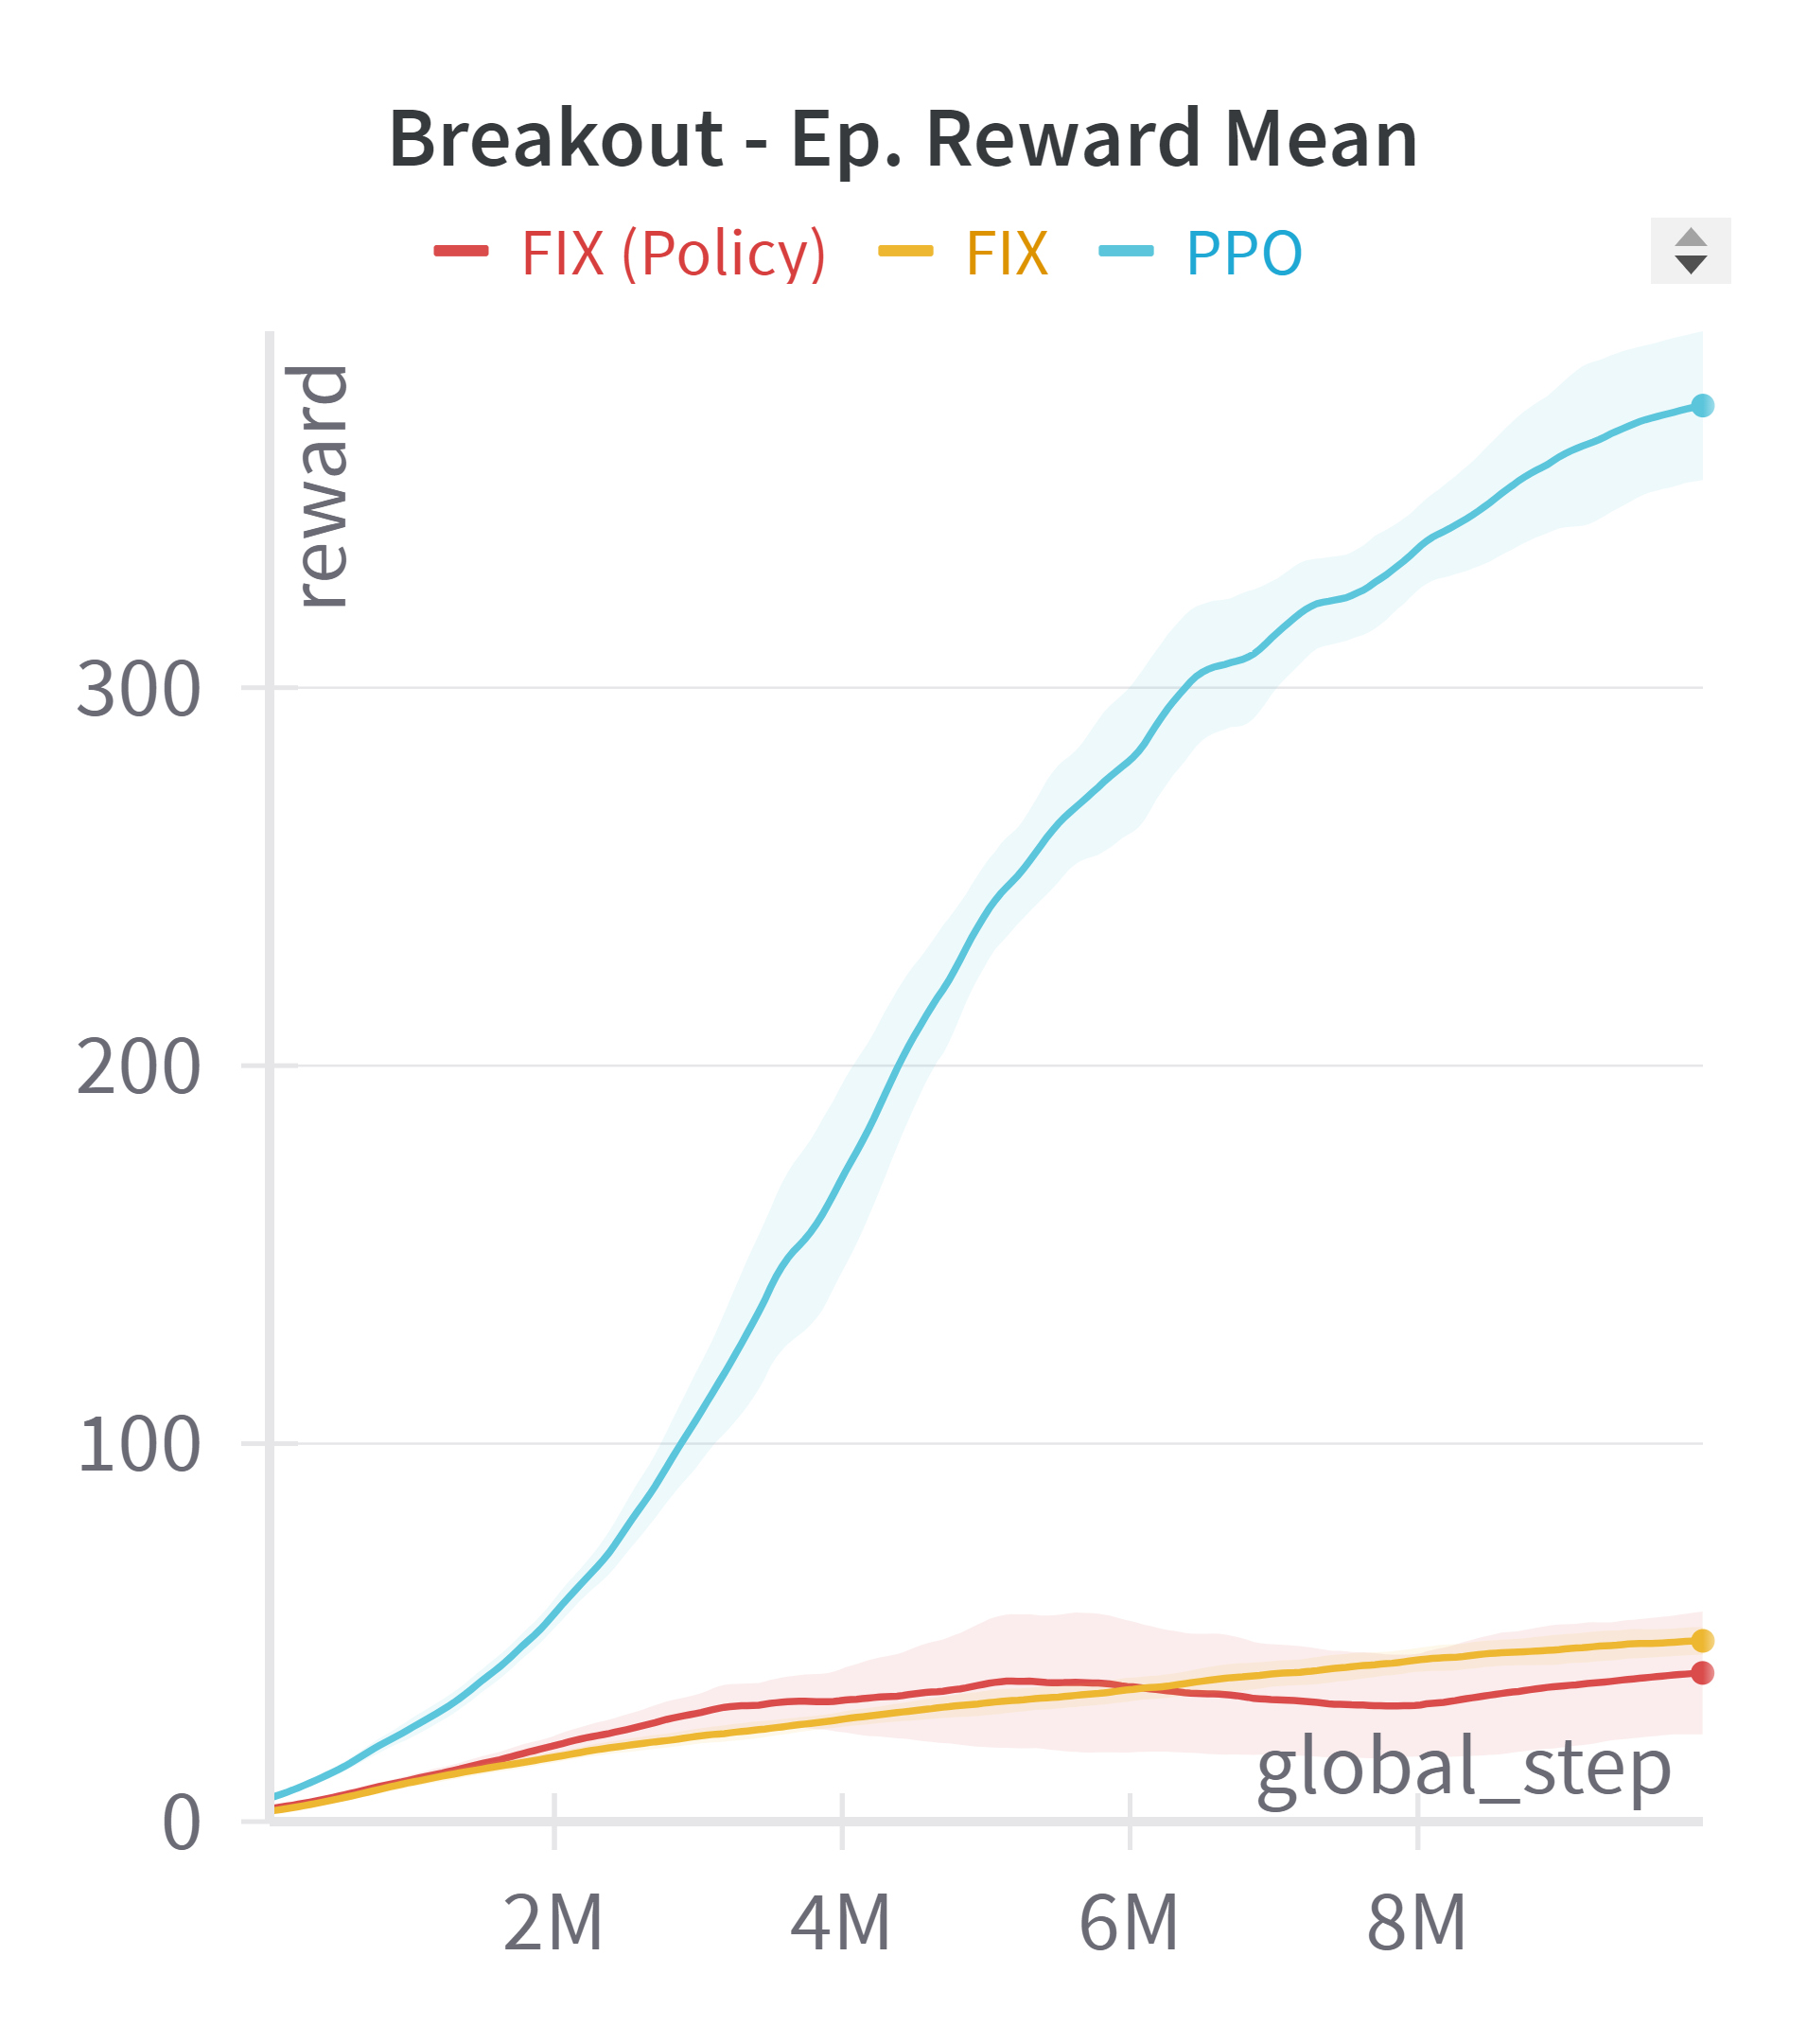
\includegraphics[width=\textwidth]{images/breakout_fix_policy}
        \label{fig:breakout_weights1}
    \end{subfigure}
    \hfill
    \begin{subfigure}[b]{0.45\textwidth}
        \centering
        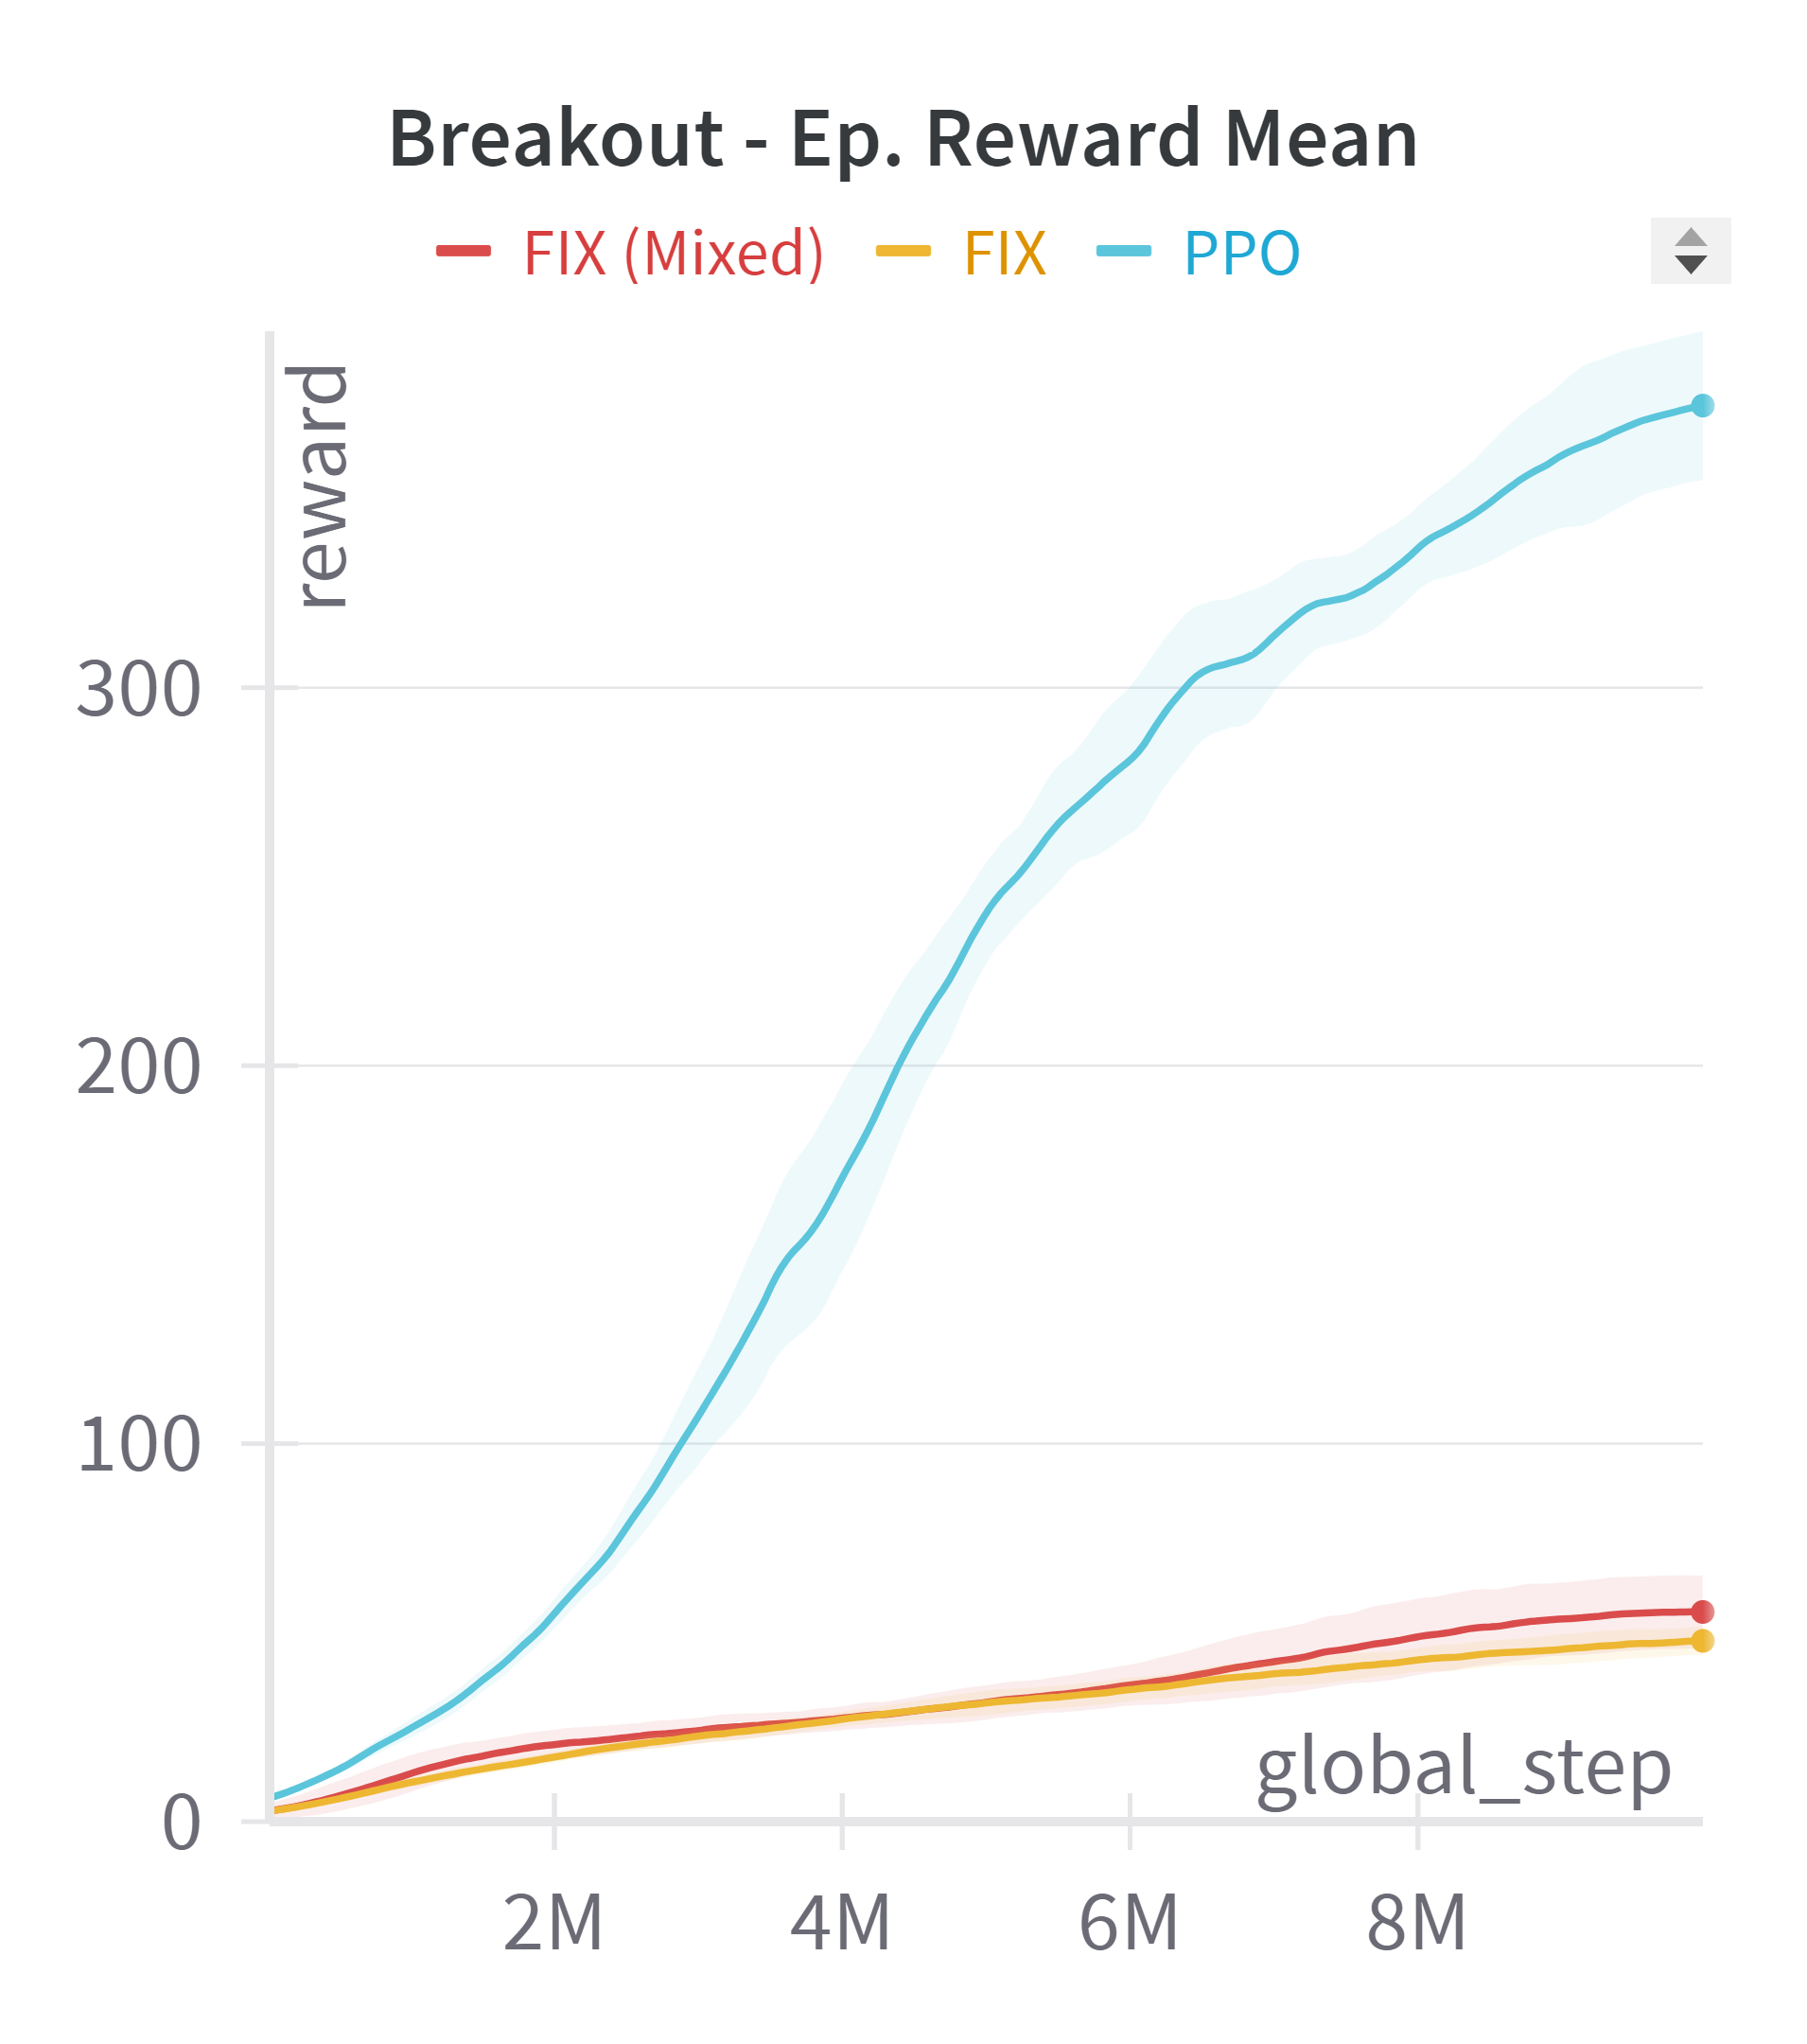
\includegraphics[width=\textwidth]{images/breakout_fix_mixed}
        \label{fig:breakout_weights2}
    \end{subfigure}

    \caption{TODO}
    \label{fig:breakout_attention}
\end{figure}


% STILL TO COMPLETE!!!!

%Lastly, Figure \ref{fig:inter} illustrates the enhanced \texttt{explainability} provided by WSA. By examining the current frames and the corresponding weights allocated by the shared component to each pre-trained model, one can appreciate agents' decision-making process. The visualization reveals how various FMs are leveraged in distinct contexts, shedding light on agents' dynamic adaptation of its prior knowledge.


%regarding pond and pacman



\section{Deep Q-Learning Experiments}\label{sec:dqn}

One last experiment is the one to prove that our approach is not limited to PPO algorithm, but is independent of the RL algorithm used.
To do so, we tested the effectiveness of the WSA module in combination with a Deep Q-learning agent.
As WSA is the main focus of our work, we decided to test only this module with different embedding sizes.
We did not test the other combination modules, this is to save computational resources and time since we already proved that combination modules are effective in RL, so we assume that they work also with DQL\@.
Using the same methodology and structure of experiments of the main work, we study the performance of the module.
We also restricted to test only the games of \textit{Breakout} and \textit{Ms. Pacman} as \textit{Pong} is very simple, and regarding \textit{Breakout} we FMs trained on the mixed dataset.

Figure~\ref{fig:dqn_experiments} shows that WSA works very well in comparison to the standard DQL agent, and the one with an embedding size of \texttt{256} results in the best performance.
In \textit{Ms. Pacman} the average cumulative reward is higher than DQL for all the training, meaning that the agent learns faster and better.
While in \textit{Breakout} it is faster to learn on the first part of the training, and at the end DQL results a little bit better.
This is a behavior similar to the one observed with PPO agents in Section~\ref{sec:breakout_study}.


\begin{figure}[htbp]
    \centering
    \begin{subfigure}[b]{0.45\textwidth}
        \centering
        %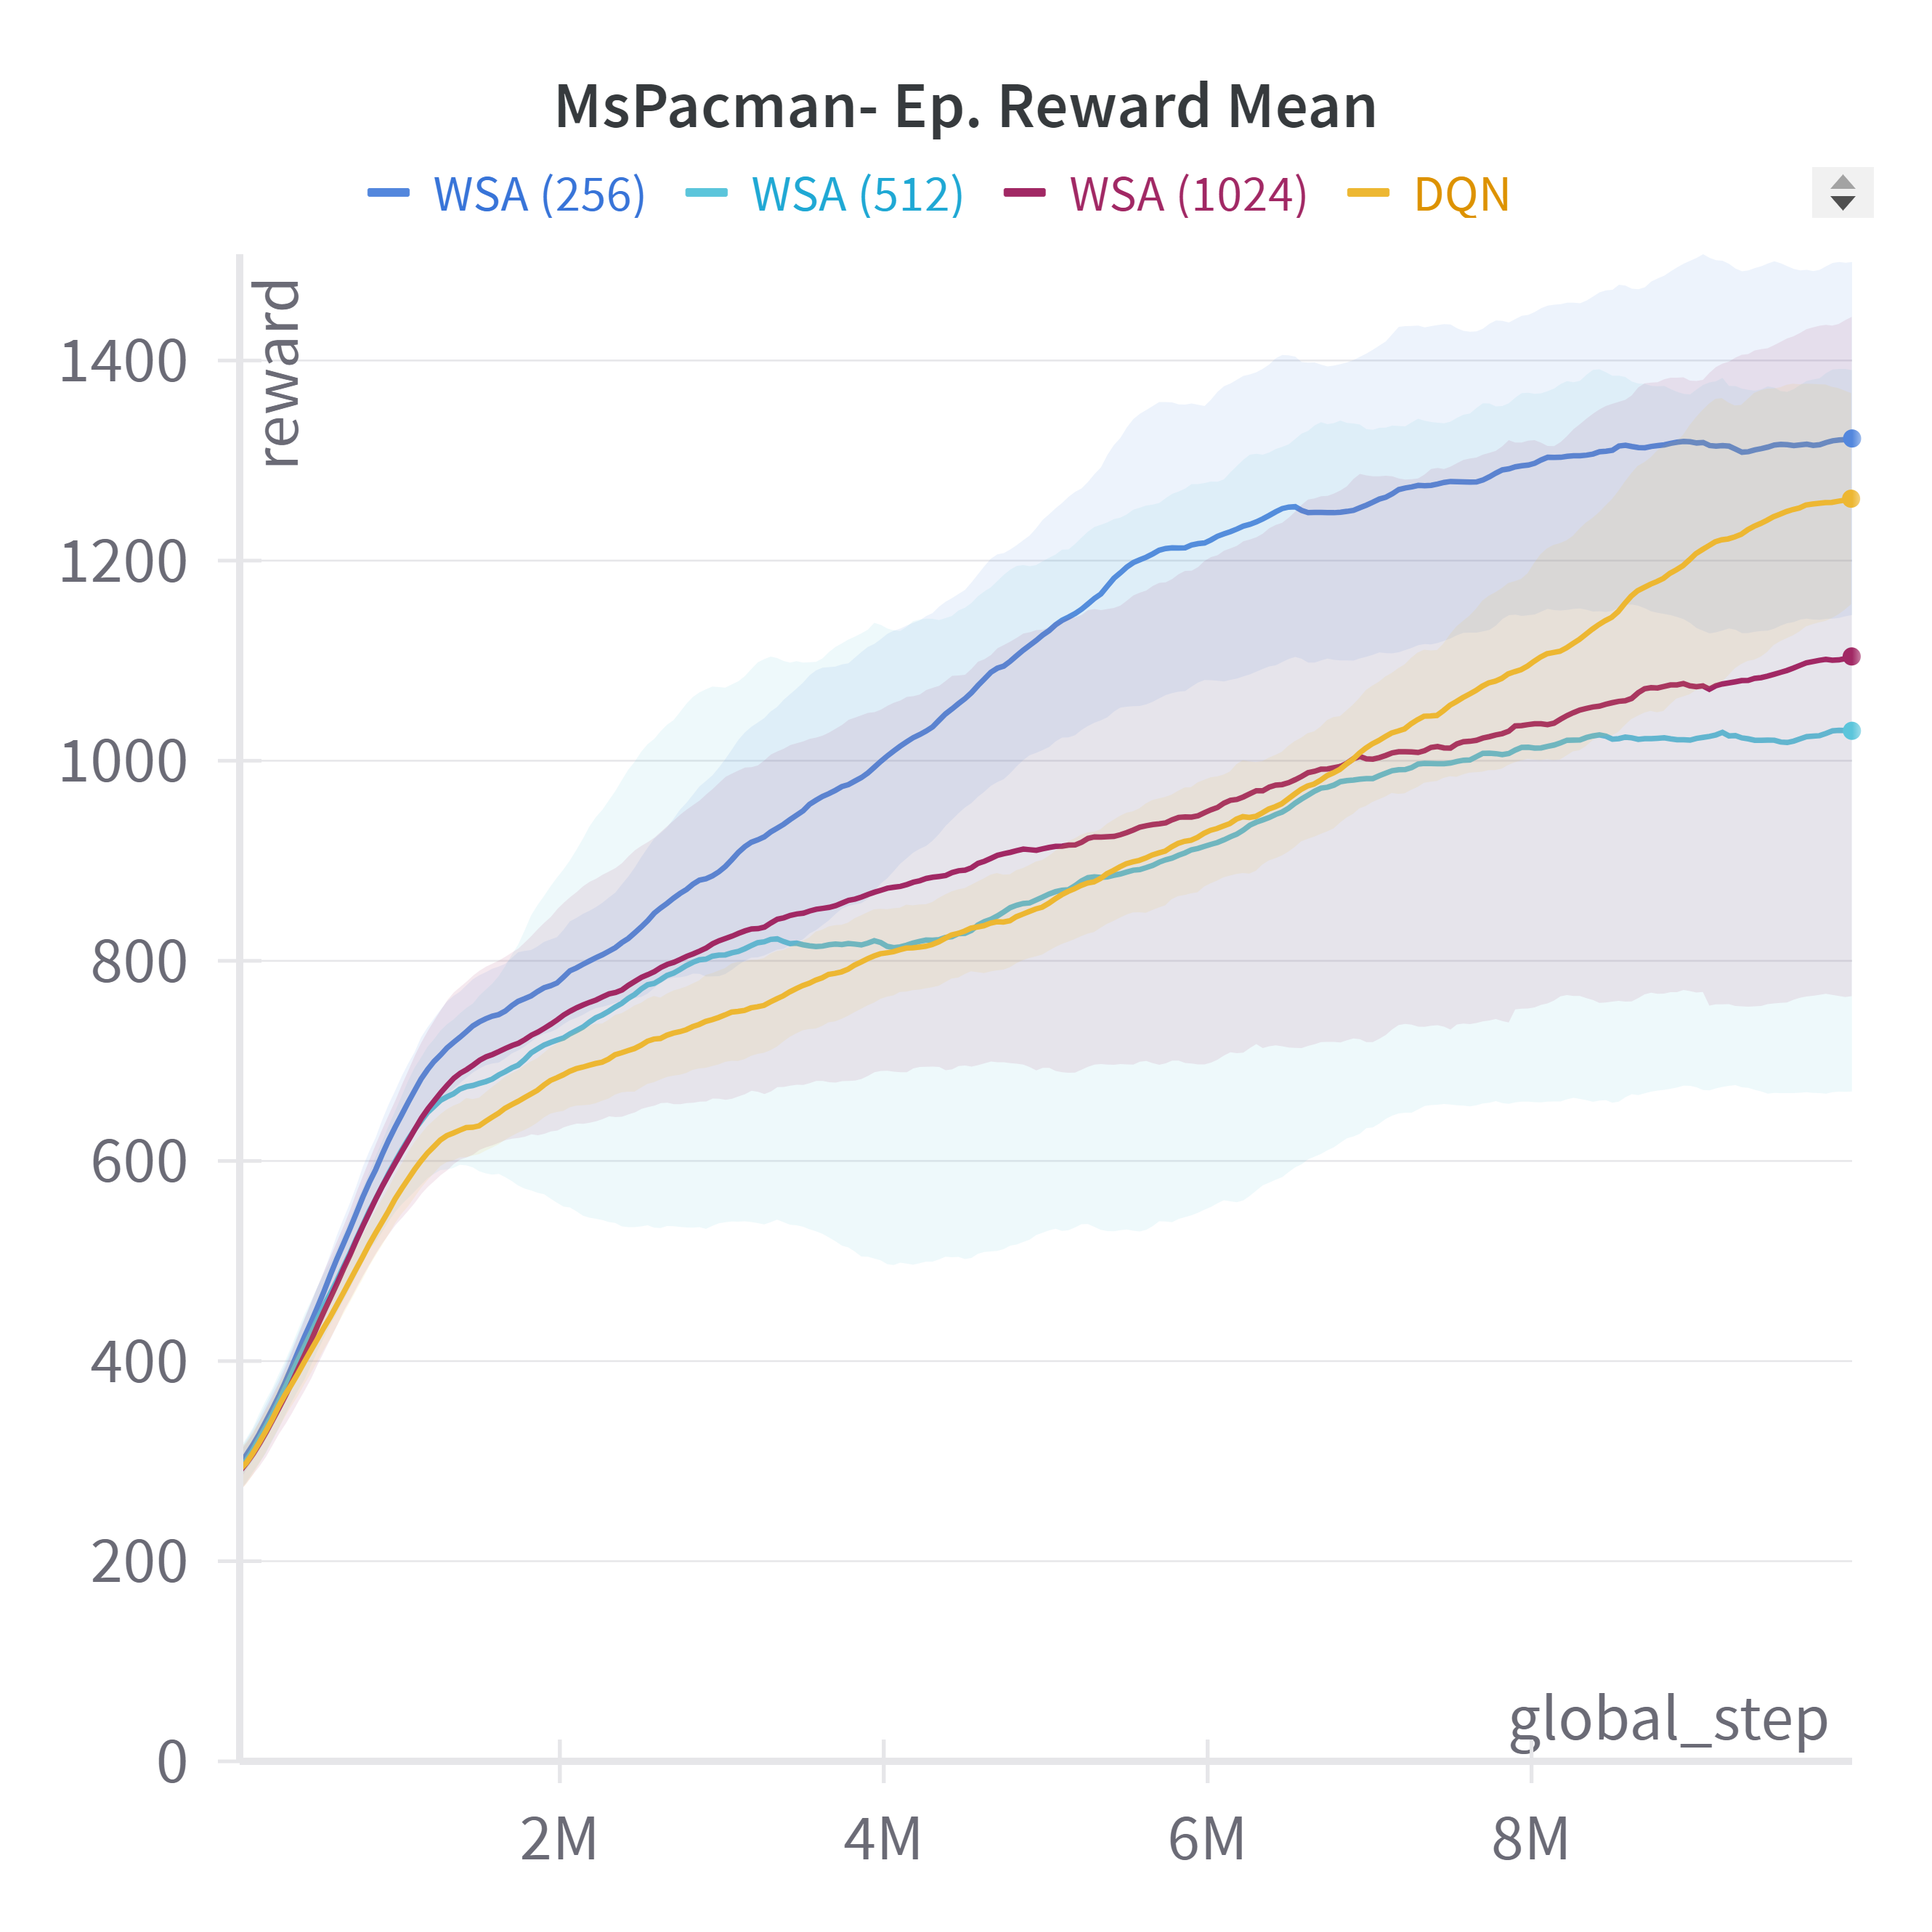
\includegraphics[width=\textwidth]{images/mspacman_dqn}
        \caption{\texttt{Ms. Pacman}}
        \label{fig:mspacman_dqn}
    \end{subfigure}
    \hfill
    \begin{subfigure}[b]{0.45\textwidth}
        \centering
        %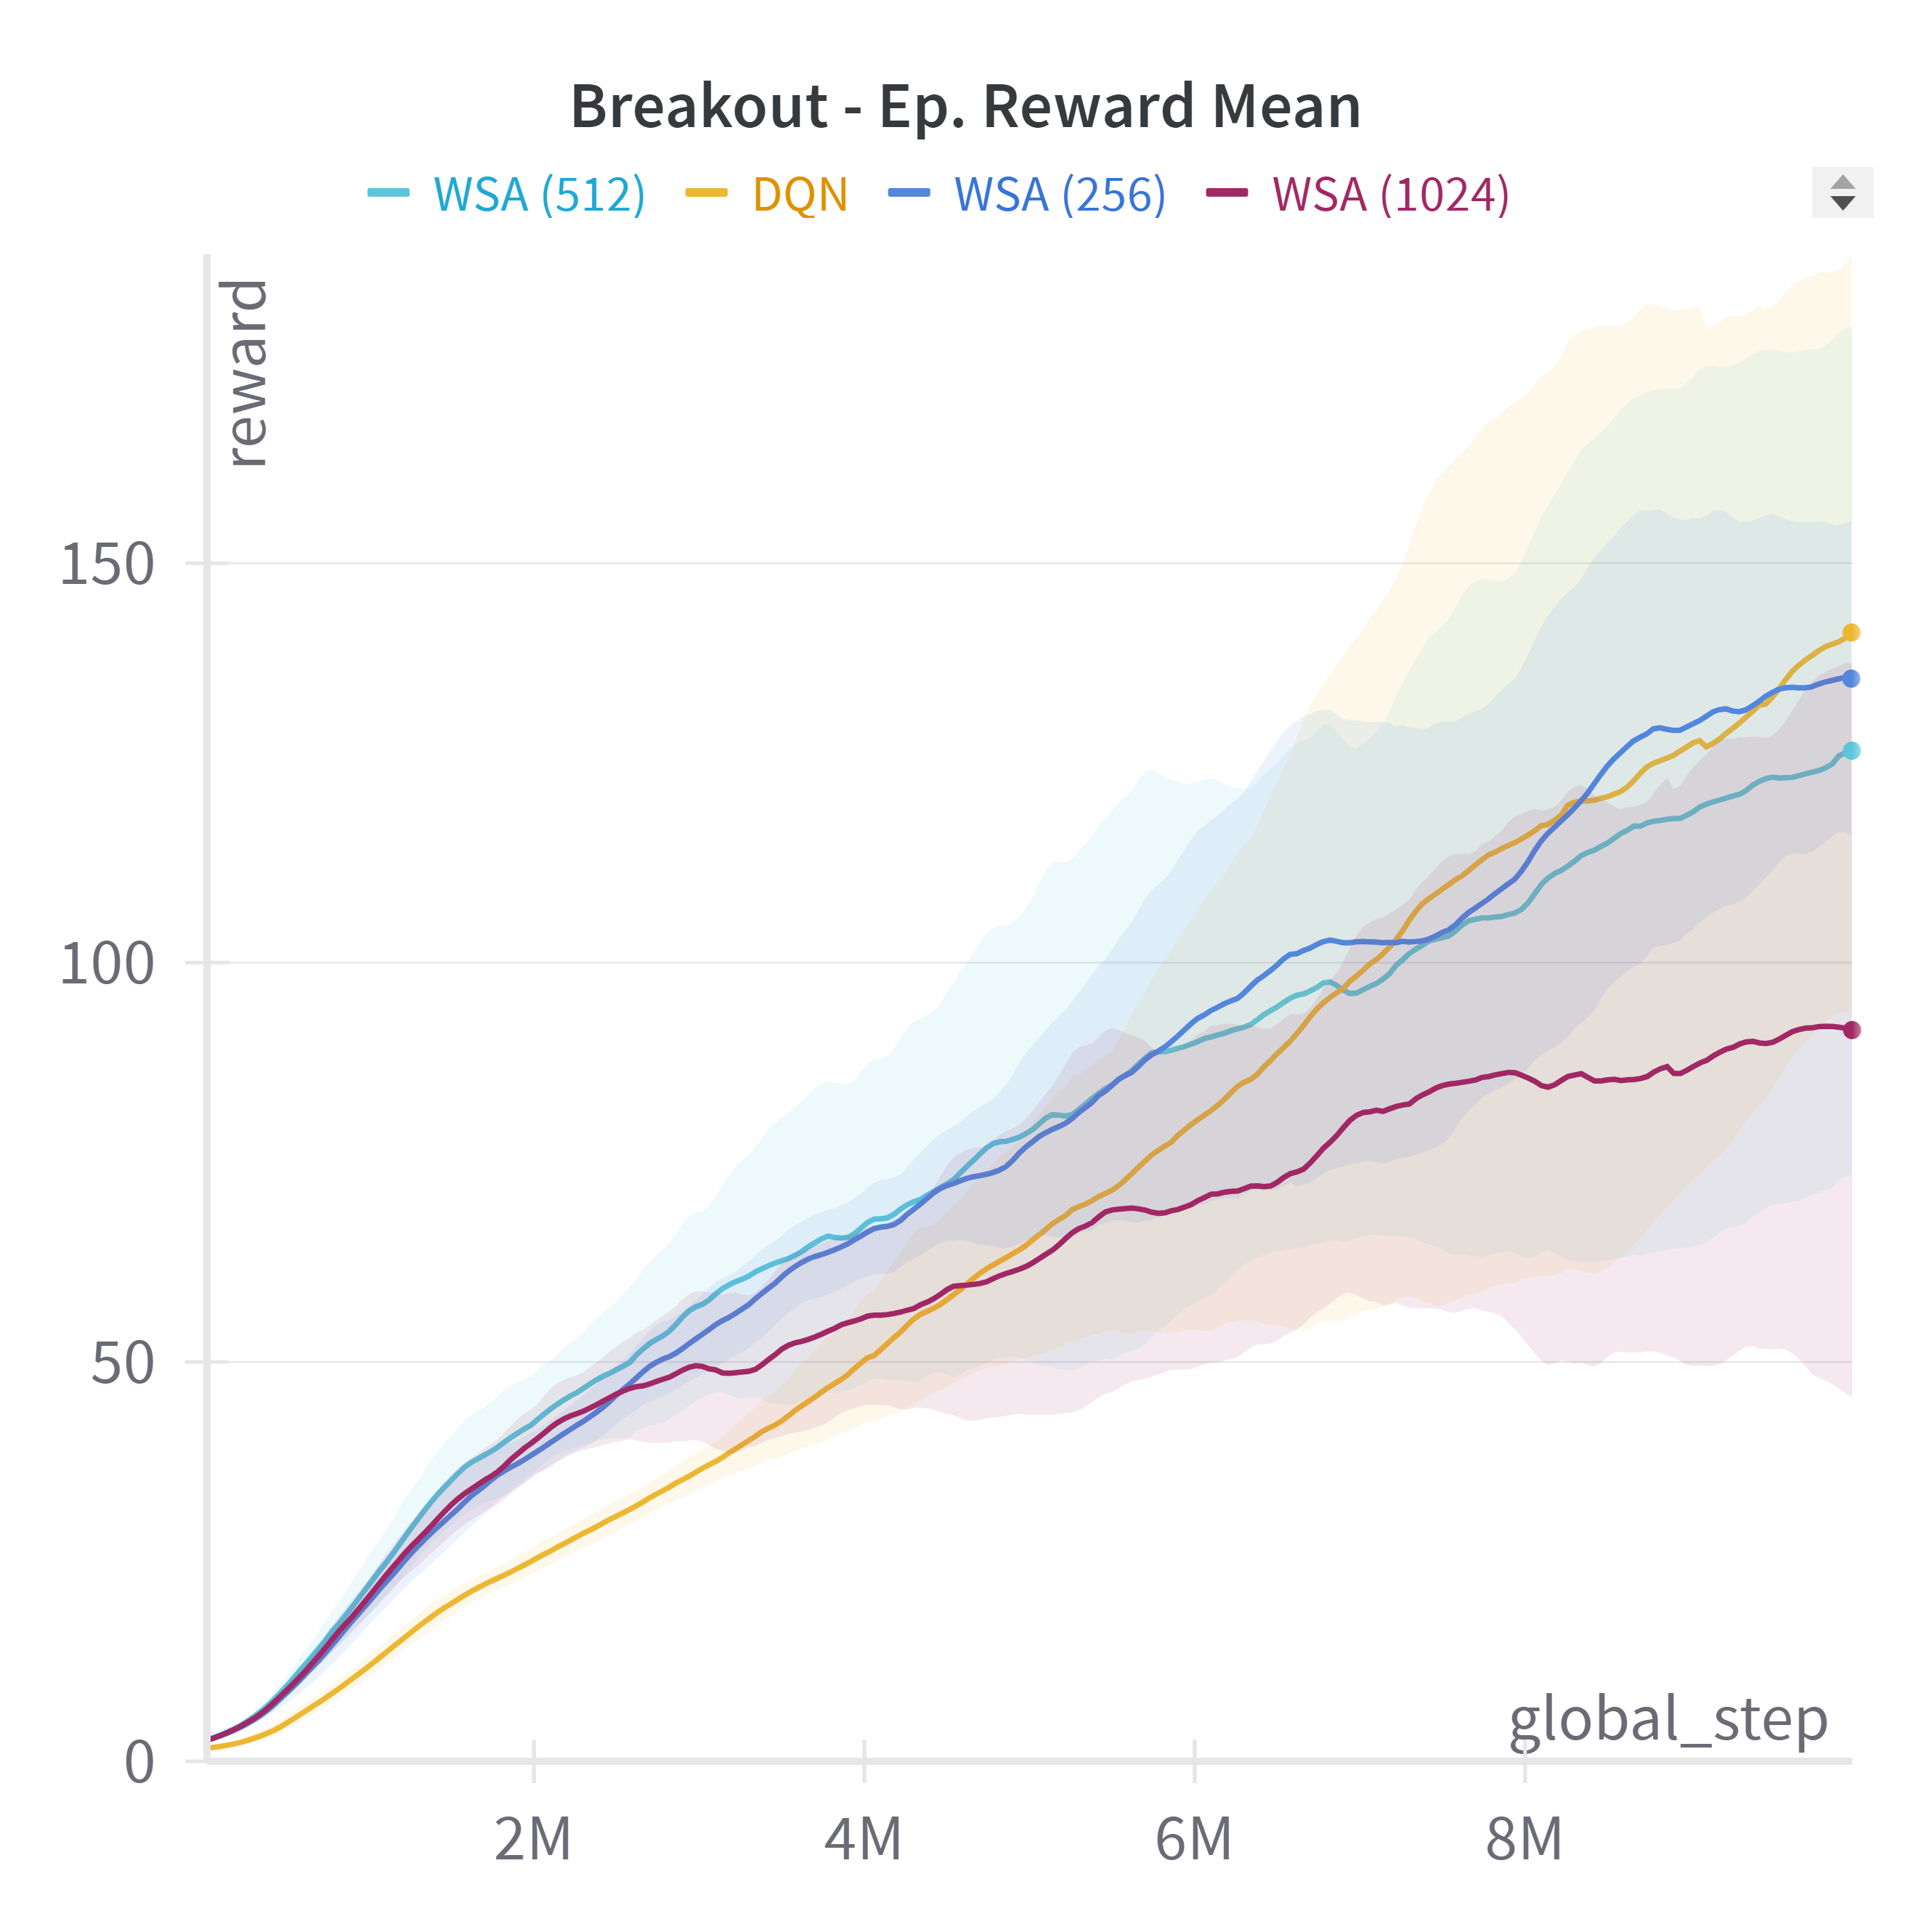
\includegraphics[width=\textwidth]{images/breakout_dqn}
        \caption{\texttt{Breakout}}
        \label{fig:breakout_dqn}
    \end{subfigure}
    \caption{Cumulative reward during training of different agents, comparing WSA and DQN. Each subfigure shows the mean score, with shaded areas indicating the standard deviations, across multiple agents.}
    \label{fig:dqn_experiments}
\end{figure}



We selected for evaluation the agent with \texttt{256} as embedding size since it is the best performing during training.
This time to evaluate the agents, instead of selecting the best model between the \texttt{4} runs during training, we tested all the models across \texttt{5} random seeds for \texttt{50} episodes.
Table~\ref{tab:dqn_results} reports the averaged results during evaluation.
We notice how WSA results in a higher score in both games and in particular in \textit{Breakout} the agent scores \texttt{213} compared to \texttt{166} of DQL\@.
Please note that PPO agents reached a higher score in \textit{Breakout} and these results are not directly comparable as the two algorithms have different learning dynamics and different ways to interact with the environment.
Lastly, we can conclude that WSA works well regardless of the RL algorithm used, and it can be a valuable tool to improve the performance of agents in different scenarios.



\begin{table}[ht]
    \begin{center}
        \begin{tabular}{lll}
            \multicolumn{1}{l}{Environment}  &\multicolumn{1}{l}{\textbf{Agent}} &\multicolumn{1}{l}{\textbf{Reward}}
            \\ \hline \\

            \multirow{2}{*}{\texttt{Ms. Pacman}}
                                  & \textbf{WSA} & \textbf{2047.27 $\pm$ 231.18} \\
                                  & DQL & 1701.00 $\pm$ 490.41 \\
                                  \\ \hline \\

            \multirow{2}{*}{\texttt{Breakout}}
                                  & \textbf{WSA} & \textbf{213.14 $\pm$ 39.37} \\
                                  & DQL & 166.65 $\pm$ 20.19 \\

        \end{tabular}
    \end{center}
    \caption{Performance during evaluation averaged across 5 different seeds, using WSA with the embedding size of 256.}
    \label{tab:dqn_results}
\end{table}



\section{Final considerations}\label{sec:final-considerations}
In this Section, we want to provide some final considerations about our work.
We have shown that our approach is effective in improving the performance of agents in different scenarios, and it can be applied to different RL algorithms.
Also, we have shown how the quality of the training data is crucial for the performance of the agent and how WSA can provide explainability to the decision-making process of the agent.
But there are still some considerations that need to be addressed.

First of all, the computational cost of our approach.
Using pre-trained models can be computationally expensive, and it can be a bottleneck in the training process.
In fact, compared to an end-to-end solution, our approach is able to process more or less half of the frames per second. \footnote{The training time is measured considered a shared server and can be influenced by other processes running on the machine.}
This is due to the fact that, even if the pre-trained model weights are frozen during training, they need to process the frames before the agent can make a decision.
As the number of FMs increases, the computational cost increases, and the agent needs to wait more time to make a decision.
In our implementation, the frames are processed sequentially, and the agent needs to wait for all the FMs to provide their representation before making a decision.
This can be a problem in real-time applications, where the agent needs to make decisions in a short amount of time.
A possible solution to this problem could be to process the frames in parallel, and to make the agent wait only for the slowest FM to provide its representation.

Another consideration is in the number of trainable parameters of the whole model.
Different combination modules have different numbers of parameters, and may result in different computational costs.
Table~\ref{tab:parameters} shows the number of parameters of the different combination modules compared to an end-to-end PPO.
We notice that we considered only the models with \textit{Fully-Connected Network} of \texttt{256} units.

\begin{table}[ht]
    \begin{center}
        \begin{tabular}{ll}
            \multicolumn{1}{l}{\textbf{Feature Extractor}}  &\multicolumn{1}{l}{\textbf{Parameters}}
            \\ \hline \\
            LIN              &  \texttt{8.7M} \\
            FIX        & \texttt{4.9M}--\texttt{19.4M} \\
            CNN       & \texttt{4.2M}\\ % the number of parameters did not increased so much
            MIX       & \texttt{4.5M} \\
            RES           & \texttt{0.3M}--\texttt{1.1M} \\
            DPA             & \texttt{8.7M}--\texttt{34.7M} \\
            WSA         & \texttt{8.7M}--\texttt{34.7M} \\
            PPO             & \texttt{1.6M} \\

        \end{tabular}
    \end{center}
    \caption{The table shows the number of parameters of the whole model from the little configuration to the biggest.}
    \label{tab:parameters}
\end{table}

%Write some conclusions

%%! Author = giaco
%! Date = 12/06/2024

\chapter{Results}
\label{sec:results}

\subsection{Main Results}\label{sec:results_1}
In the following empirical evaluation, we used the same methodology and setup adopted for initial experiments. For each game, multiple agents instances are trained using different seeds. For a comprehensive view of agents' performance, the behavior is averaged over different versions. Figure \ref{fig:trainresults} shows the average learning curves of agents during training - the shaded area depicts the standard deviation. To ensure robust evaluation, agents are tested across \texttt{5 random seeds} for \texttt{50 episodes}, specifically: 47695, 32558, 94088, 71782 and 66638. Table \ref{tab:results} reports the averaged results during evaluation of the best agent during training. We address the elephant in the room - Figure \ref{fig:breakouttrain} - in the next section \ref{sec:breakout_study}.

\begin{figure}[ht]
    \centering
    \begin{subfigure}[b]{0.32\textwidth}
        \centering
        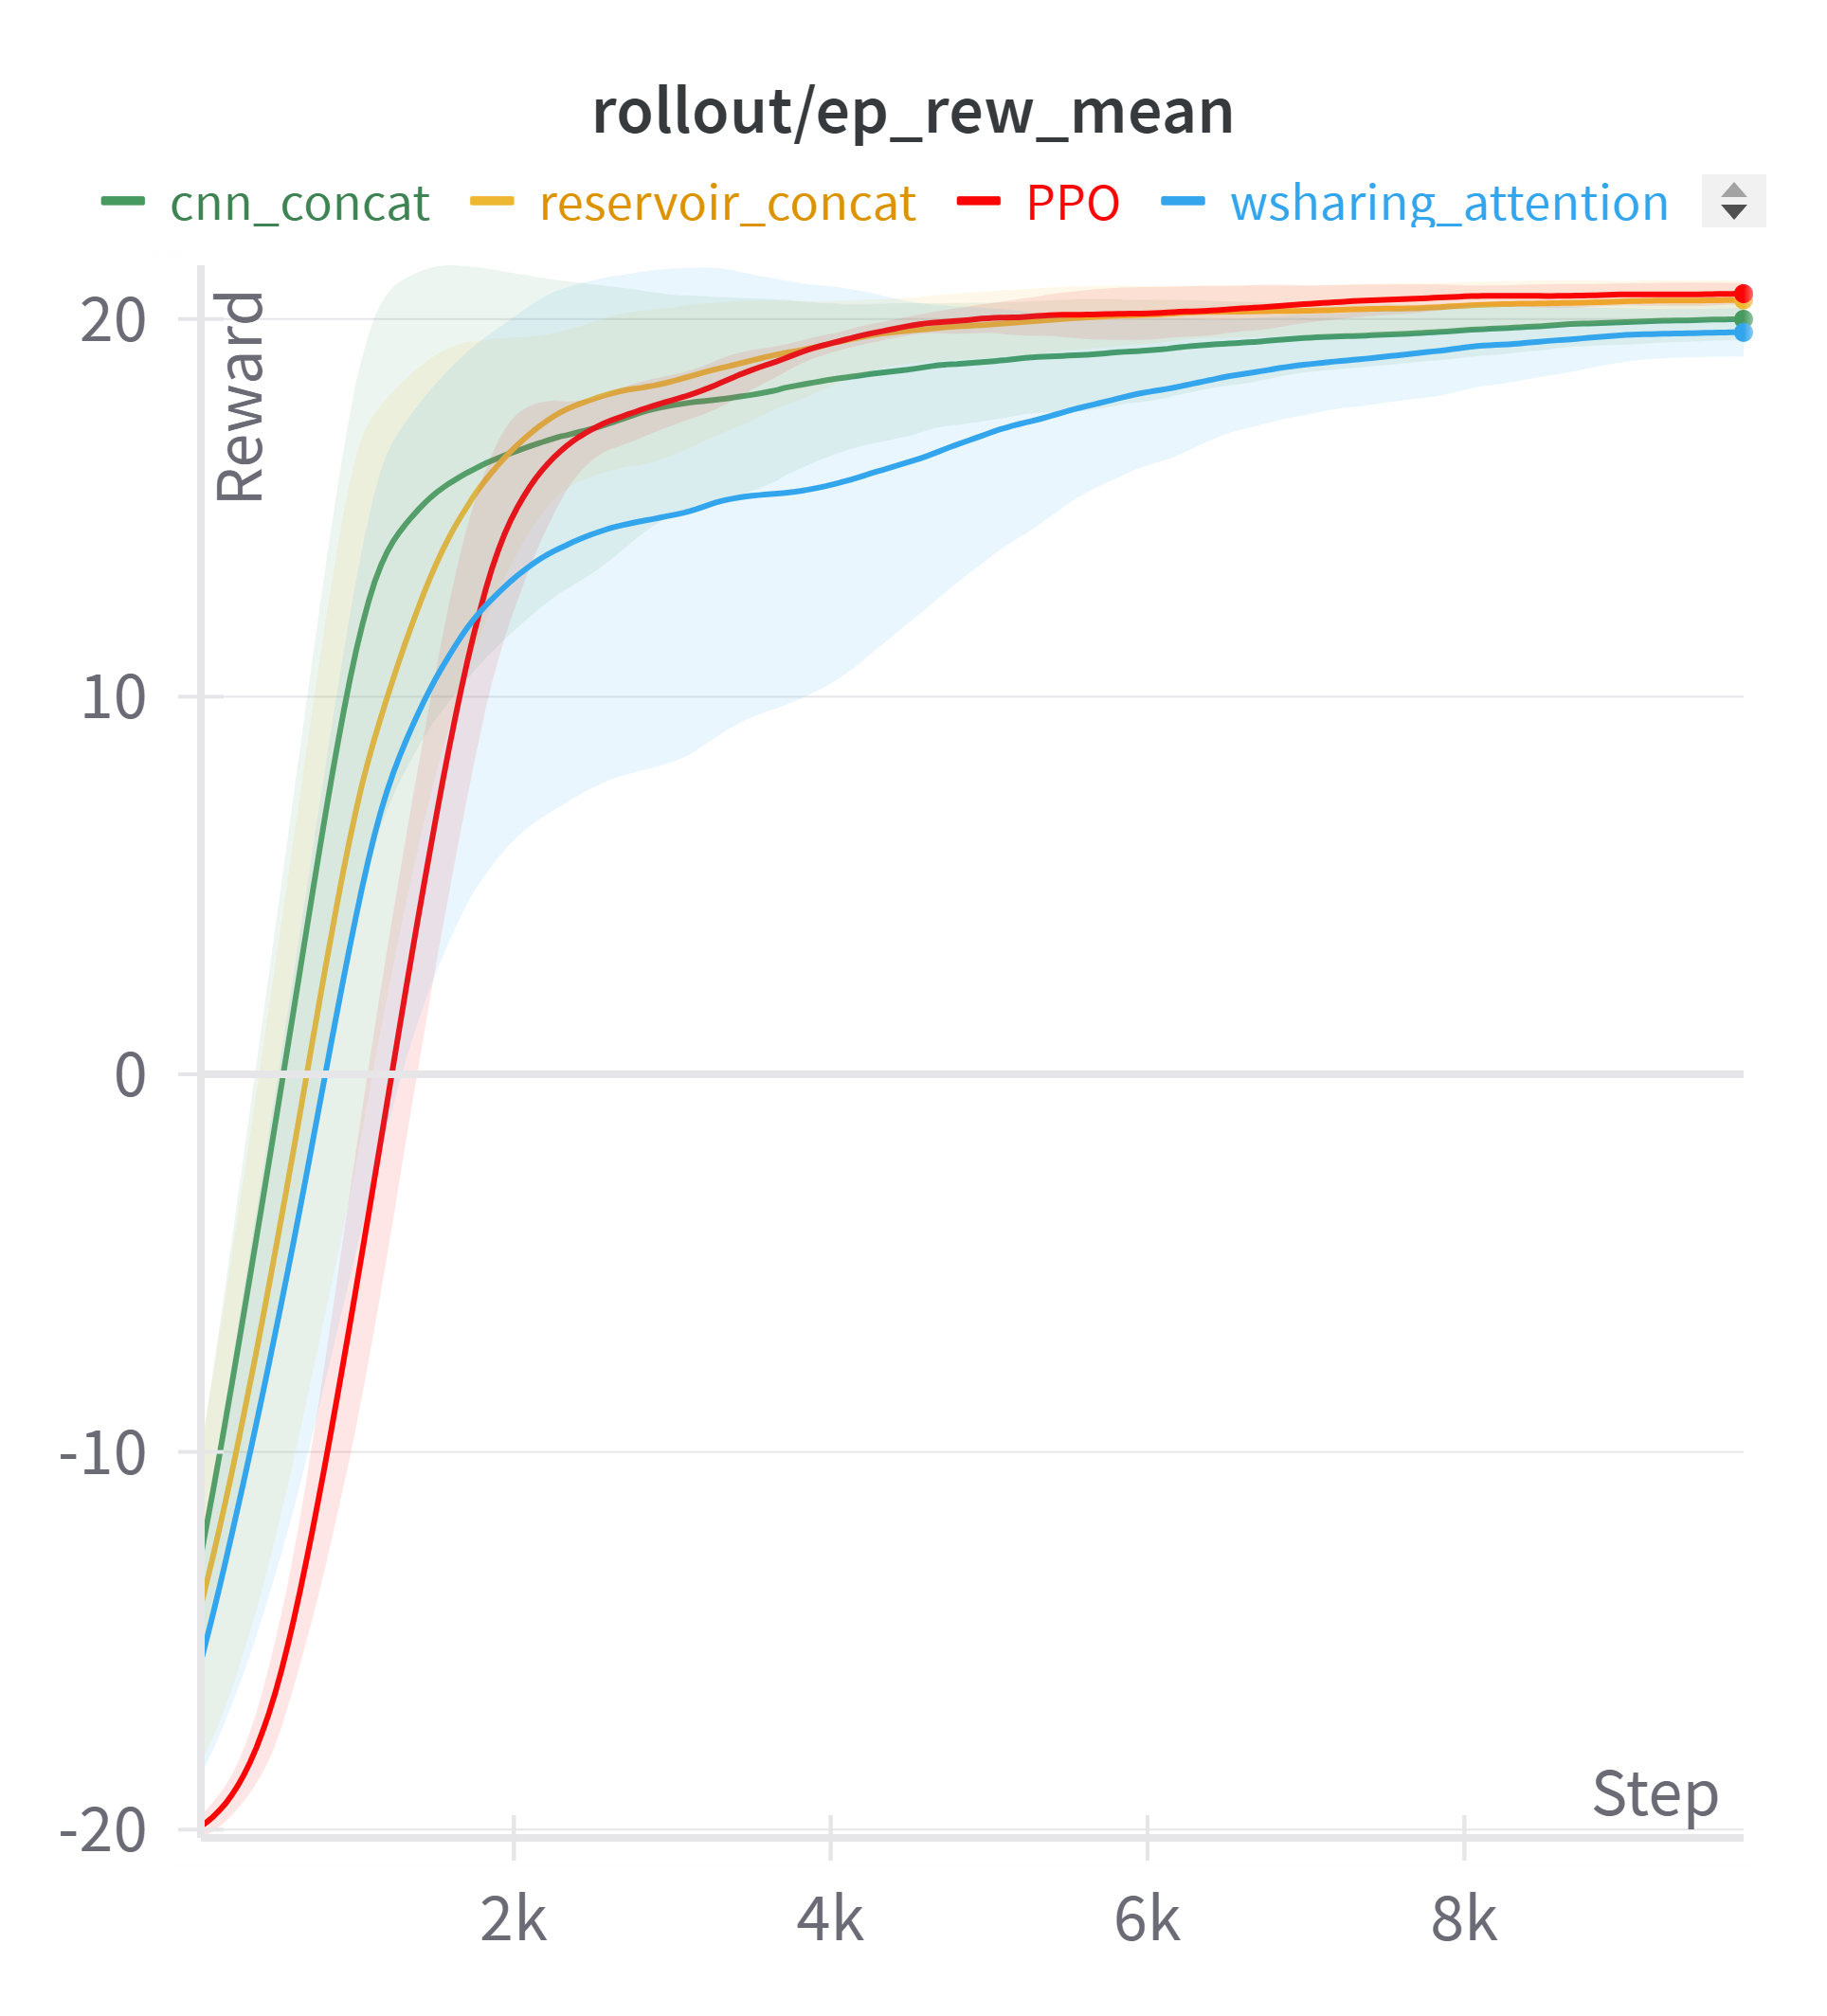
\includegraphics[width=\textwidth]{images/pong_train.png}
        \caption{\texttt{Pong}}
        \label{fig:pongtraining}
    \end{subfigure}
    \hfill
    \begin{subfigure}[b]{0.32\textwidth}
        \centering
        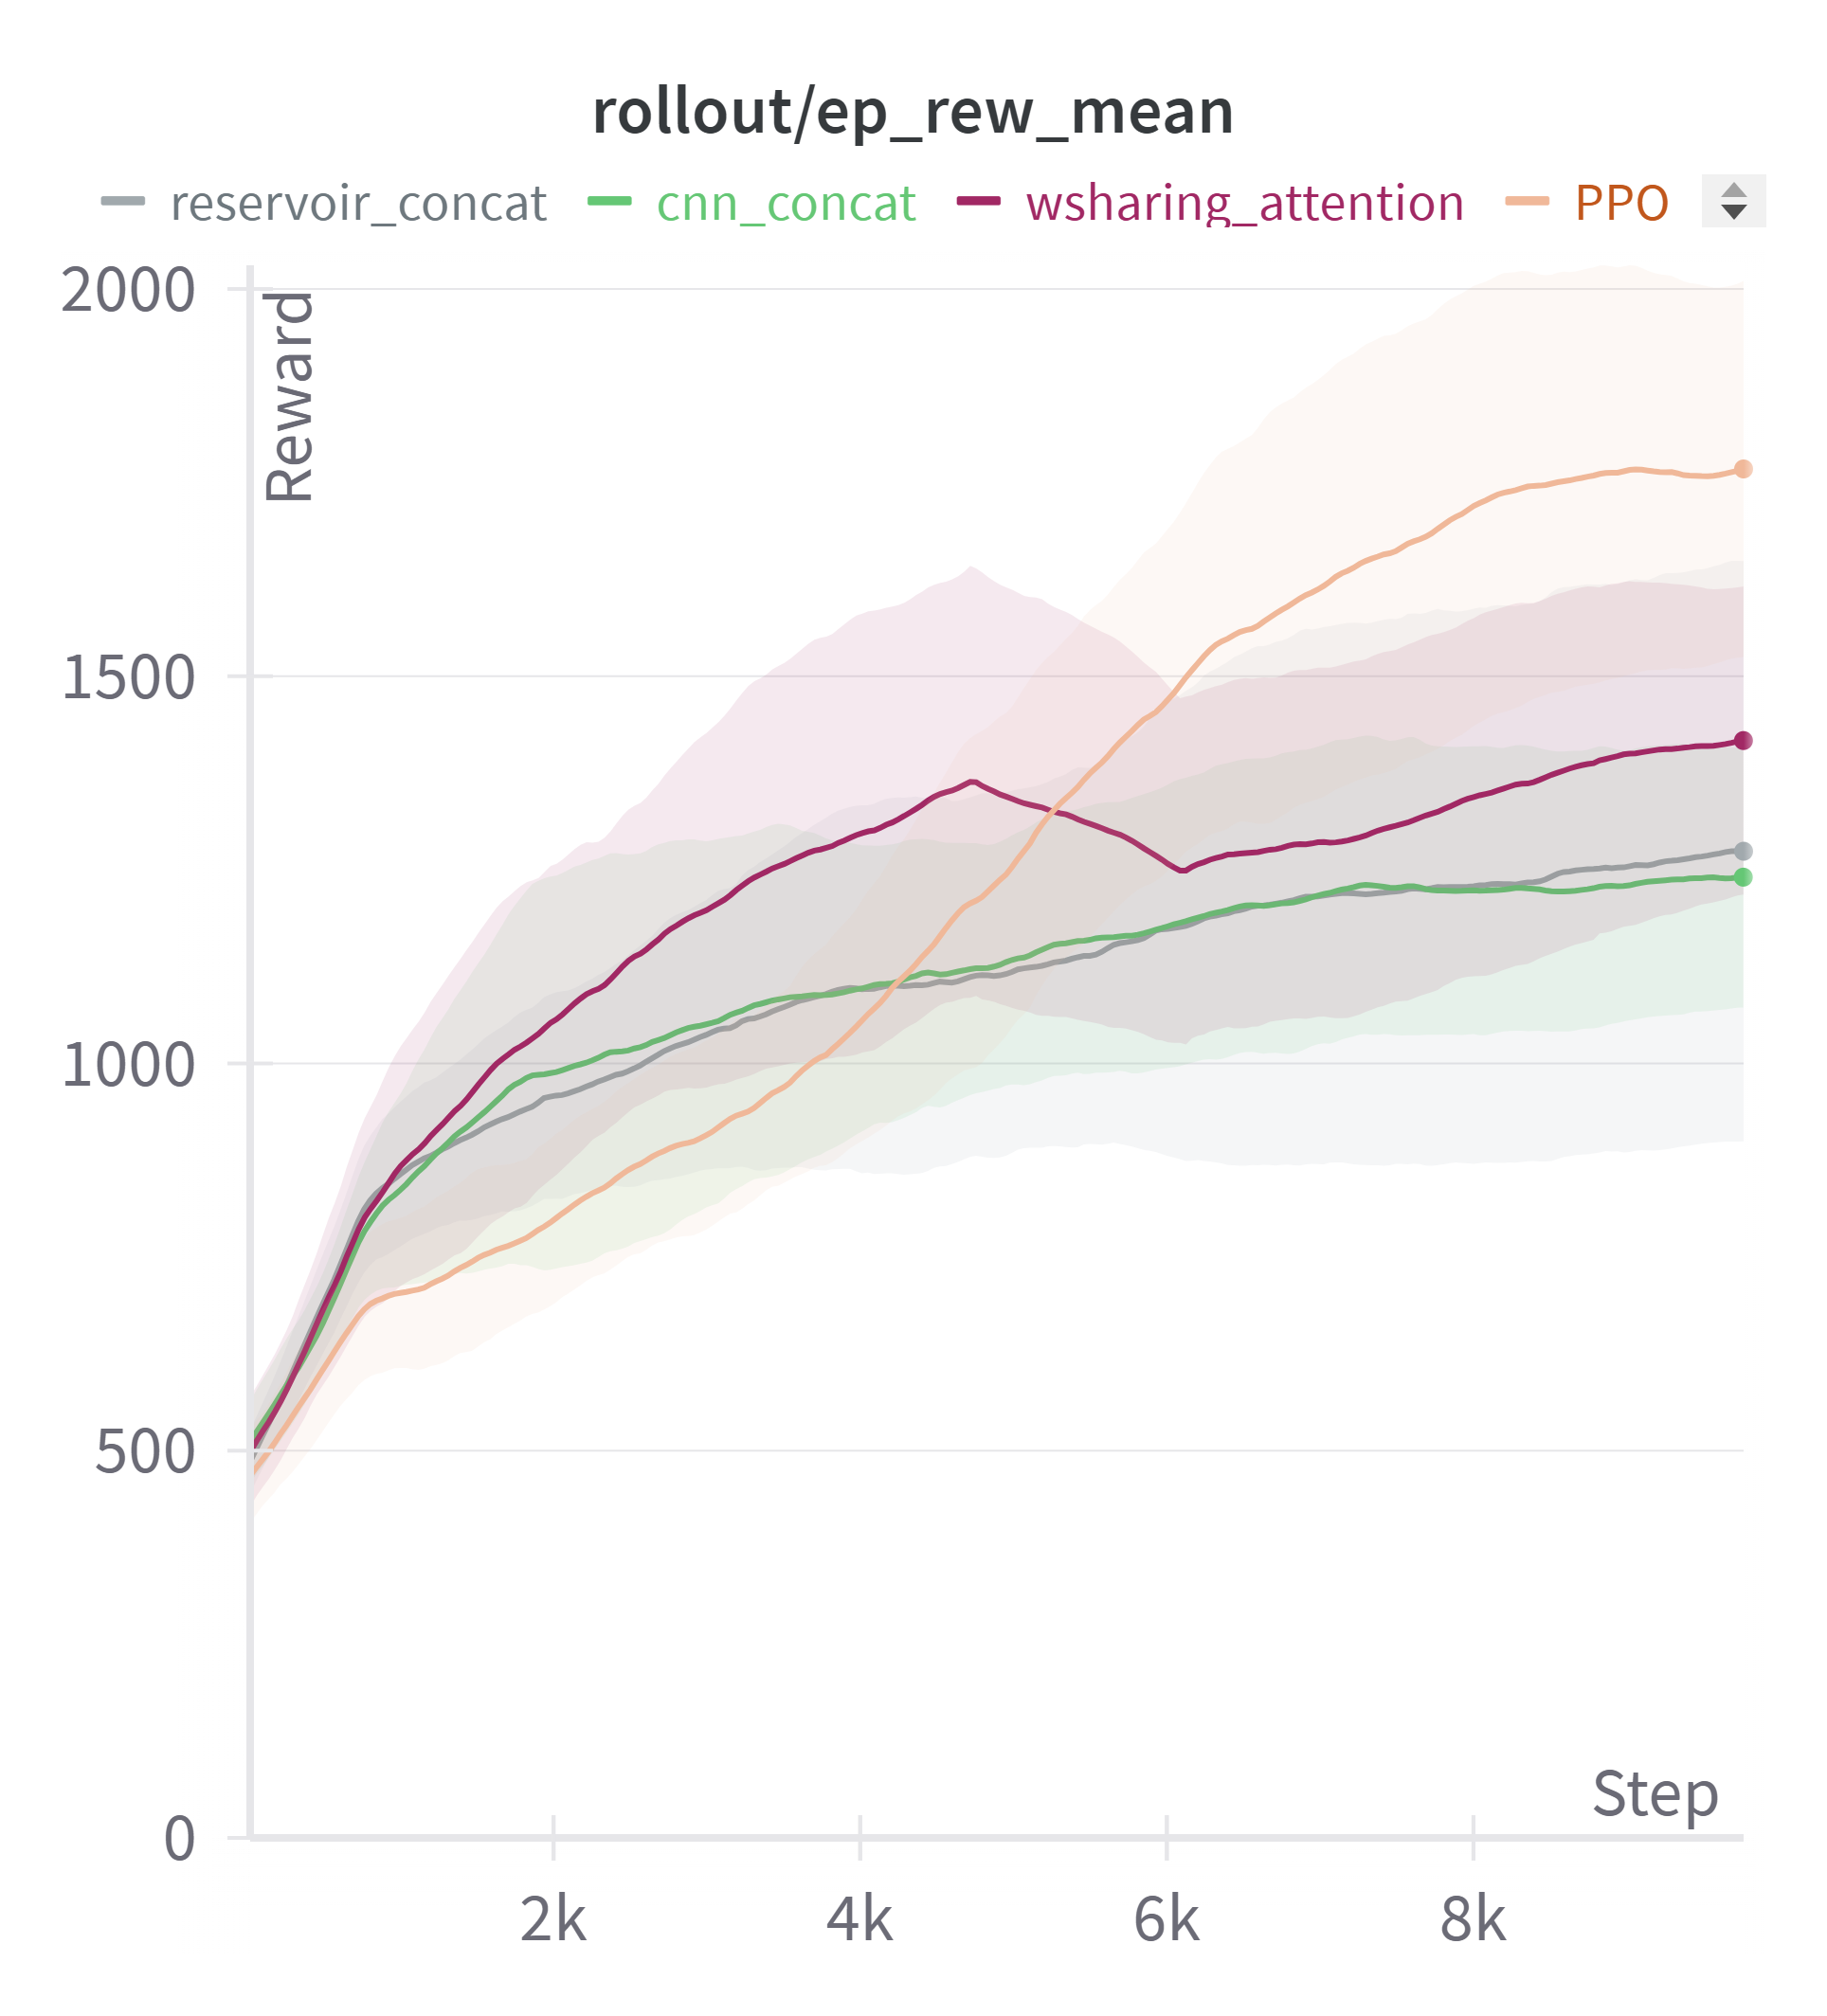
\includegraphics[width=\textwidth]{images/mspacman_train.png}
        \caption{\texttt{Ms.Pacman}}
        \label{fig:mspacmantrain}
    \end{subfigure}
    \hfill
    \begin{subfigure}[b]{0.32\textwidth}
        \centering
        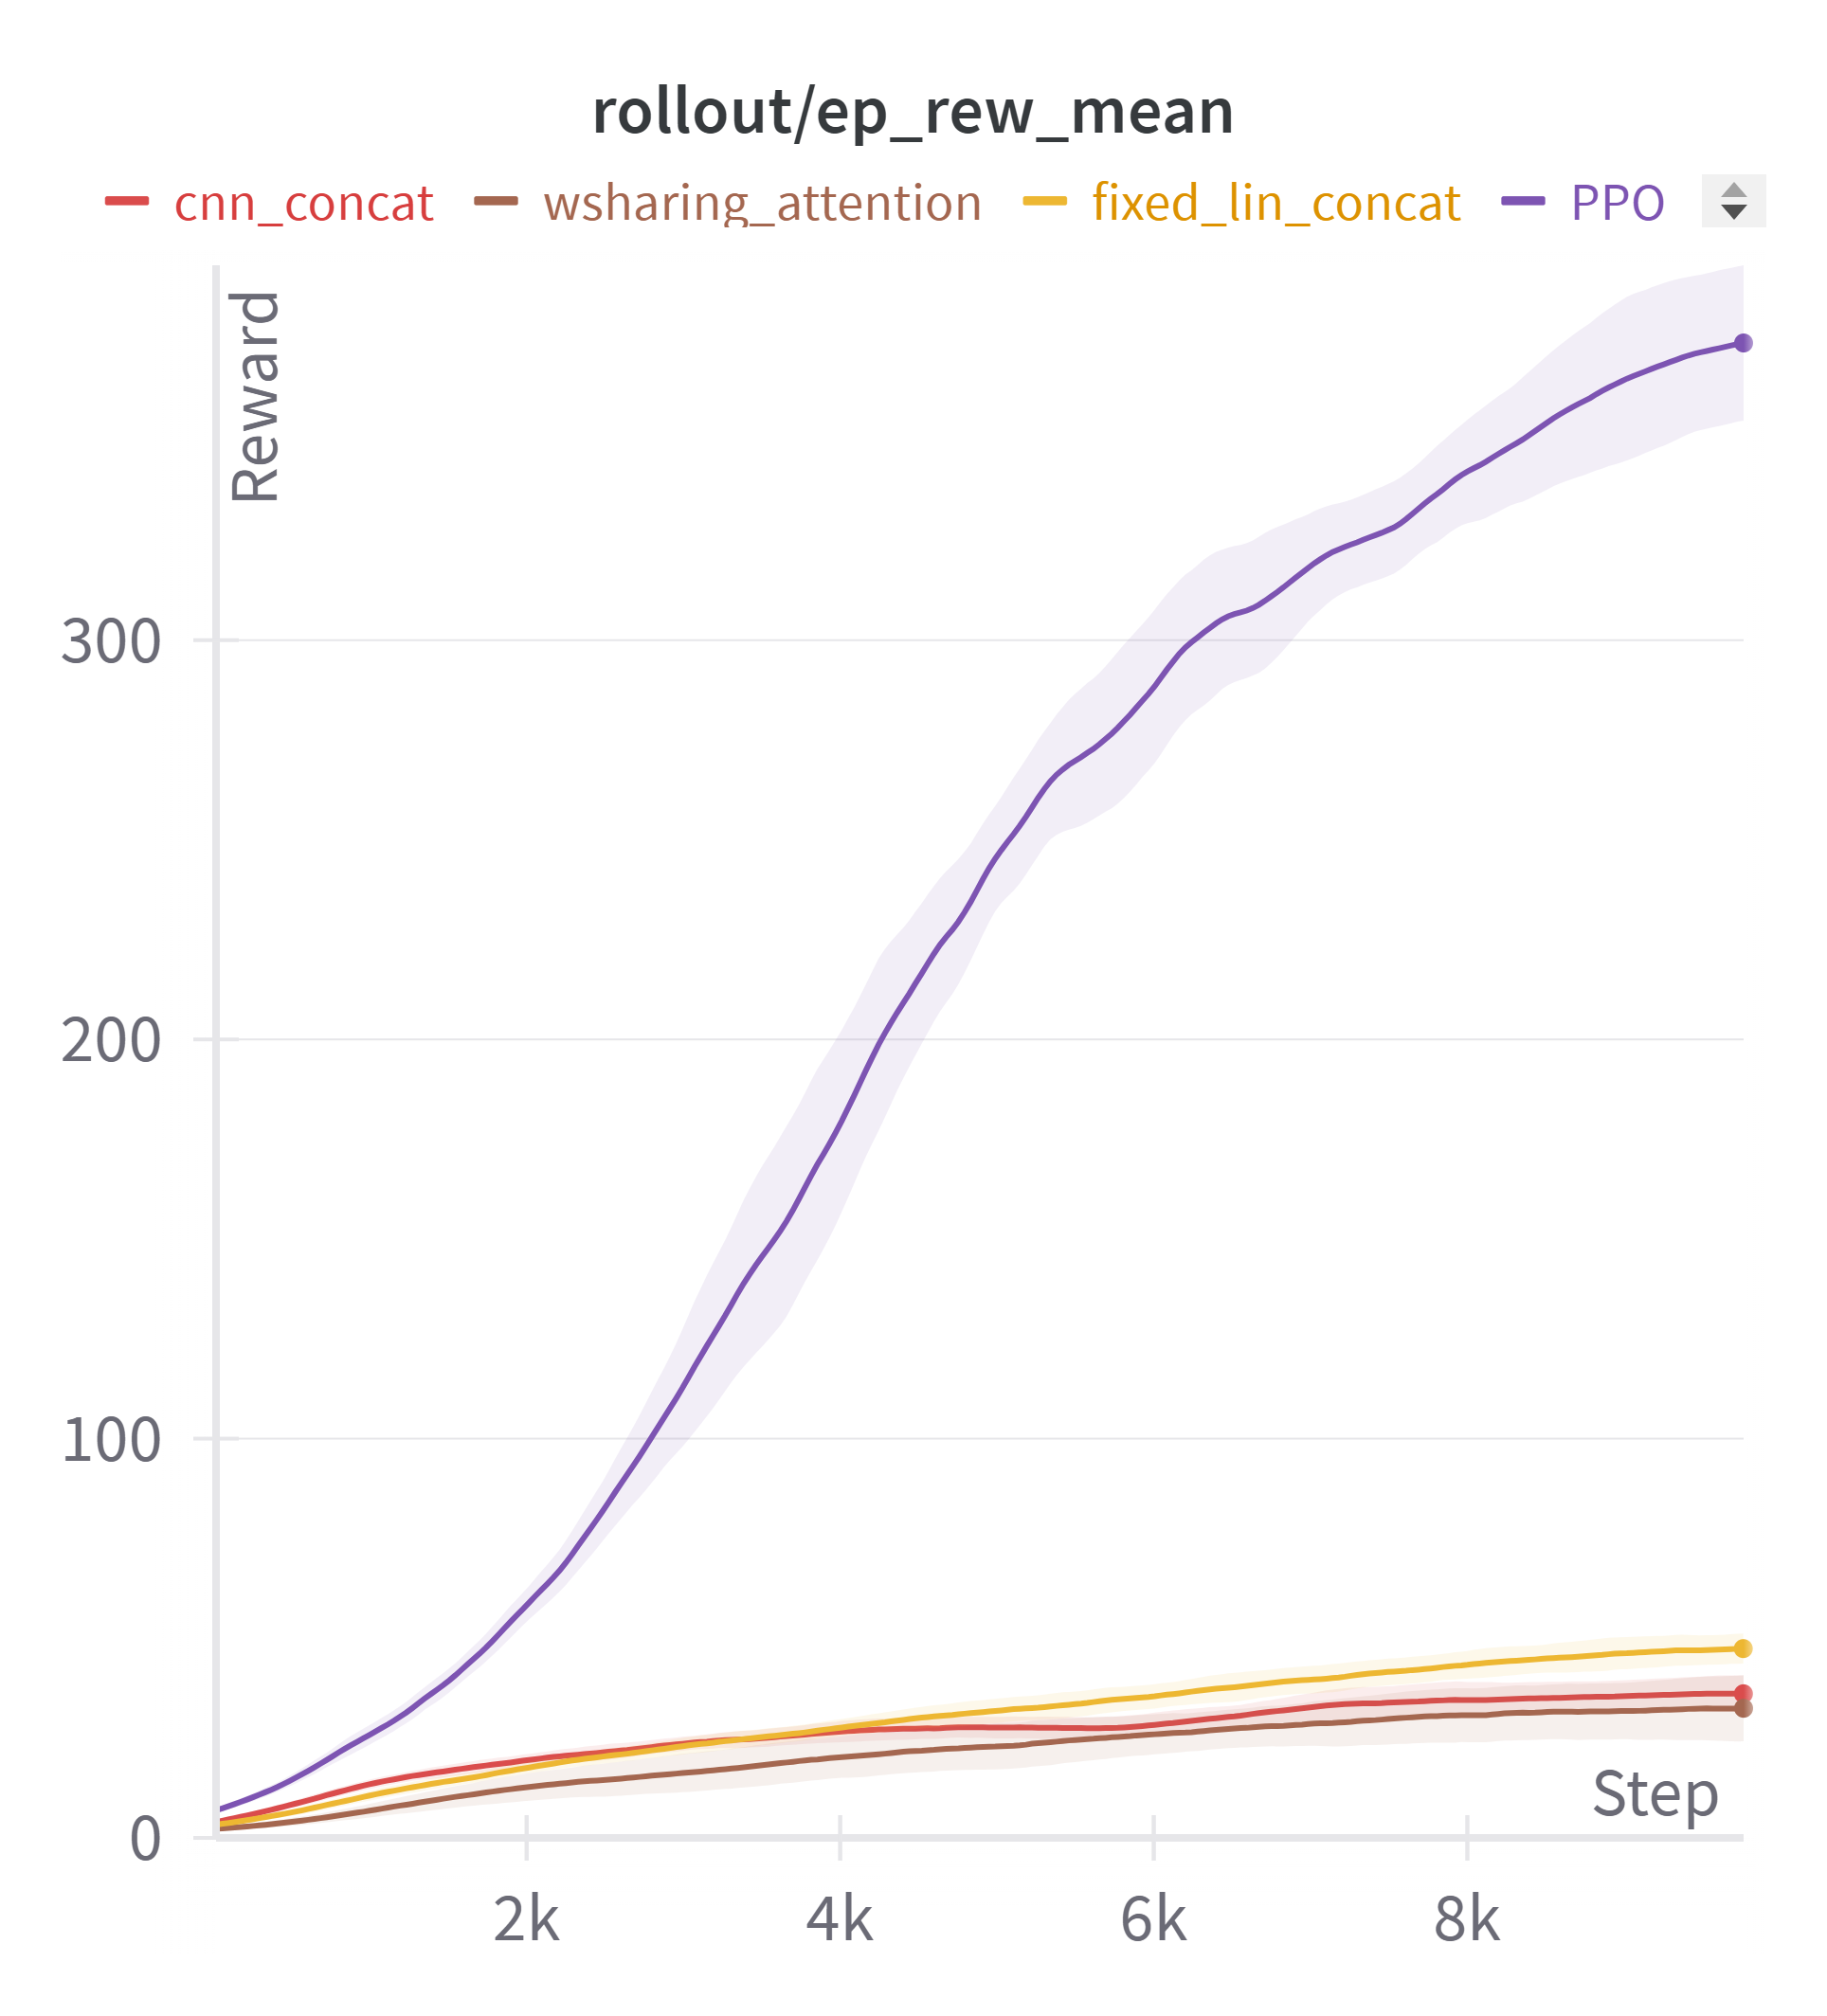
\includegraphics[width=\textwidth]{images/breakout_train.png}
        \caption{\texttt{Breakout}}
        \label{fig:breakouttrain}
    \end{subfigure}
    \caption{Cumulative reward during \texttt{training} of different agents, including WSA, PPO, and other combination modules, on three different Atari games. Each subfigure shows the mean score, with shaded areas indicating the standard deviations, across multiple agents.}
    \label{fig:trainresults}
\end{figure}

Focusing on the first two games, Figures \ref{fig:pongtraining}-\ref{fig:mspacmantrain}, we can see that our approach WSA and other combination modules yield a high reward in the first stages of the training process. This suggests that FMs provide an insightful and comprehensive base of knowledge straight out of the box.
It is important to remember that the results are obtained without conducting any hyperparameter search. Eventually end-to-end PPO catches up and reaches a higher final reward during training. Nevertheless, looking at the evaluation results in Table \ref{tab:results}, WSA matches the maximum reward (\texttt{21}) on \texttt{Pong} and achieves higher score (\texttt{2530}) on \texttt{Ms.Pacman} than PPO (\texttt{2258}). From these results, we can make two important considerations. The first one is the difference between training and evaluation scores. In particular, in \texttt{Ms.Pacman} is more marked, WSA provides a solid generalization for the task, scoring around \texttt{1250} during training compared to \texttt{2530} during evaluation. The second one concerns the difference compared to PPO final score during learning. This behavior is probably related to the well-known phenomenon of underfitting. In fact, with respect to end-to-end solutions, our approach has a limited number of components that are updated during training, in particular the \texttt{Fully-Connected Network} is only one layer. As sanity-check, to ensure agents' performance do not depend on the particular RL algorithm, we also compare WSA effectiveness on \texttt{Ms.Pacman} and \texttt{Breakout} using \texttt{DQN}. Training curves and evaluation scores are reported in Appendix \ref{sec:app-add-exp}.

\subsubsection{Breakout: Out of Distribution Data}\label{sec:breakout_study}
Unexpectedly on \texttt{Breakout}, WSA did not work straightaway. Both in Figure \ref{fig:breakouttrain} and in Table \ref{tab:results}, the performance of WSA is extremely low compared to PPO (\texttt{99 vs 413}).

A first attempt to overcome the problem was to increase the number of parameters of the model, adding more expressive power to the network learning the policy. We increased the size of the \texttt{Fully-Connected Network} to three linear layers of size 1024, 512, and 256 respectively and use ReLU as activation function. Figure \ref{fig:breakout_policy} and Table \ref{tab:results} - referenced as \texttt{(P)} - report the results for this experiment. With respect to the default scenario, there is an improvement in performance, but WSA is still far from PPO (\texttt{156 vs 413)}.

\begin{figure}[ht]
    \centering
    \begin{subfigure}[b]{0.32\textwidth}
        \centering
        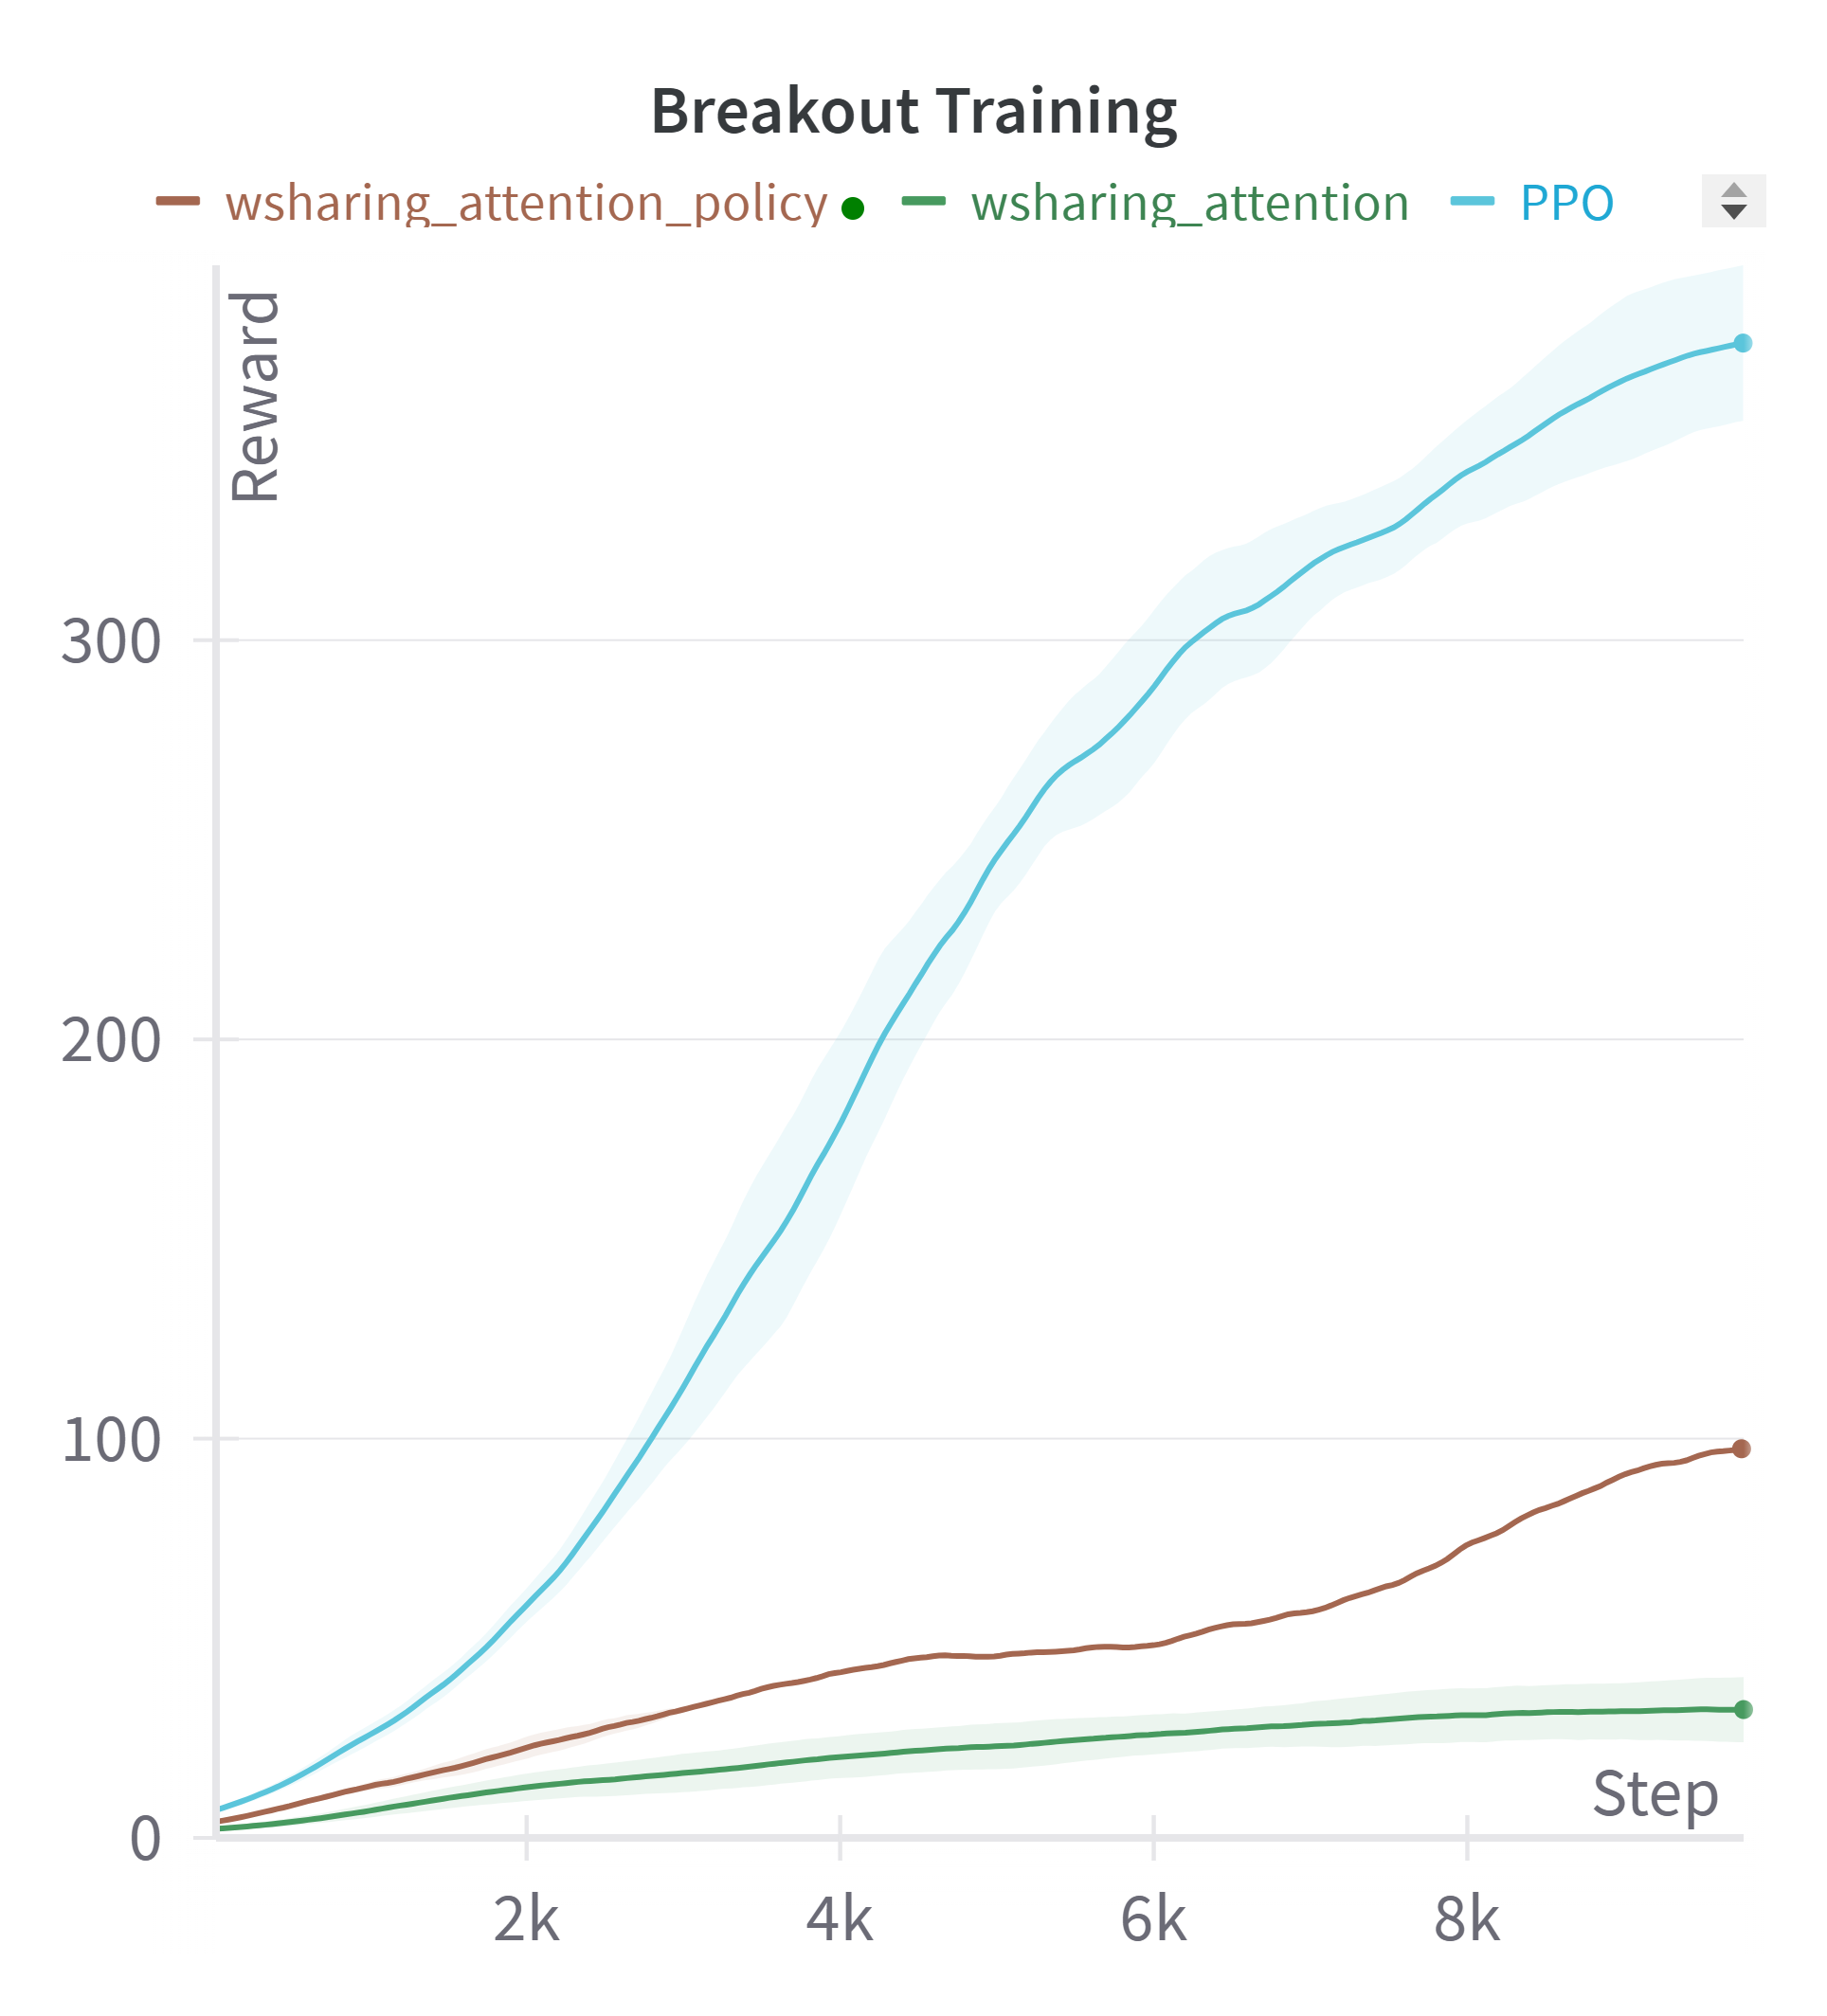
\includegraphics[width=\textwidth]{images/breakout_policy.png}
        \caption{Increasing MLP size}
        \label{fig:breakout_policy}
    \end{subfigure}
    \hfill
    \begin{subfigure}[b]{0.32\textwidth}
        \centering
        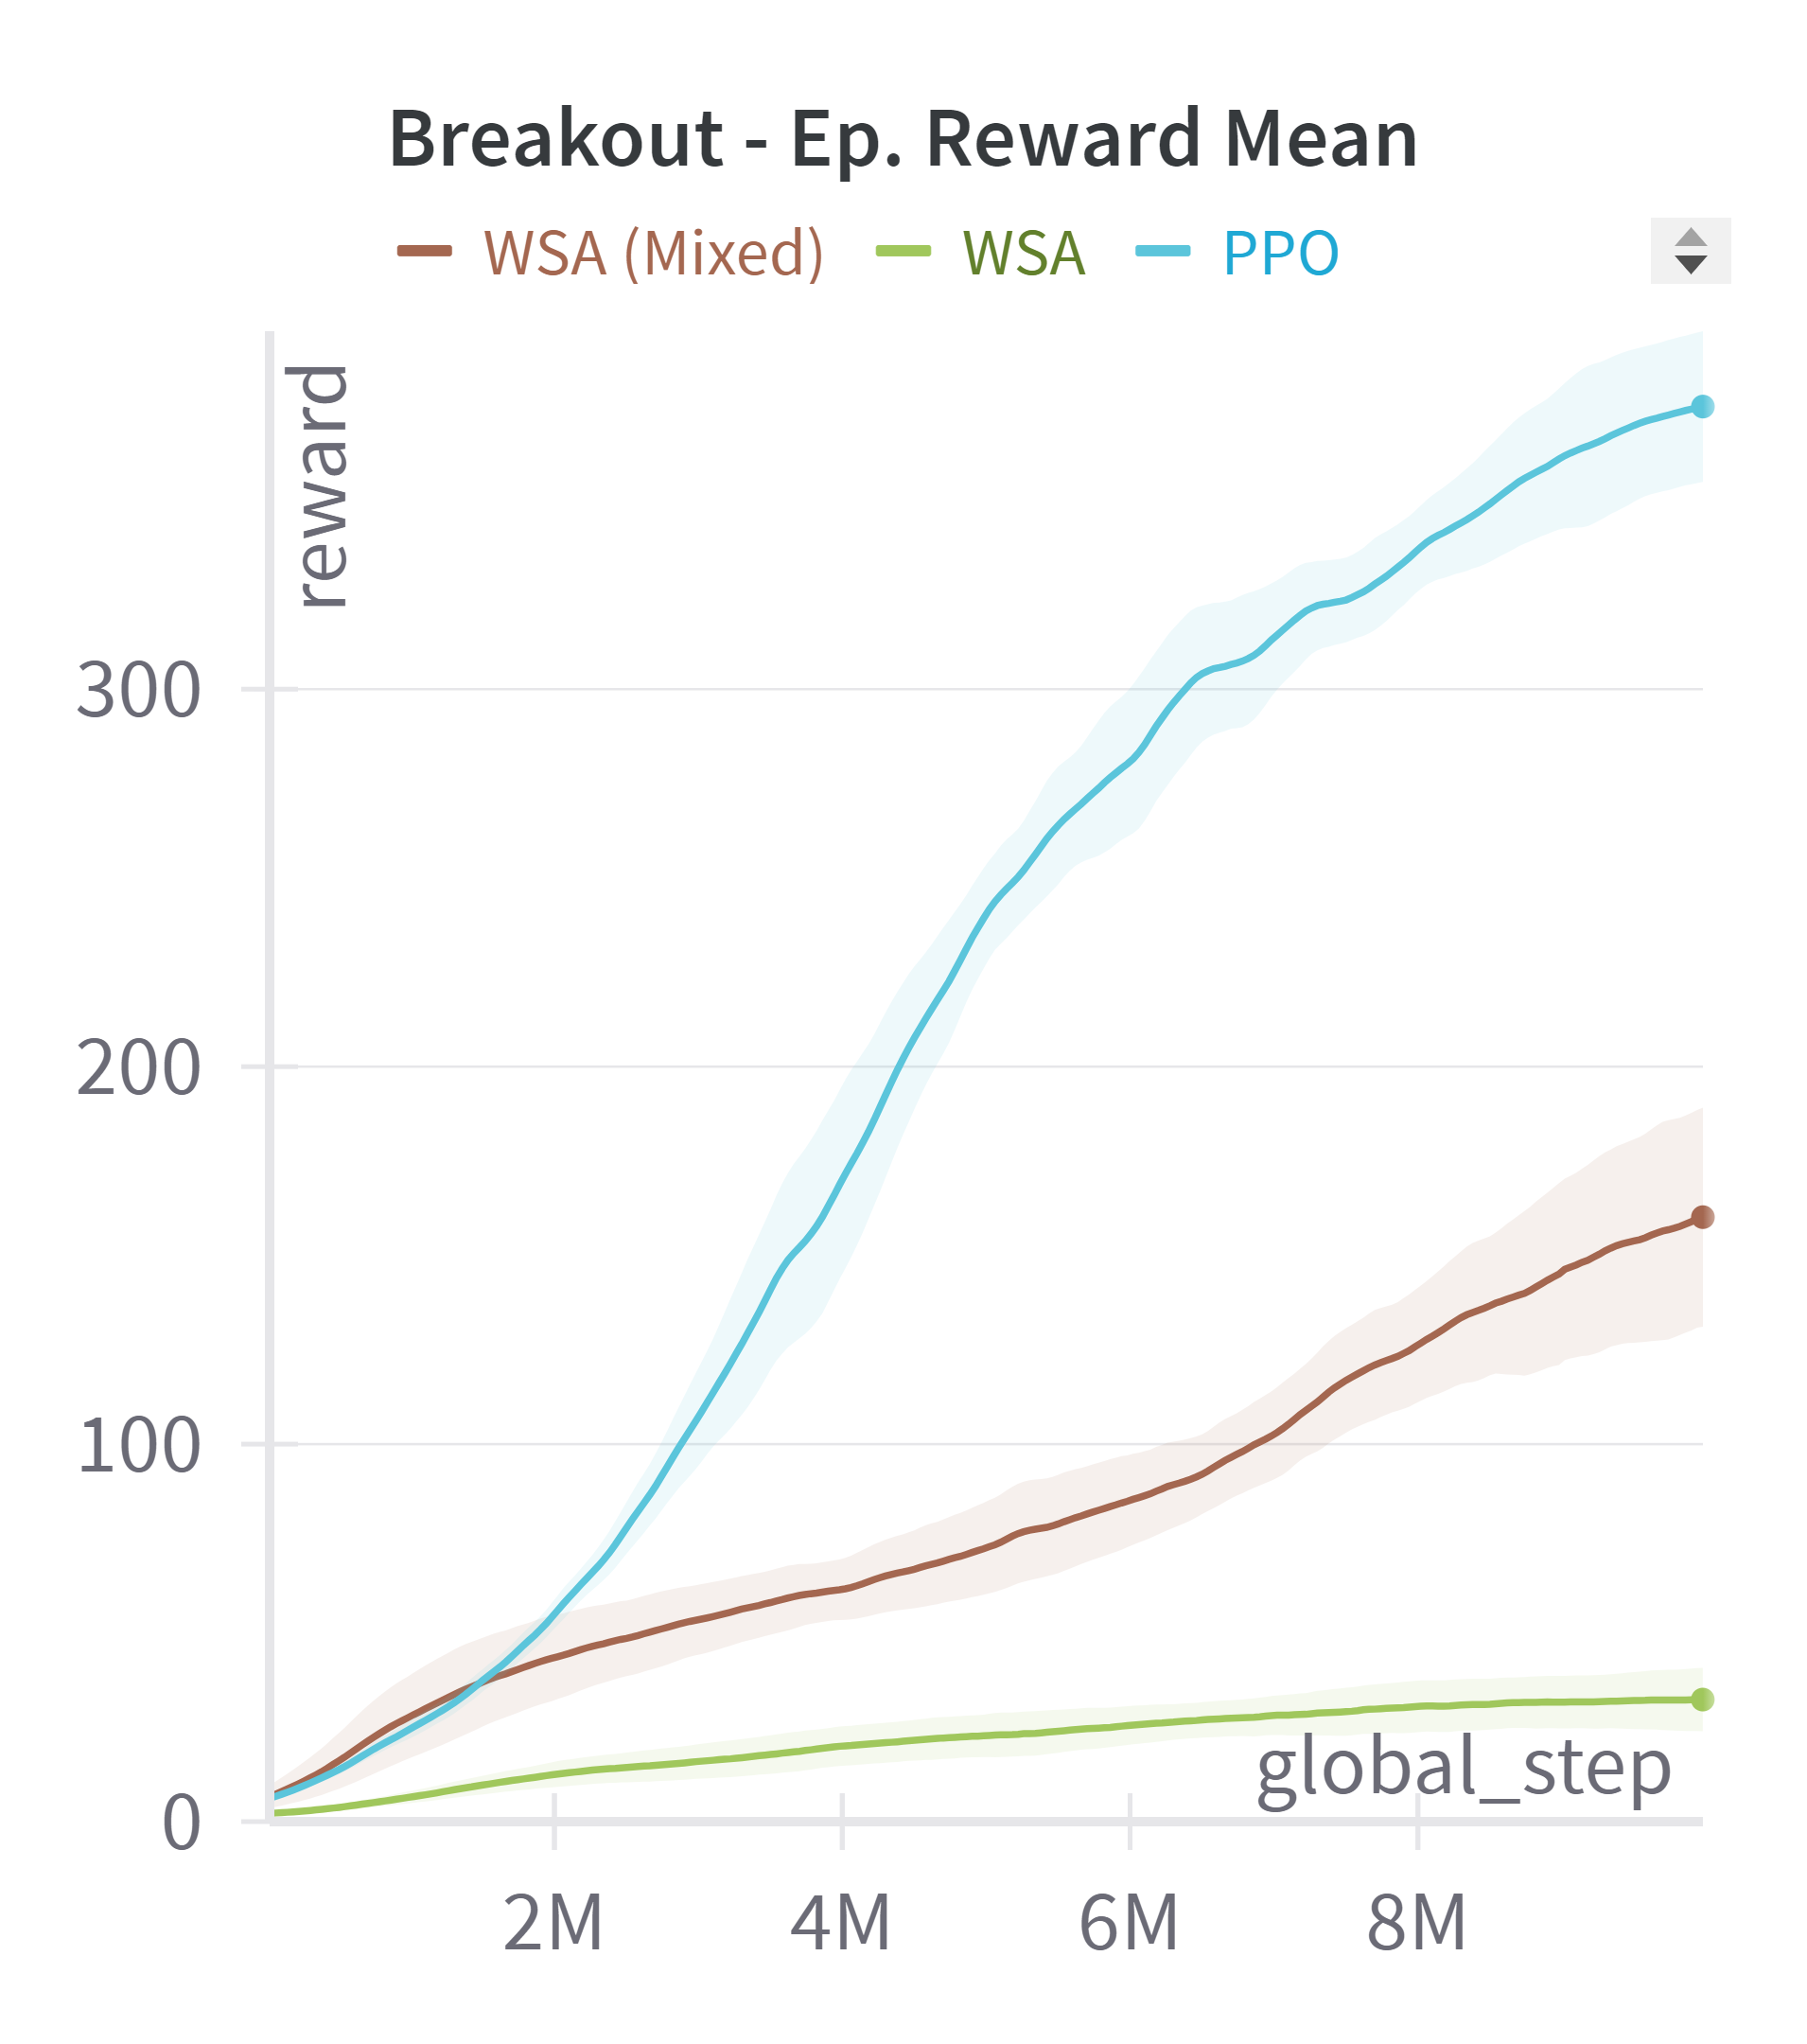
\includegraphics[width=\textwidth]{images/breakout_expert.png}
        \caption{Using Mixed Data}
        \label{fig:breakout_expert}
    \end{subfigure}
    \hfill
    \begin{subfigure}[b]{0.32\textwidth}
        \centering
        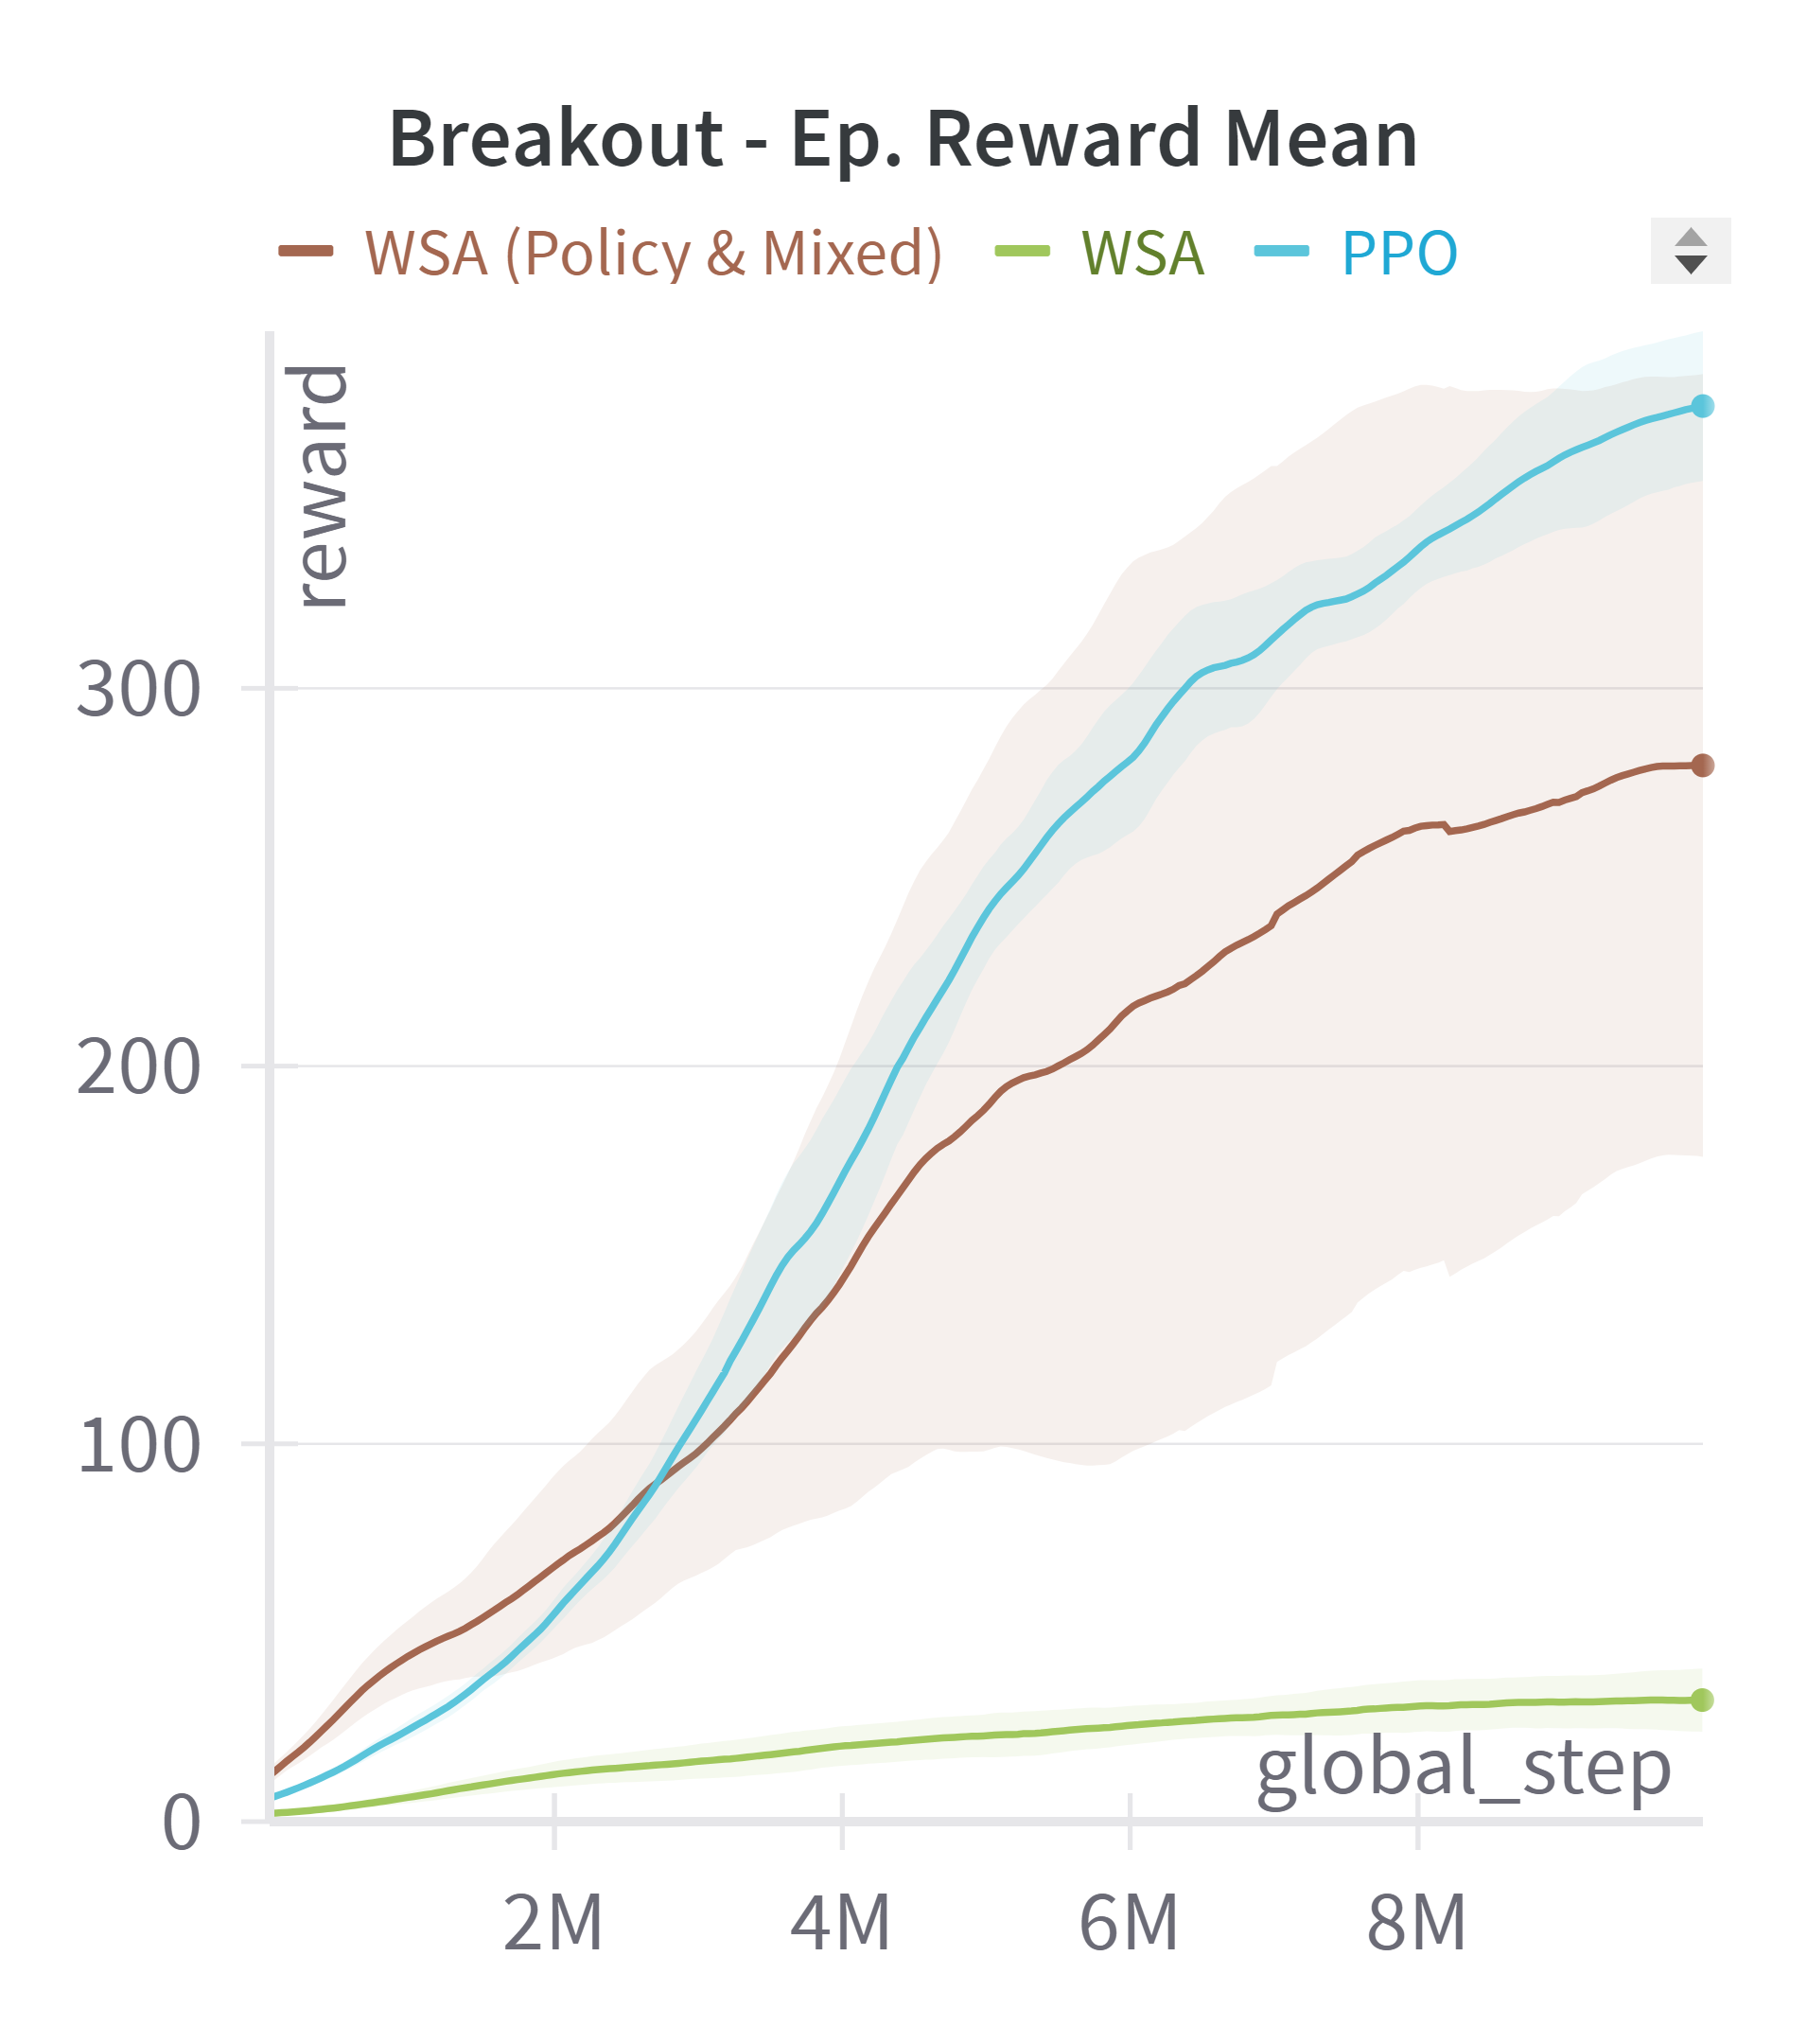
\includegraphics[width=\textwidth]{images/breakout_policy_mixed.png}
        \caption{Mixed Data + Increased MLP}
        \label{fig:breakout_expert_policy}
    \end{subfigure}
    \caption{Performance comparison of WSA with PPO across various strategies on \texttt{Breakout}. Each subfigure displays the average score with the standard deviation shaded. They report the different experiments to improve the performance of WSA: (\ref{fig:breakout_policy}) increasing the size of the \texttt{Fully-Connected Network} on performance, (\ref{fig:breakout_expert}) pre-training the models using random data and expert data, and (\ref{fig:breakout_expert_policy}) combining the effect of increased \texttt{Fully-Connected Network} and expert data during pre-training.}
    \label{fig:breakout_study}
\end{figure}

Before moving on to the next set of experiments, which close the gap between PPO and WSA, we address a key challenge when using pre-trained models in RL. Unlike \texttt{Pong} and \texttt{Ms.Pacman}, where the game screen remains relatively stable, \texttt{Breakout} dynamically evolves as more blocks are removed with score progression. This poses a \textbf{distributional shift} problem between training and test data. Our initial training data, collected from random agents, lacks late game scenarios with few blocks remaining, leading to limitations in FMs performance during evaluation. To tackle the problem and show the consequences of a limited training dataset, we gather new datasets from both random and expert agents to encompass early and late game scenarios.

We retrain all the FMs and RL agents - using a single layer \texttt{Fully-Connected Network}. Significant improvements are observed, as shown in Figure \ref{fig:breakout_expert} and Table \ref{tab:results}, using (\texttt{M}). Notably, WSA demonstrates a substantial increase in the agent's final score (\texttt{156 $\rightarrow$ 345}), approaching PPO performance, and echoing the trends analyzed in Section \ref{sec:results_1} for the other two games. To complete the set of experiments, we also test the combination of the previous configuration. Increased \texttt{Fully-Connected Network} and Mixed datasets (Figure \ref{fig:breakout_expert_policy}, \texttt{PM}) yields the best performing configuration of WSA with slightly lower but competitive score to PPO (\texttt{387 vs 413}). Additionally, Appendix \ref{sec:app-add-exp} reports the same analysis for the other combination modules presented in Figure \ref{fig:breakouttrain}.

Lastly, Figure \ref{fig:inter} illustrates the enhanced \texttt{explainability} provided by WSA. By examining the current frames and the corresponding weights allocated by the shared component to each pre-trained model, one can appreciate agents' decision-making process. The visualization reveals how various FMs are leveraged in distinct contexts, shedding light on agents' dynamic adaptation of its prior knowledge.

\begin{table}[ht]
\begin{minipage}[b]{0.49\linewidth}
\centering
    \begin{tabular}[b]{lll}
                \multicolumn{1}{l}{Environment}  &\multicolumn{1}{l}{\bf Agent} &\multicolumn{1}{l}{\bf Reward} \\
                \hline \\
                \multirow{5}{*}{\texttt{Pong}} & \textbf{CNN} & \textbf{21 $\pm$ 0.00} \\
                                      & RES & 20.85 $\pm$ 0.29 \\
                                      & \textbf{WSA} & \textbf{21 $\pm$ 0.00} \\
                                      & \textbf{PPO} & \textbf{21 $\pm$ 0.00}\\

                                      \hline \\
                \multirow{5}{*}{\texttt{Ms.Pacman}} & CNN & 1801.30 $\pm$ 20.95 \\
                                      & RES & 1369.27 $\pm$ 565.23 \\
                                      &\textbf{WSA} & \textbf{2530.20 $\pm$ 23.09} \\
                                      & \underline{PPO} & \underline{2258.40 $\pm$ 1.42}\\
                                      \hline \\

                \multirow{7}{*}{\texttt{Breakout}}
                                      & CNN & 65.98 $\pm$ 1.62 \\
                                      & FIX & 87.17 $\pm$ 6.87 \\
                                      & WSA & 99.58 $\pm$ 6.66 \\
                                      & WSA (P) & 156.17 $\pm$ 3.59 \\
                                      & WSA (M) & 345.52 $\pm$ 6.47 \\
                                      & \underline{WSA} (PM)& \underline{387.15 $\pm$ 0.43} \\
                                      & \textbf{PPO} & \textbf{413.51 $\pm$ 1.10}\\
    \end{tabular}
    \caption{Performance during \texttt{evaluation} averaged across 5 different seeds.}
    \label{tab:results}
\end{minipage}\hfill
\begin{minipage}[b]{0.49\linewidth}
\centering
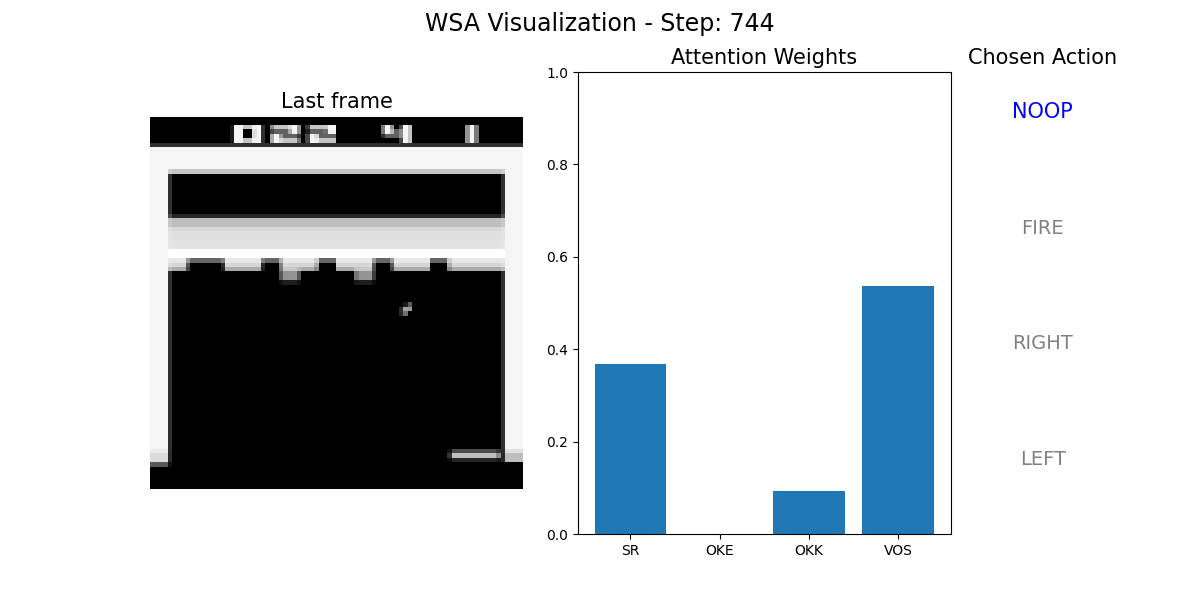
\includegraphics[width=\textwidth]{images/744.png}
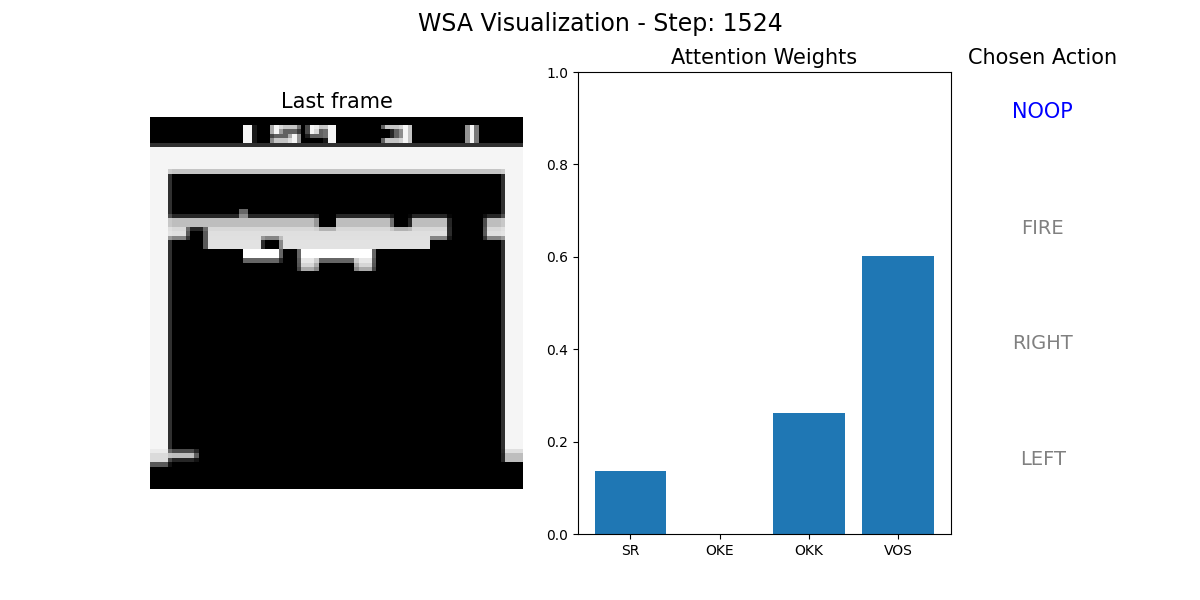
\includegraphics[width=\textwidth]{images/1524.png}
\captionof{figure}{Analyzing WSA explainability across different frames, showcasing the weights assigned to different FMs.}
\label{fig:inter}
\end{minipage}
\end{table}
%%! Author = giaco
%! Date = 16/05/2024

\chapter{Conclusions}
\label{ch:conclusions}
Lorem Ipsum is simply dummy text of the printing and typesetting industry. Lorem Ipsum has been the industry's standard dummy text ever since the 1500s, when an unknown printer took a galley of type and scrambled it to make a type specimen book. It has survived not only five centuries, but also the leap into electronic typesetting, remaining essentially unchanged. It was popularised in the 1960s with the release of Letraset sheets containing Lorem Ipsum passages, and more recently with desktop publishing software like Aldus PageMaker including versions of Lorem Ipsum

%abbiamo notato che i risultati sono meno stabili del più blasonato PPO questo perchè ovviamente c'è bisogno di raffinare l'architettura e i parametri

%Another reason could be the fact that the skills used so far mostly track moving objects, which in Breakout are the ball and the bar. The agent may therefore have little or no information about the bricks, which are a static part of the frame.


%First of all, we have shown that the quality of the training data is crucial for the performance of the agent.
%In particular, in \textit{Breakout} the agent struggled to learn the environment because the training data was not representative of the test data.
%Another limitation of our work is the lack of hyperparameter search.
%We believe that the performance of the agents could be further improved by tuning the hyperparameters, and this is something that we will consider in future work.
%We have shown that our approach is effective with PPO and DQL, but we have not tested other RL algorithms.
%We believe that our approach is general and can be applied to other algorithms, and this is something that we will consider in future work.
%Lastly there are some limitations in the explainability of our approach.
%We have shown that the WSA module can provide insights on how the agent uses the FMs to make decisions, but we have not provided a complete analysis of the explainability of our approach.
%This is something that we will consider in future work.

%In our work, we used pre-trained models provided by the authors of the paper, and we did not perform any hyperparameter search.
%The quality of the pre-trained models can influence the performance of the agent, and a better quality of the pre-trained models can lead to better performance of the agent.


\bibliography{main}

\subsubsection*{Acknowledgments}
\label{sec:ack}
TODO



%%%%%%%%%%%%%%%%%%%%%%%%%%%%%%%%%%%%%%%%%%%%%%%%%%%%%%%%%%%%%%%%
%% Appendices
%%%%%%%%%%%%%%%%%%%%%%%%%%%%%%%%%%%%%%%%%%%%%%%%%%%%%%%%%%%%%%%%
\appendix
%\chapter{Questa è un'appendice}

\lipsum[5]

\section*{Questa è un'altra sezione, ma non viene inserita nell'indice}

\lipsum[6]

\end{document}
